\section{Chassis Assembly}
\label{sec:chassis}

Now that the main PCB of the GRITSBot X is assembled, it needs a chassis to be placed in. This section will detail how to manufacture and assemble the main chassis of the GRITSBOT X. The files associated with the production are available and editable. The Github repository contains Solid Works part files (SLDPRT), Adobe Illustrator files (AI), and PDF files. The PDF files should be able to be used for direct laser cutting of the chassis. The AI files may be used to edit the position of the cuts and duplicate the cuts for more to be produced at once. The SLDPRT files are what may be edited to change the chassis. Feel free to make whatever changes you would like to the design of the robot. This guide will assume that the construction is being done on the files provided.

\subsection{Laser Cutting the Chassis}
\label{sec:laserCut}

The chassis of the GRITSBot X are cut from $1/8$ inch thick and $1/16$ inch thick acrylic. The final cut pieces can be seen in \cref{fig:acrylicChassisCuts}. The files, \texttt{$GRITSBotX\_1\_8.ai$} and \texttt{$GRITSBotX\_1\_16.ai$} are files ready to produce the chassis through a 3D printer. The \texttt{$GRITSBotX\_1\_8$} is meant to create the $1/8$ inch thick acrylic parts and the \texttt{$GRITSBotX\_1\_16$} is meant to create the $1/16$ inch thick acrylic parts. {\color{red}Note}, these are sized for a $36 \times 24$ inch printer and in some cases the document side must be changed. Other alterations may have to be made for the specific laser cutter you are working on to cut and etch the right places in the file.

 %Laser Cut Pieces Picture
\begin{figure}[h!]
\centering
\subfloat[\label{fig:acrylic8}  $1/8$ inch thick acrylic chassis parts.]{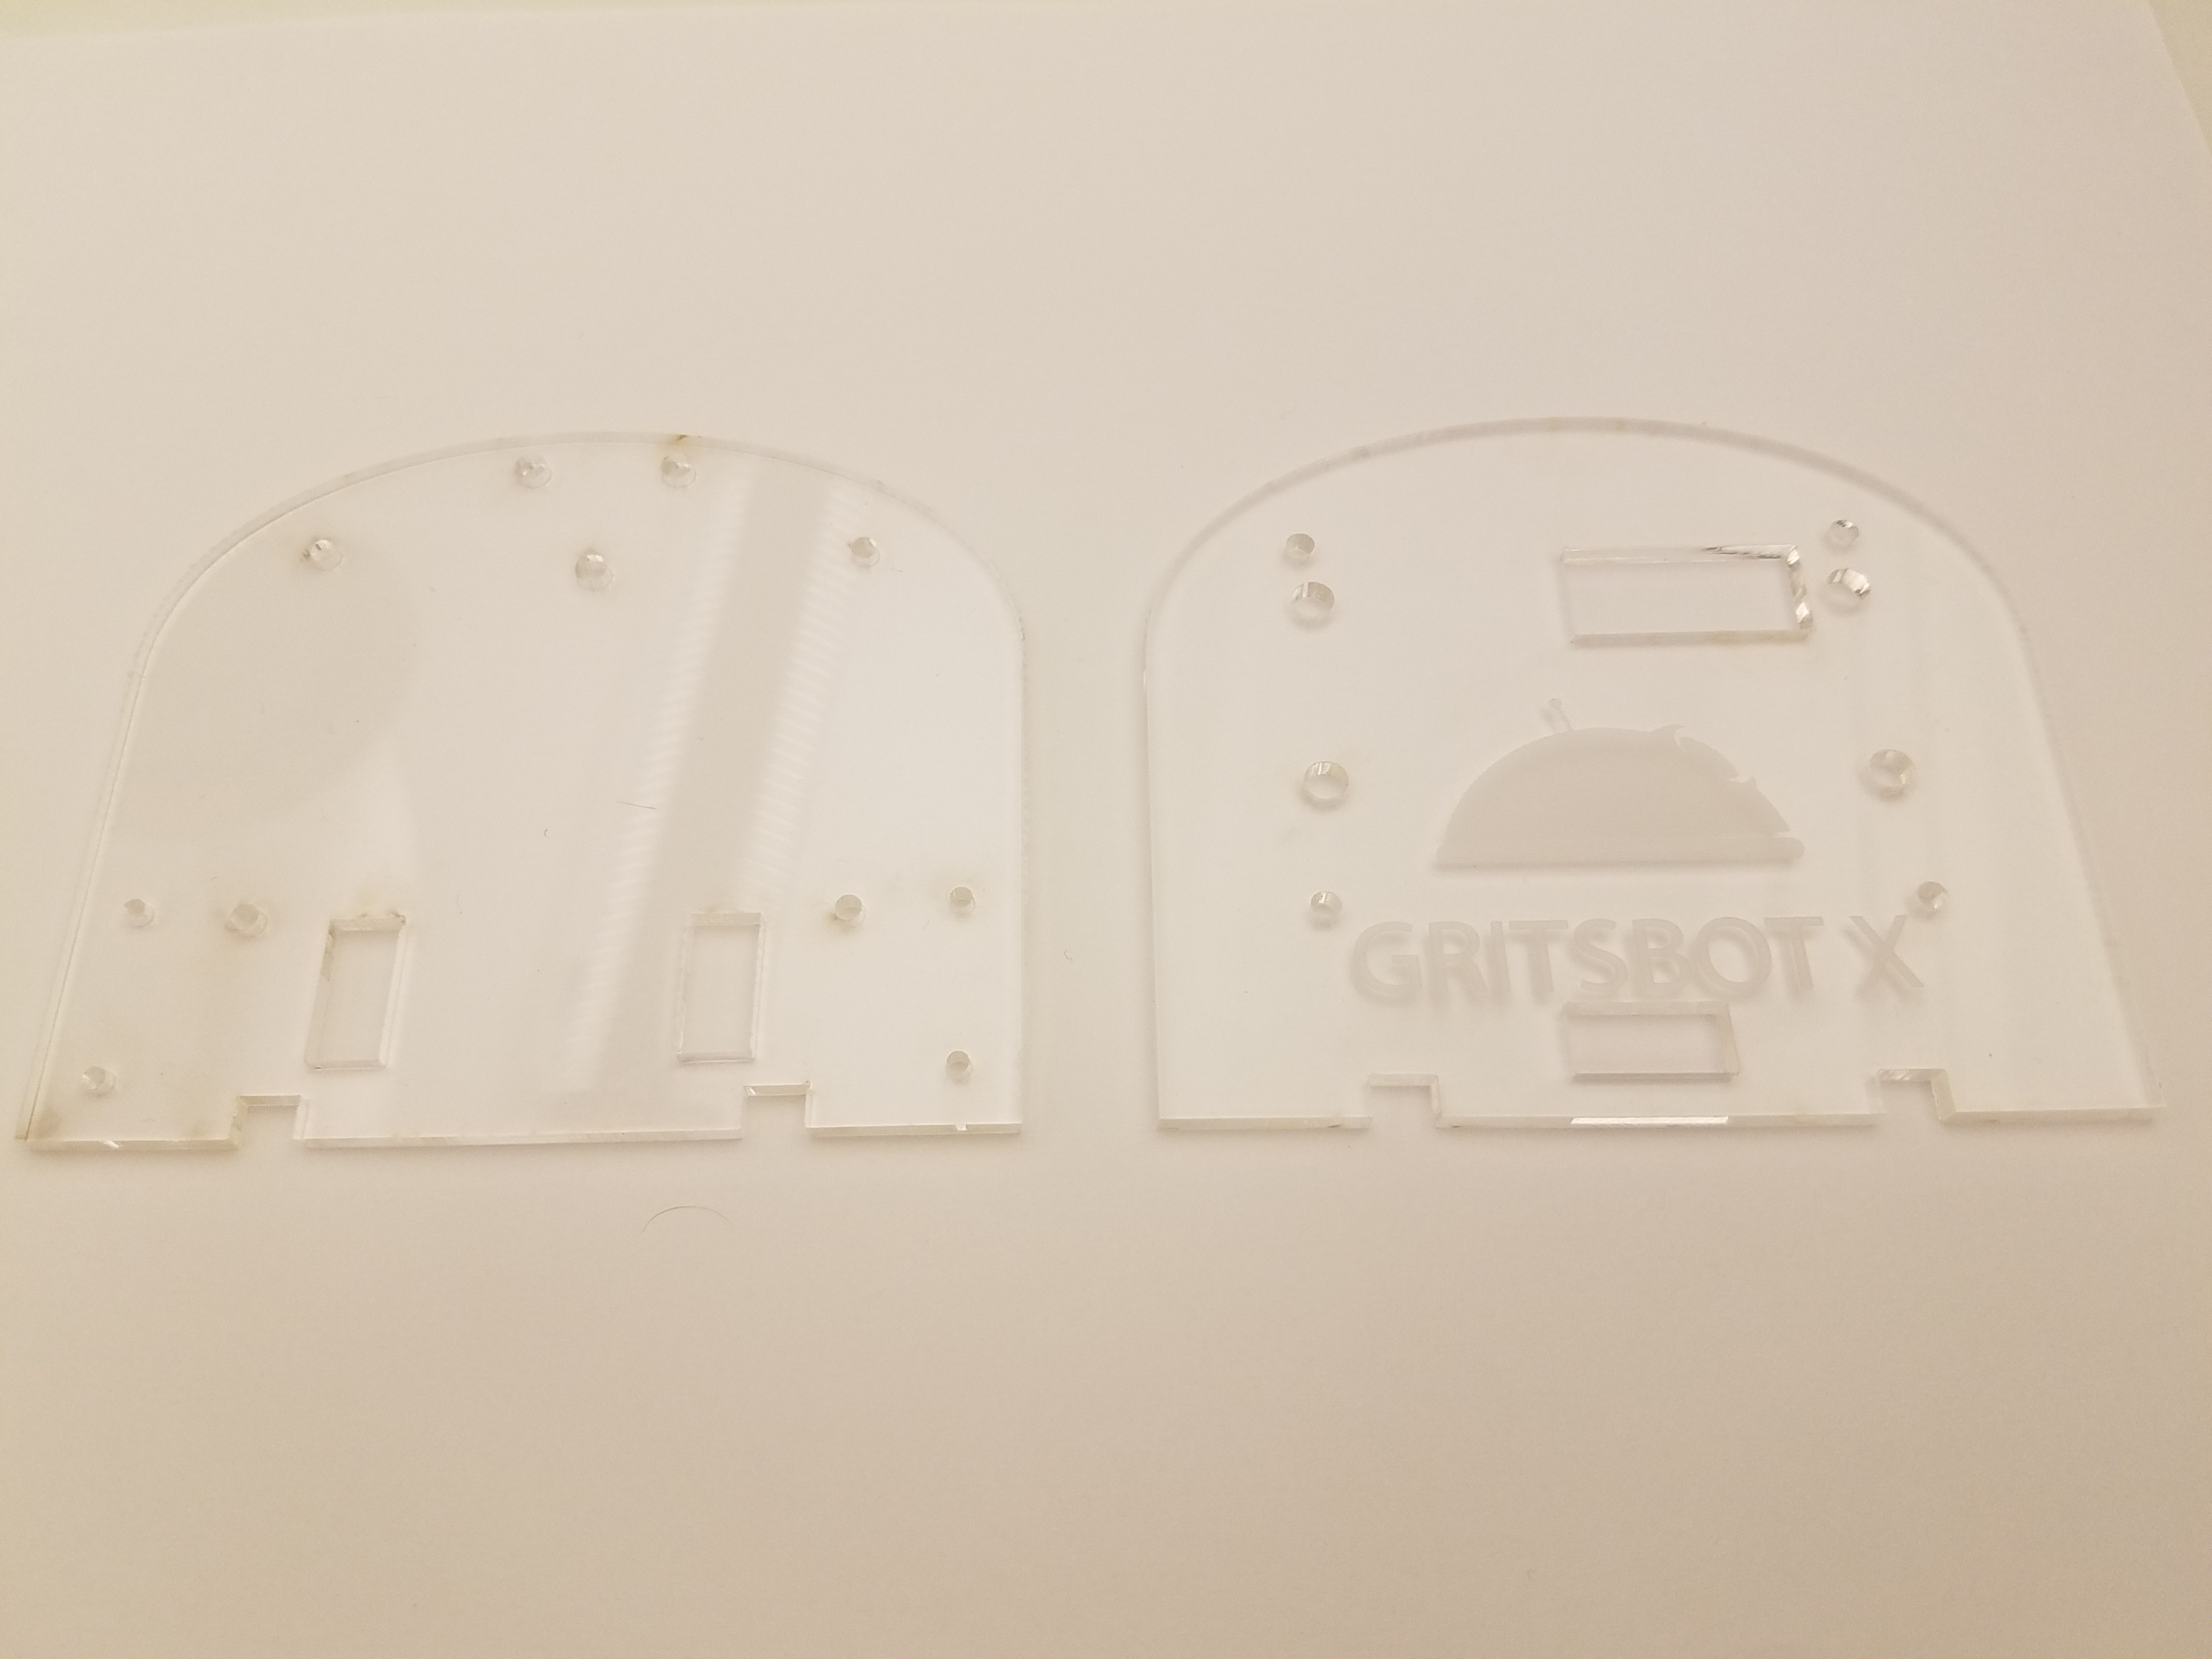
\includegraphics[width=0.45\columnwidth, keepaspectratio]{./figs/20181219_103347.jpg}}
\hfill
\subfloat[\label{fig:acrylic16} $1/16$ inch thick acrylic chassis parts.]{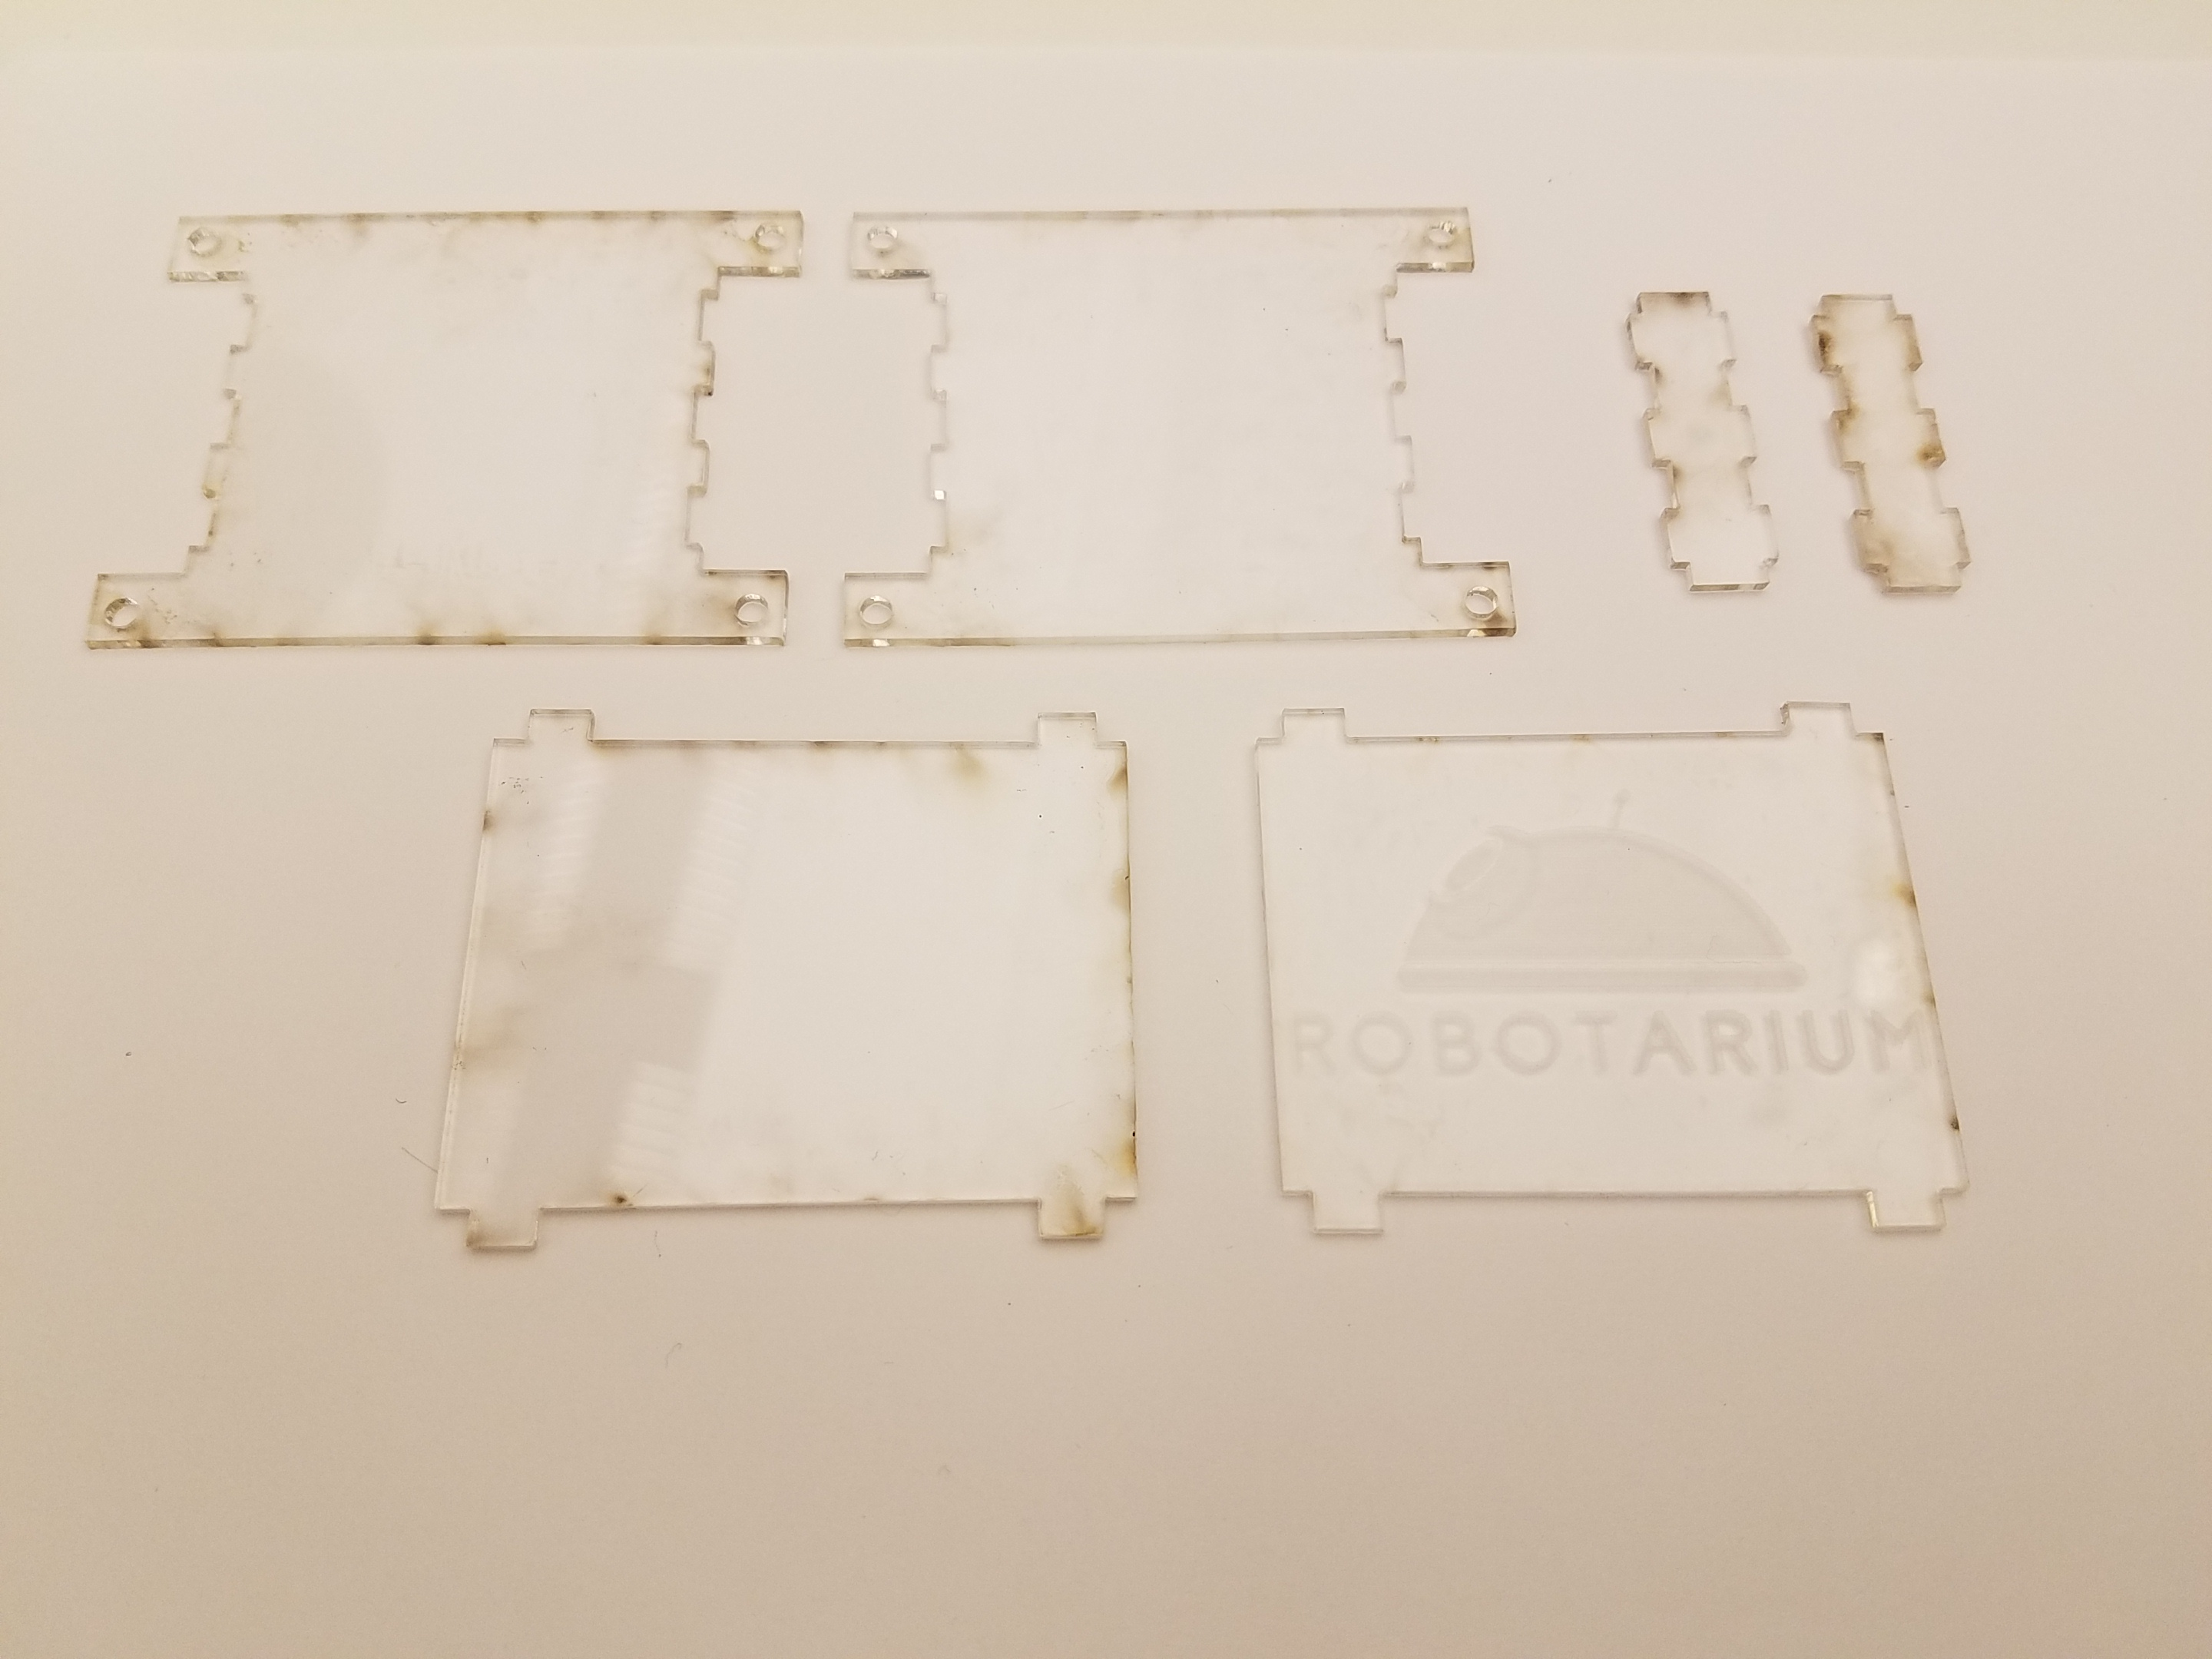
\includegraphics[width=0.45\columnwidth, keepaspectratio]{./figs/20181219_103819.jpg}}\\
\caption{The $1/8$ (a) and $1/16$ (b) inch thick, custom cut acrylic chassis parts for the GRITSBot X.}
\label{fig:acrylicChassisCuts}
\end{figure}
%End Laser Cut Pieces Picture

Now that the acrylic chassis is cut for the GRITSBot X, the final assembly can begin!

\subsection{Assembling the Base}
\label{sec:base}

\subsubsection{Assembly Steps}
\begin{enumerate}
\item Gather the required materials(\cref{sec:baseMaterials}).
\item Assemble the motors and wheels (\cref{sec:motorAssembly}).
\item Put together the Tamiya caster wheel (\cref{sec:casterAssembly}).
\item Attach the motors and caster to the base plate(\cref{sec:baseAssembly}).
\end{enumerate}

\subsubsection{Required Materials}
\label{sec:baseMaterials}

As with the other sections, the first step is to gather the required materials. These are pictured in \cref{fig:baseMaterials} and listed in \cref{tab:baseMaterials}.

  %Begin Base Part Table
 \begin{table}[h!]
 \centering
\begin{tabular}{lc}
\rowcolor[HTML]{C0C0C0} 
\textbf{Part}  & \textbf{Number Required} 		\\
Acrylic Base Plate			&  1	\\
\rowcolor[HTML]{C0C0C0} 
Wheel               				& 2	\\
Micro-Metal Gear Motor	& 2	\\
\rowcolor[HTML]{C0C0C0} 
Motor Bracket Assembly	& 2   \\
Tamiya Caster Assembly	& 1	\\
\rowcolor[HTML]{C0C0C0} 
Compression Spring		& 3   \\
M3-20 Screw				& 3	\\
\rowcolor[HTML]{C0C0C0} 
M3 Locknut				& 3  
\end{tabular}
\caption{The parts required to assemble the base of the GRITSBot X. \label{tab:baseMaterials}}
\end{table}
 %End Base Part Table
 
 %Base Materials Picture
\begin{figure}[h!]
\centering
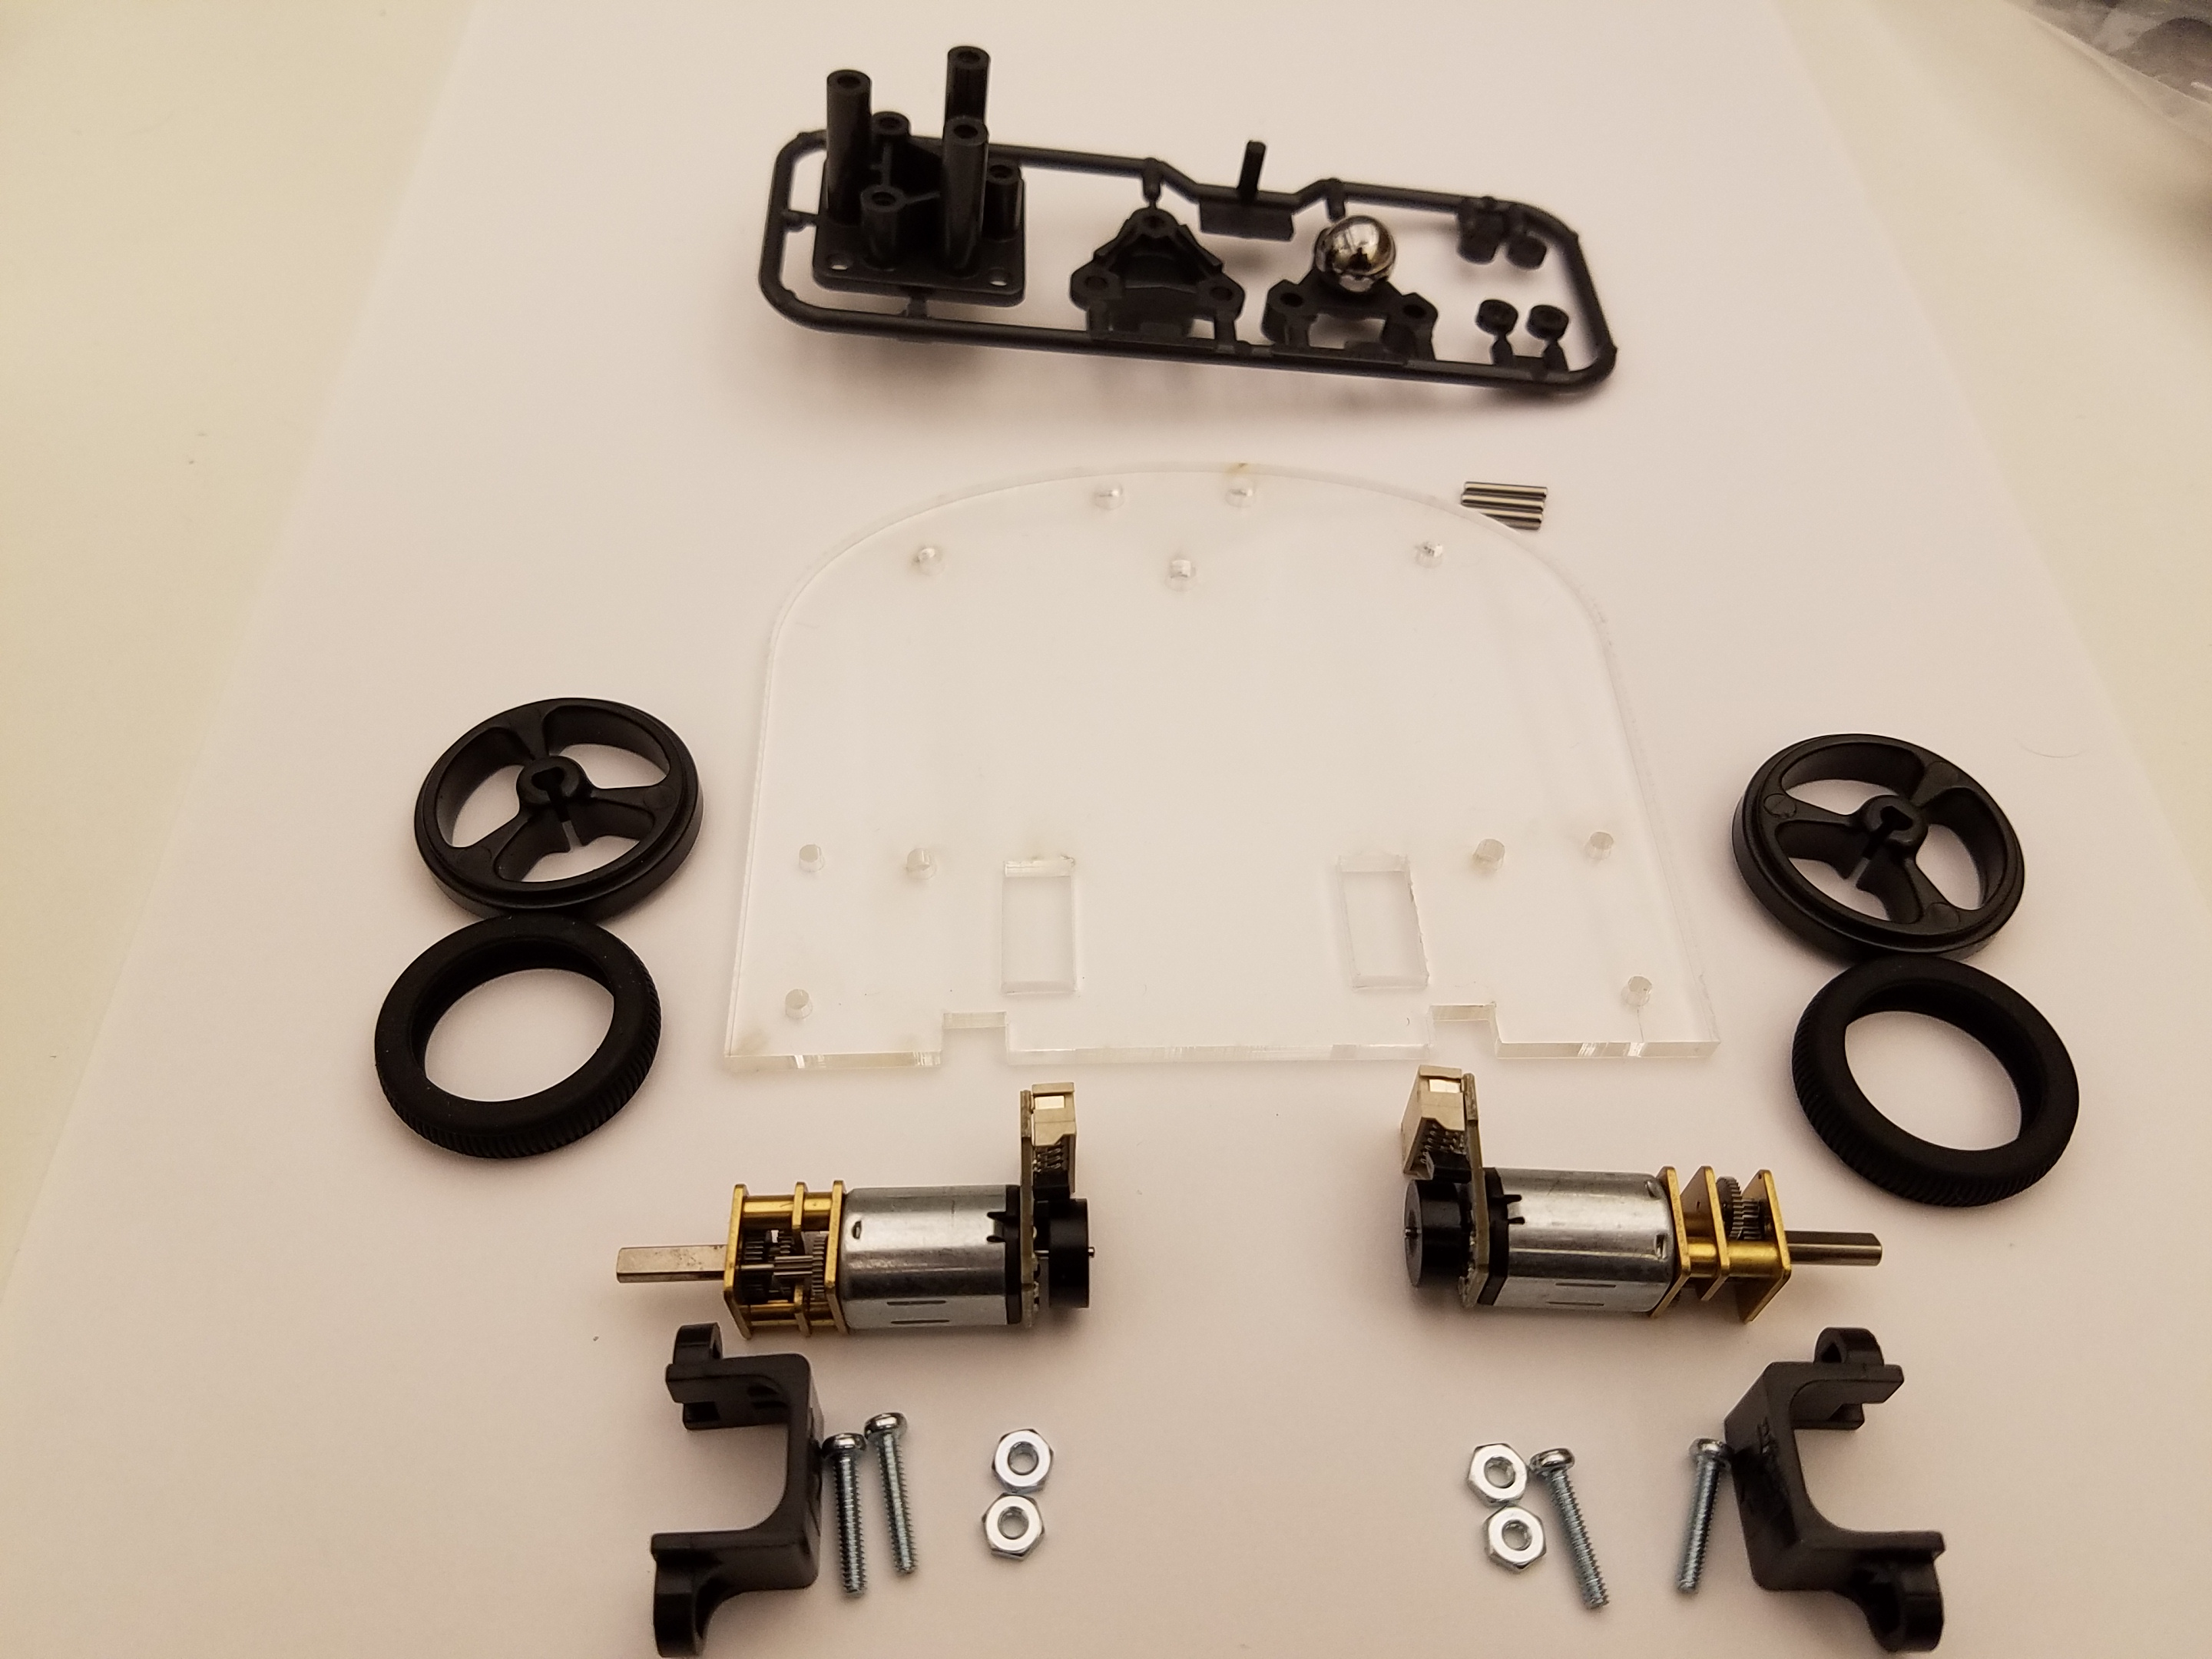
\includegraphics[width=0.65\columnwidth, keepaspectratio]{./figs/20181219_104828.jpg}
\caption{The materials needed to construct the base of the GRITSBot X.}
\label{fig:baseMaterials}
\end{figure}
%End Base Materials Picture

The acrylic base plate should have been laser cut in the previous step. The base plate can be recognized by the three screw holes in a triangular formation in the middle of the curved side of the chassis. This serves as the foundation of the GRITSBot X. The two wheels should come in one package from Pololu with the rubber tires separate from the plastic rims. The micro-metal gear motors from DFRobot come individually with corresponding jumper wires (not pictured here). Do not discard those, they will be used later.  The motor bracket assembly from Pololu should come as a pair with the nuts and screws pictured.  If the screws and nuts are lost they can easily be replaced, they are $\#2-56x7/16''$ screws with $\#2-56$ nuts. The Tamiya caster assembly come in packs of two. You only need one of the two and can keep the other for spare parts or keep this in mind when mass producing. The compression springs are meant as a pseudo suspension on the front caster to alleviate rattling and noise while the M3-20 screw and locknut keep the caster firmly attached to the base.

\subsubsection{Motor and Wheel Assembly}
\label{sec:motorAssembly}

The motor and wheel assembly is fairly straight forward but for consistency between robots details and tips are provided in this section. First, place the tires around the plastic rims. The tires are pretty elastic and can be stretched rather far. The tires on the rims should look like \cref{fig:tires} when finished.

%Tires Picture
\begin{figure}[h!]
\centering
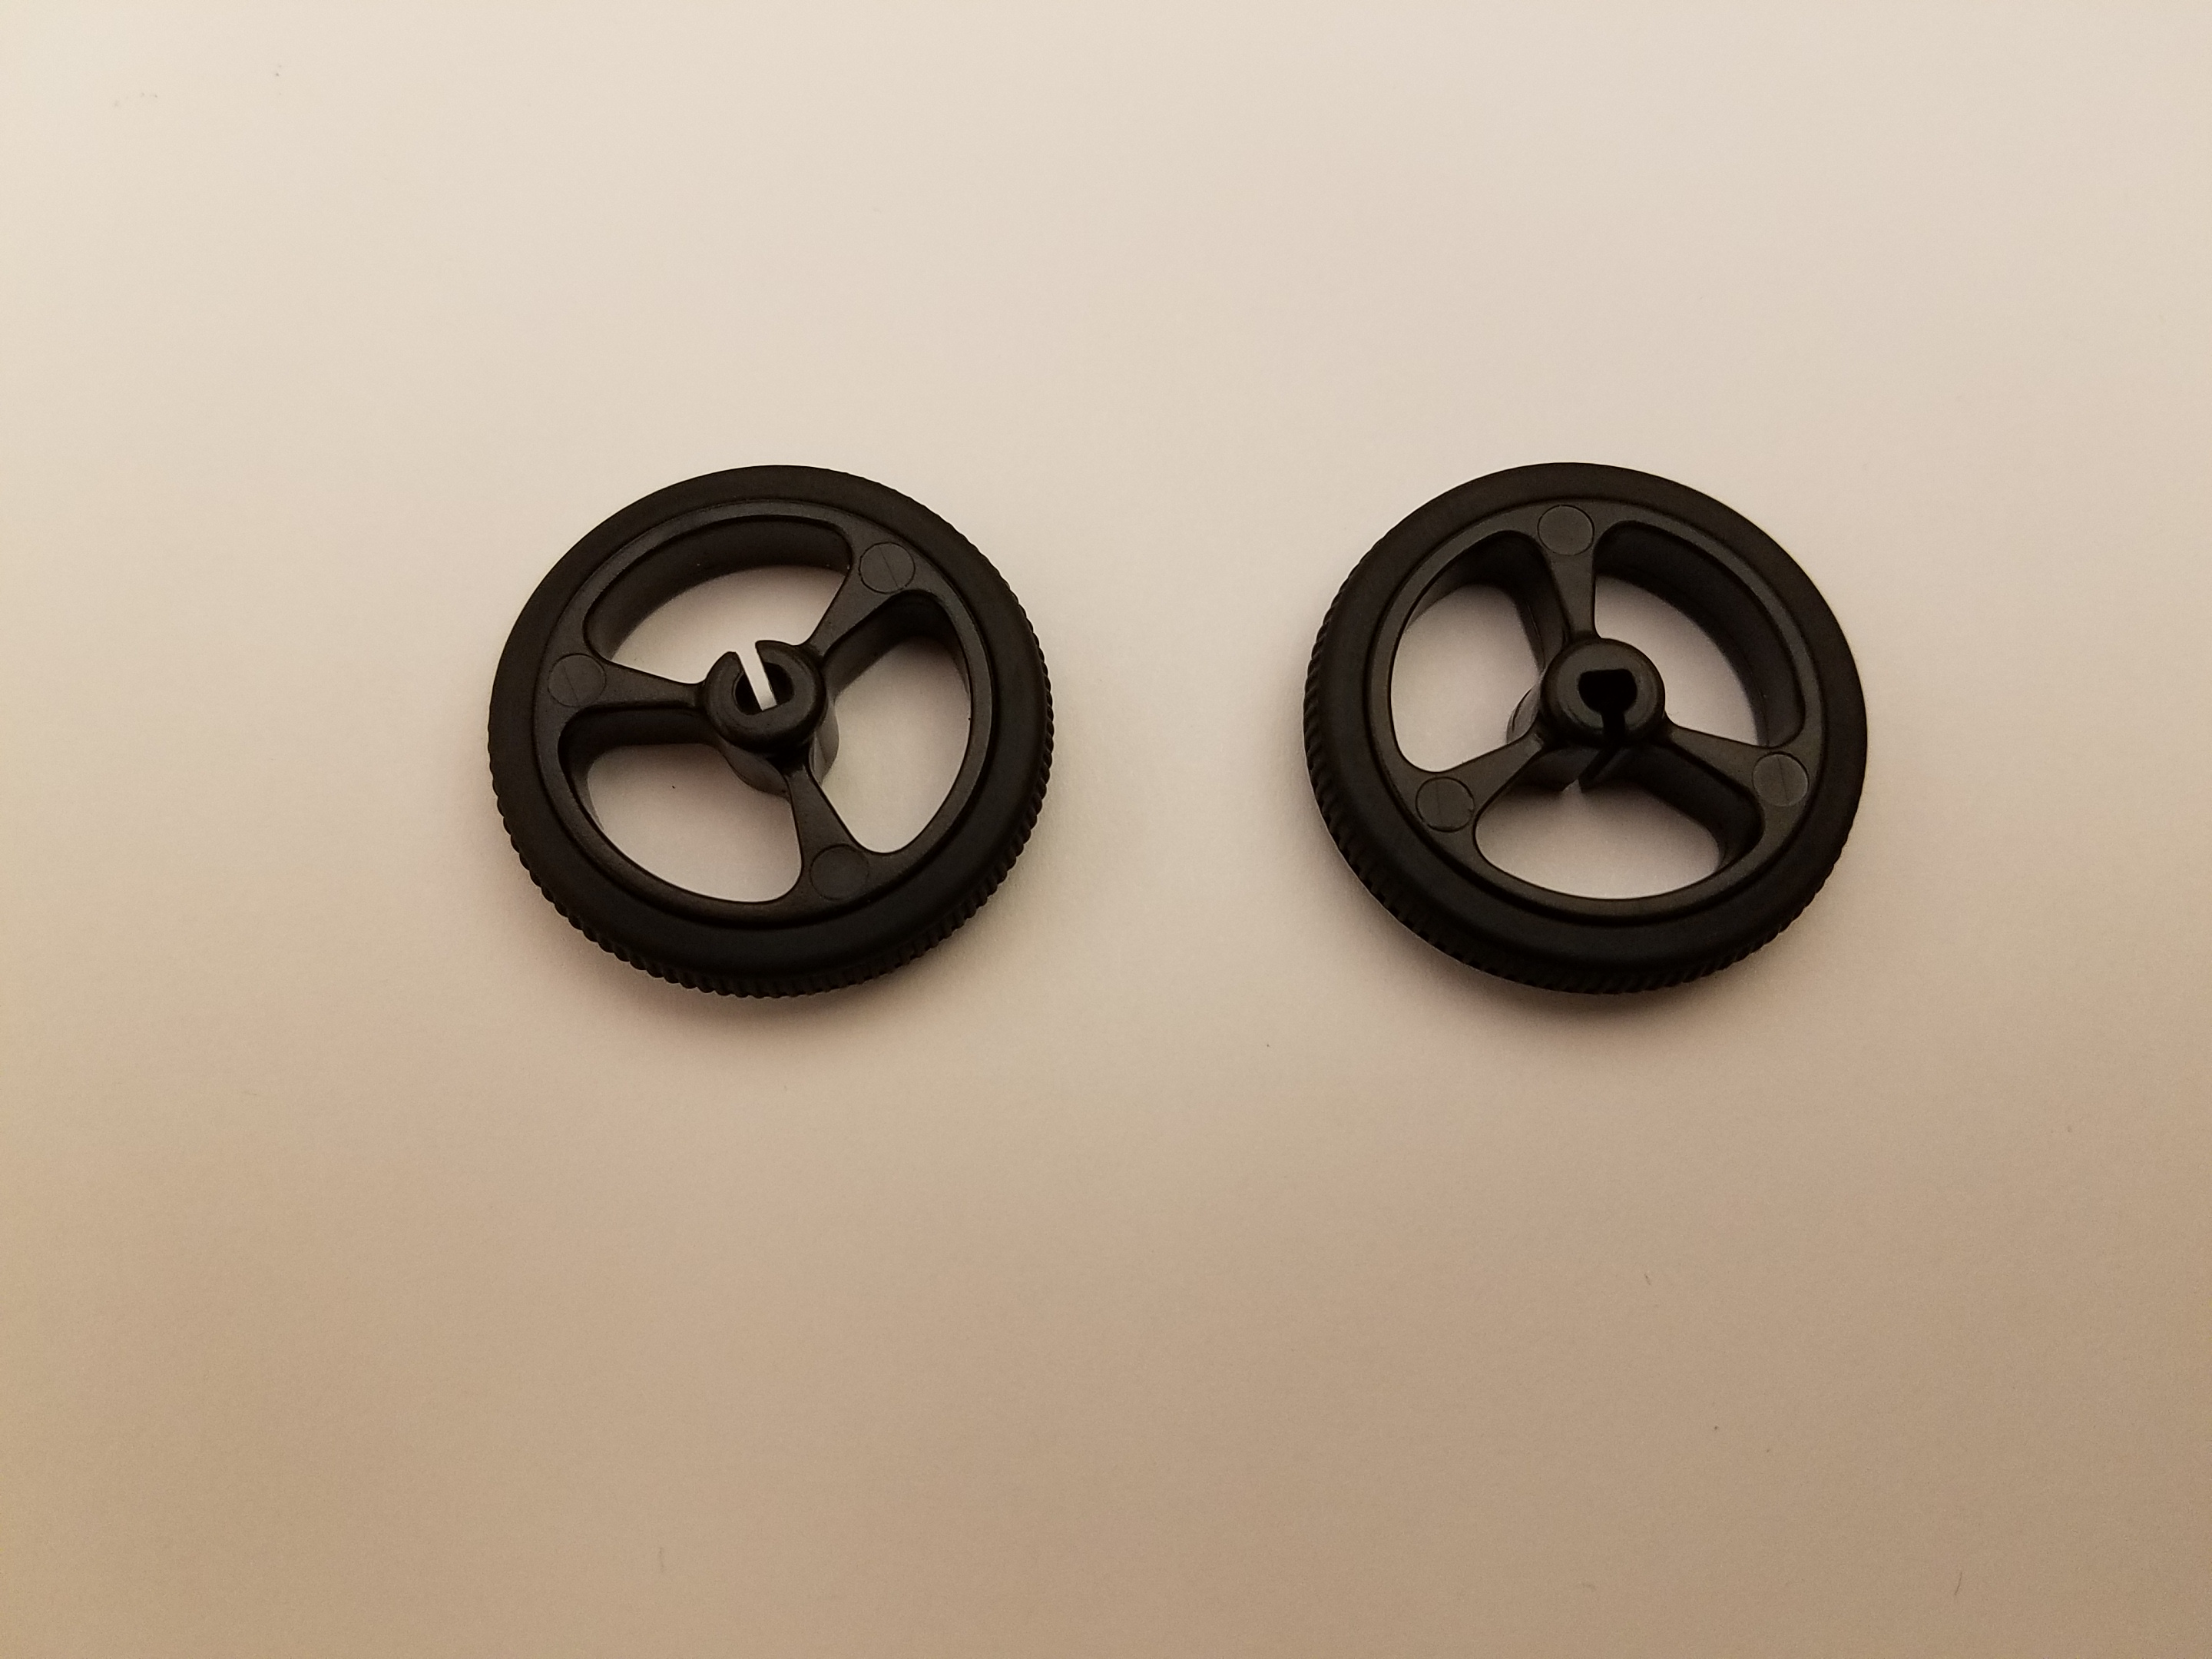
\includegraphics[width=0.65\columnwidth, keepaspectratio]{./figs/20181219_112356.jpg}
\caption{GRITSBot X wheels fully assembled.}
\label{fig:tires}
\end{figure}
%End Tires Picture

These assembled wheels attach to the motors through a D-shaft. It is important to note the wheels have a flat side and side that sticks out. When pressing the wheel onto the D-shaft of the motor, make sure the flat side of the wheel is facing away from the motor. An easy way to attach the wheel to the D-shaft is to press the motor onto a flat surface through the wheel as pictured in \cref{fig:motorAssembly}. If you assemble this way, {\color{red}{be careful}} the encoder PCB is fragile and the magnetic disc can easily be moved. You are most likely to bend or break off the hall effect sensors (black rectangles sticking out of the PCB), so be careful where you place your hands/fingers when doing this.

%Motor Assembly Picture
\begin{figure}[h!]
\centering
\subfloat[\label{fig:pressMotor}  Pressing the motor D-shaft into the wheel.]{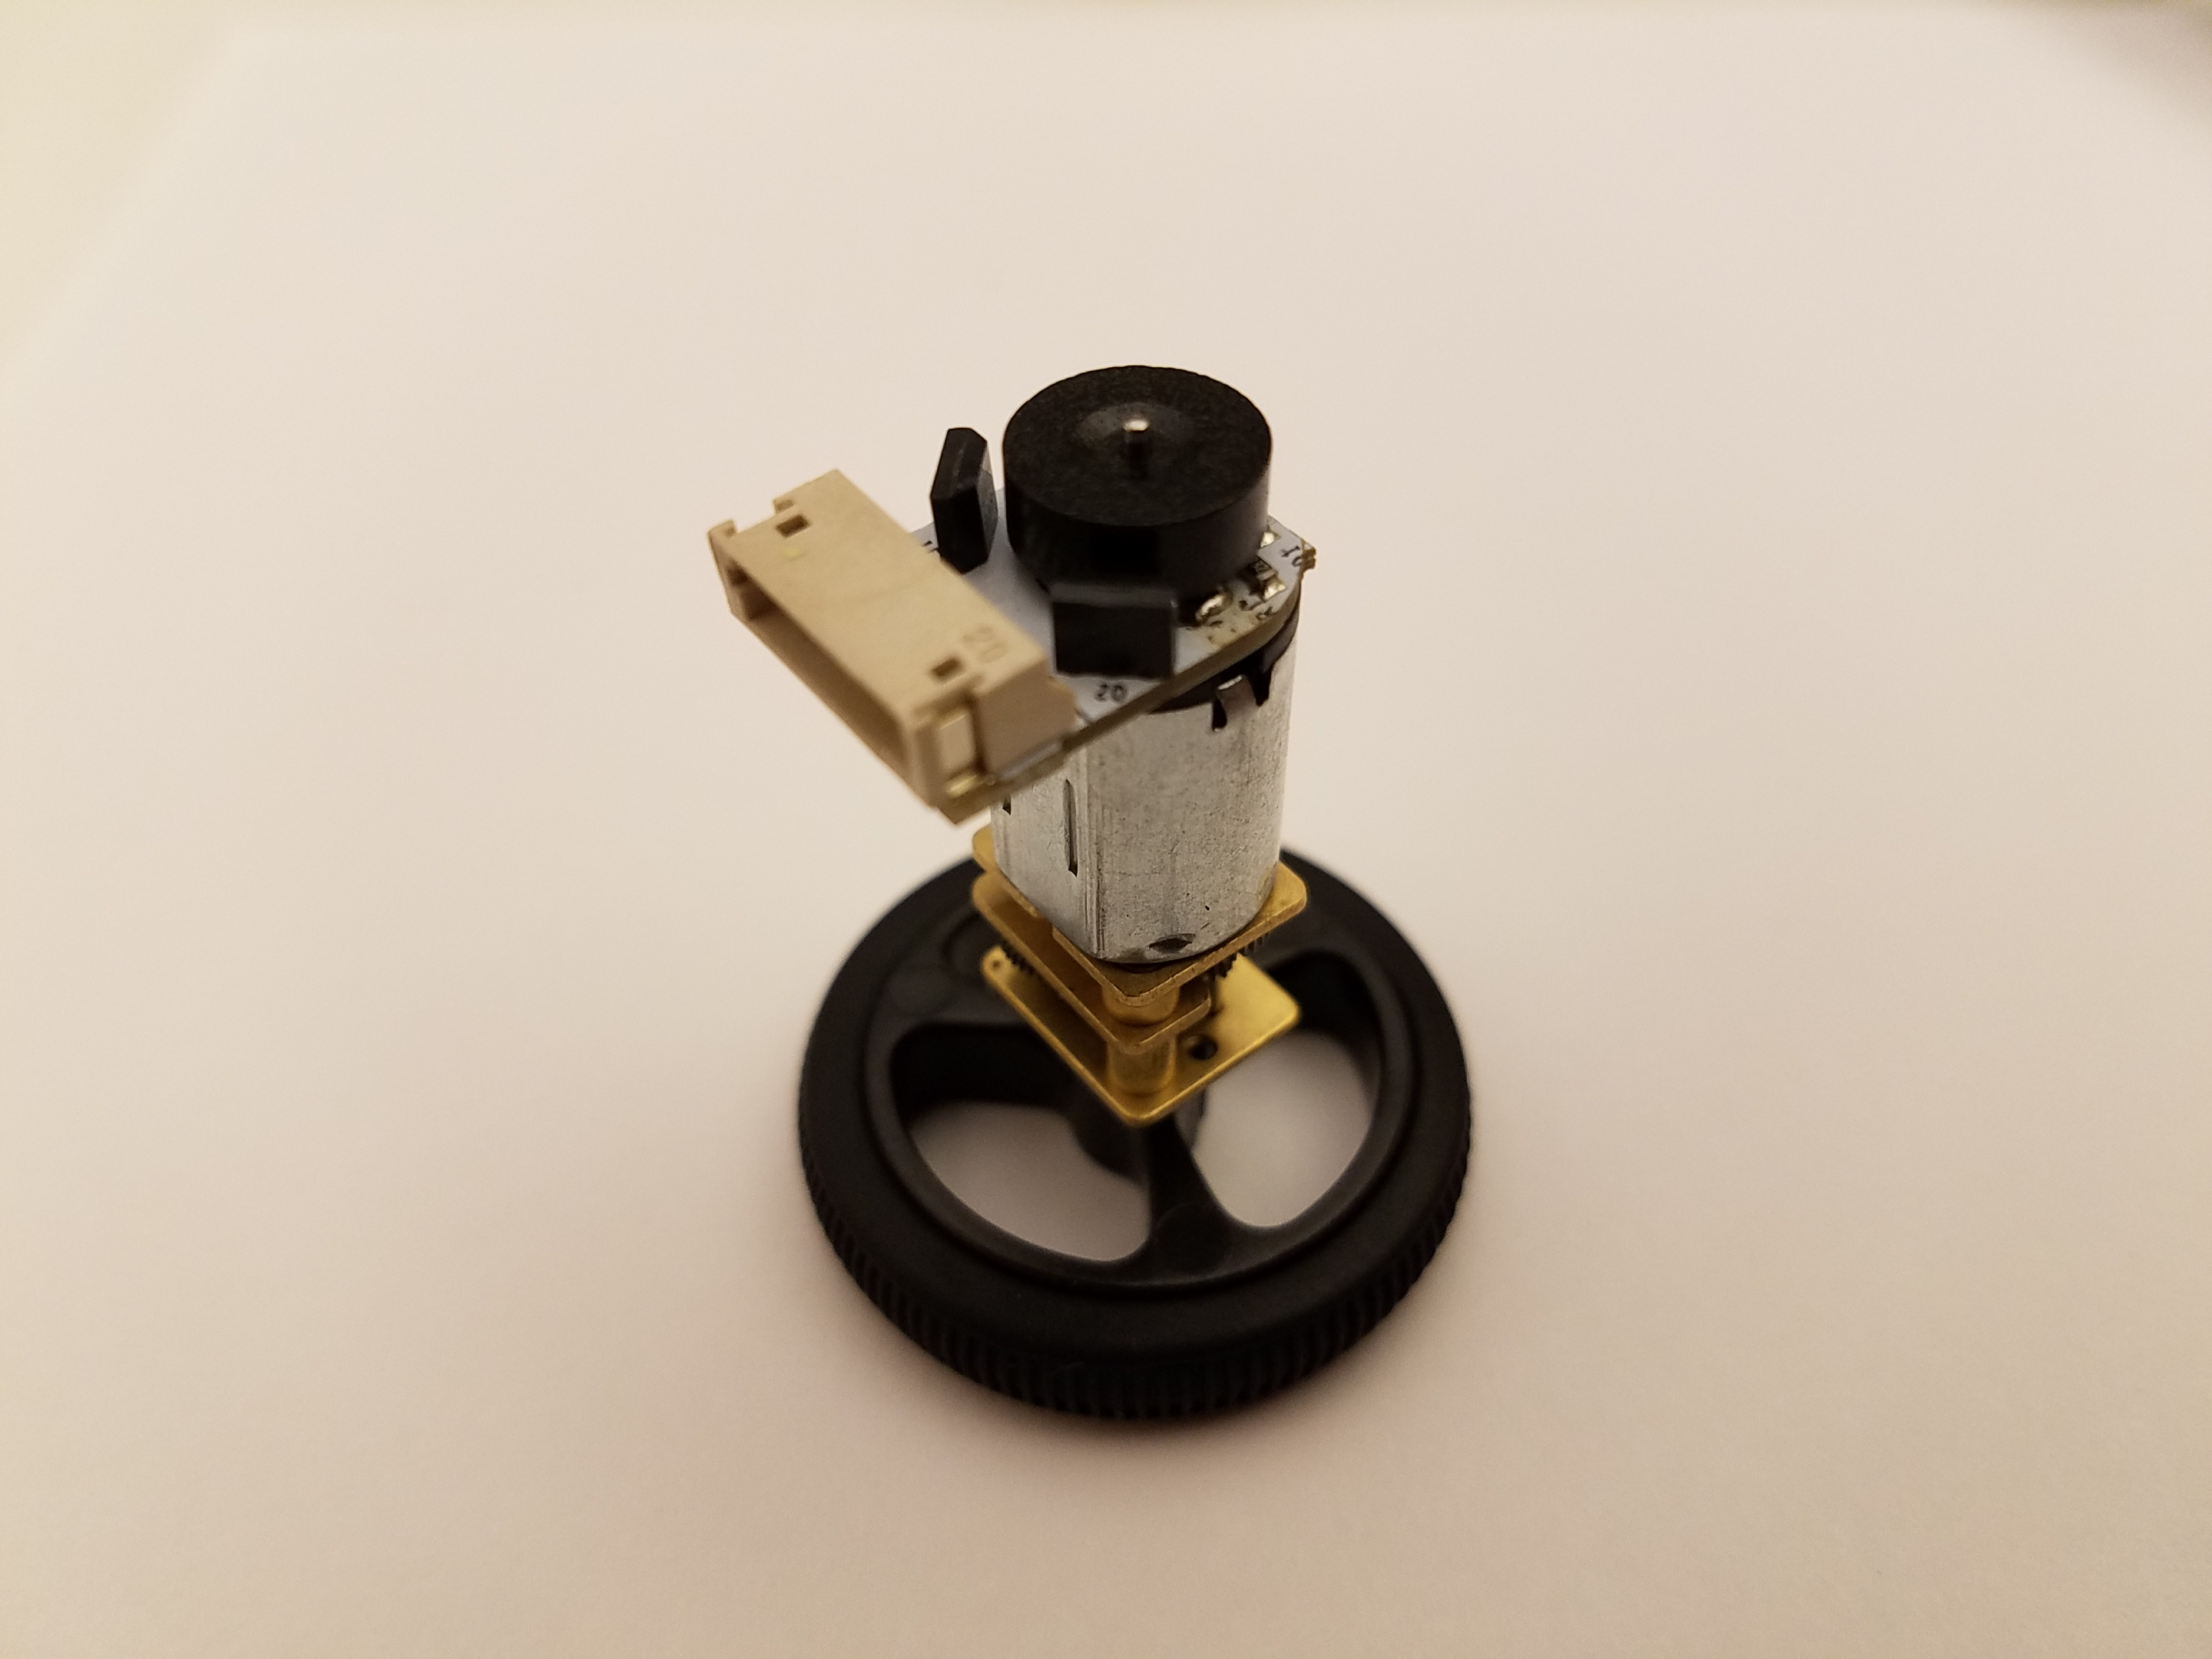
\includegraphics[width=0.45\columnwidth, keepaspectratio]{./figs/20181219_112426.jpg}}
\hfill
\subfloat[\label{fig:motorSide} Side view of the motor and wheel assembly.]{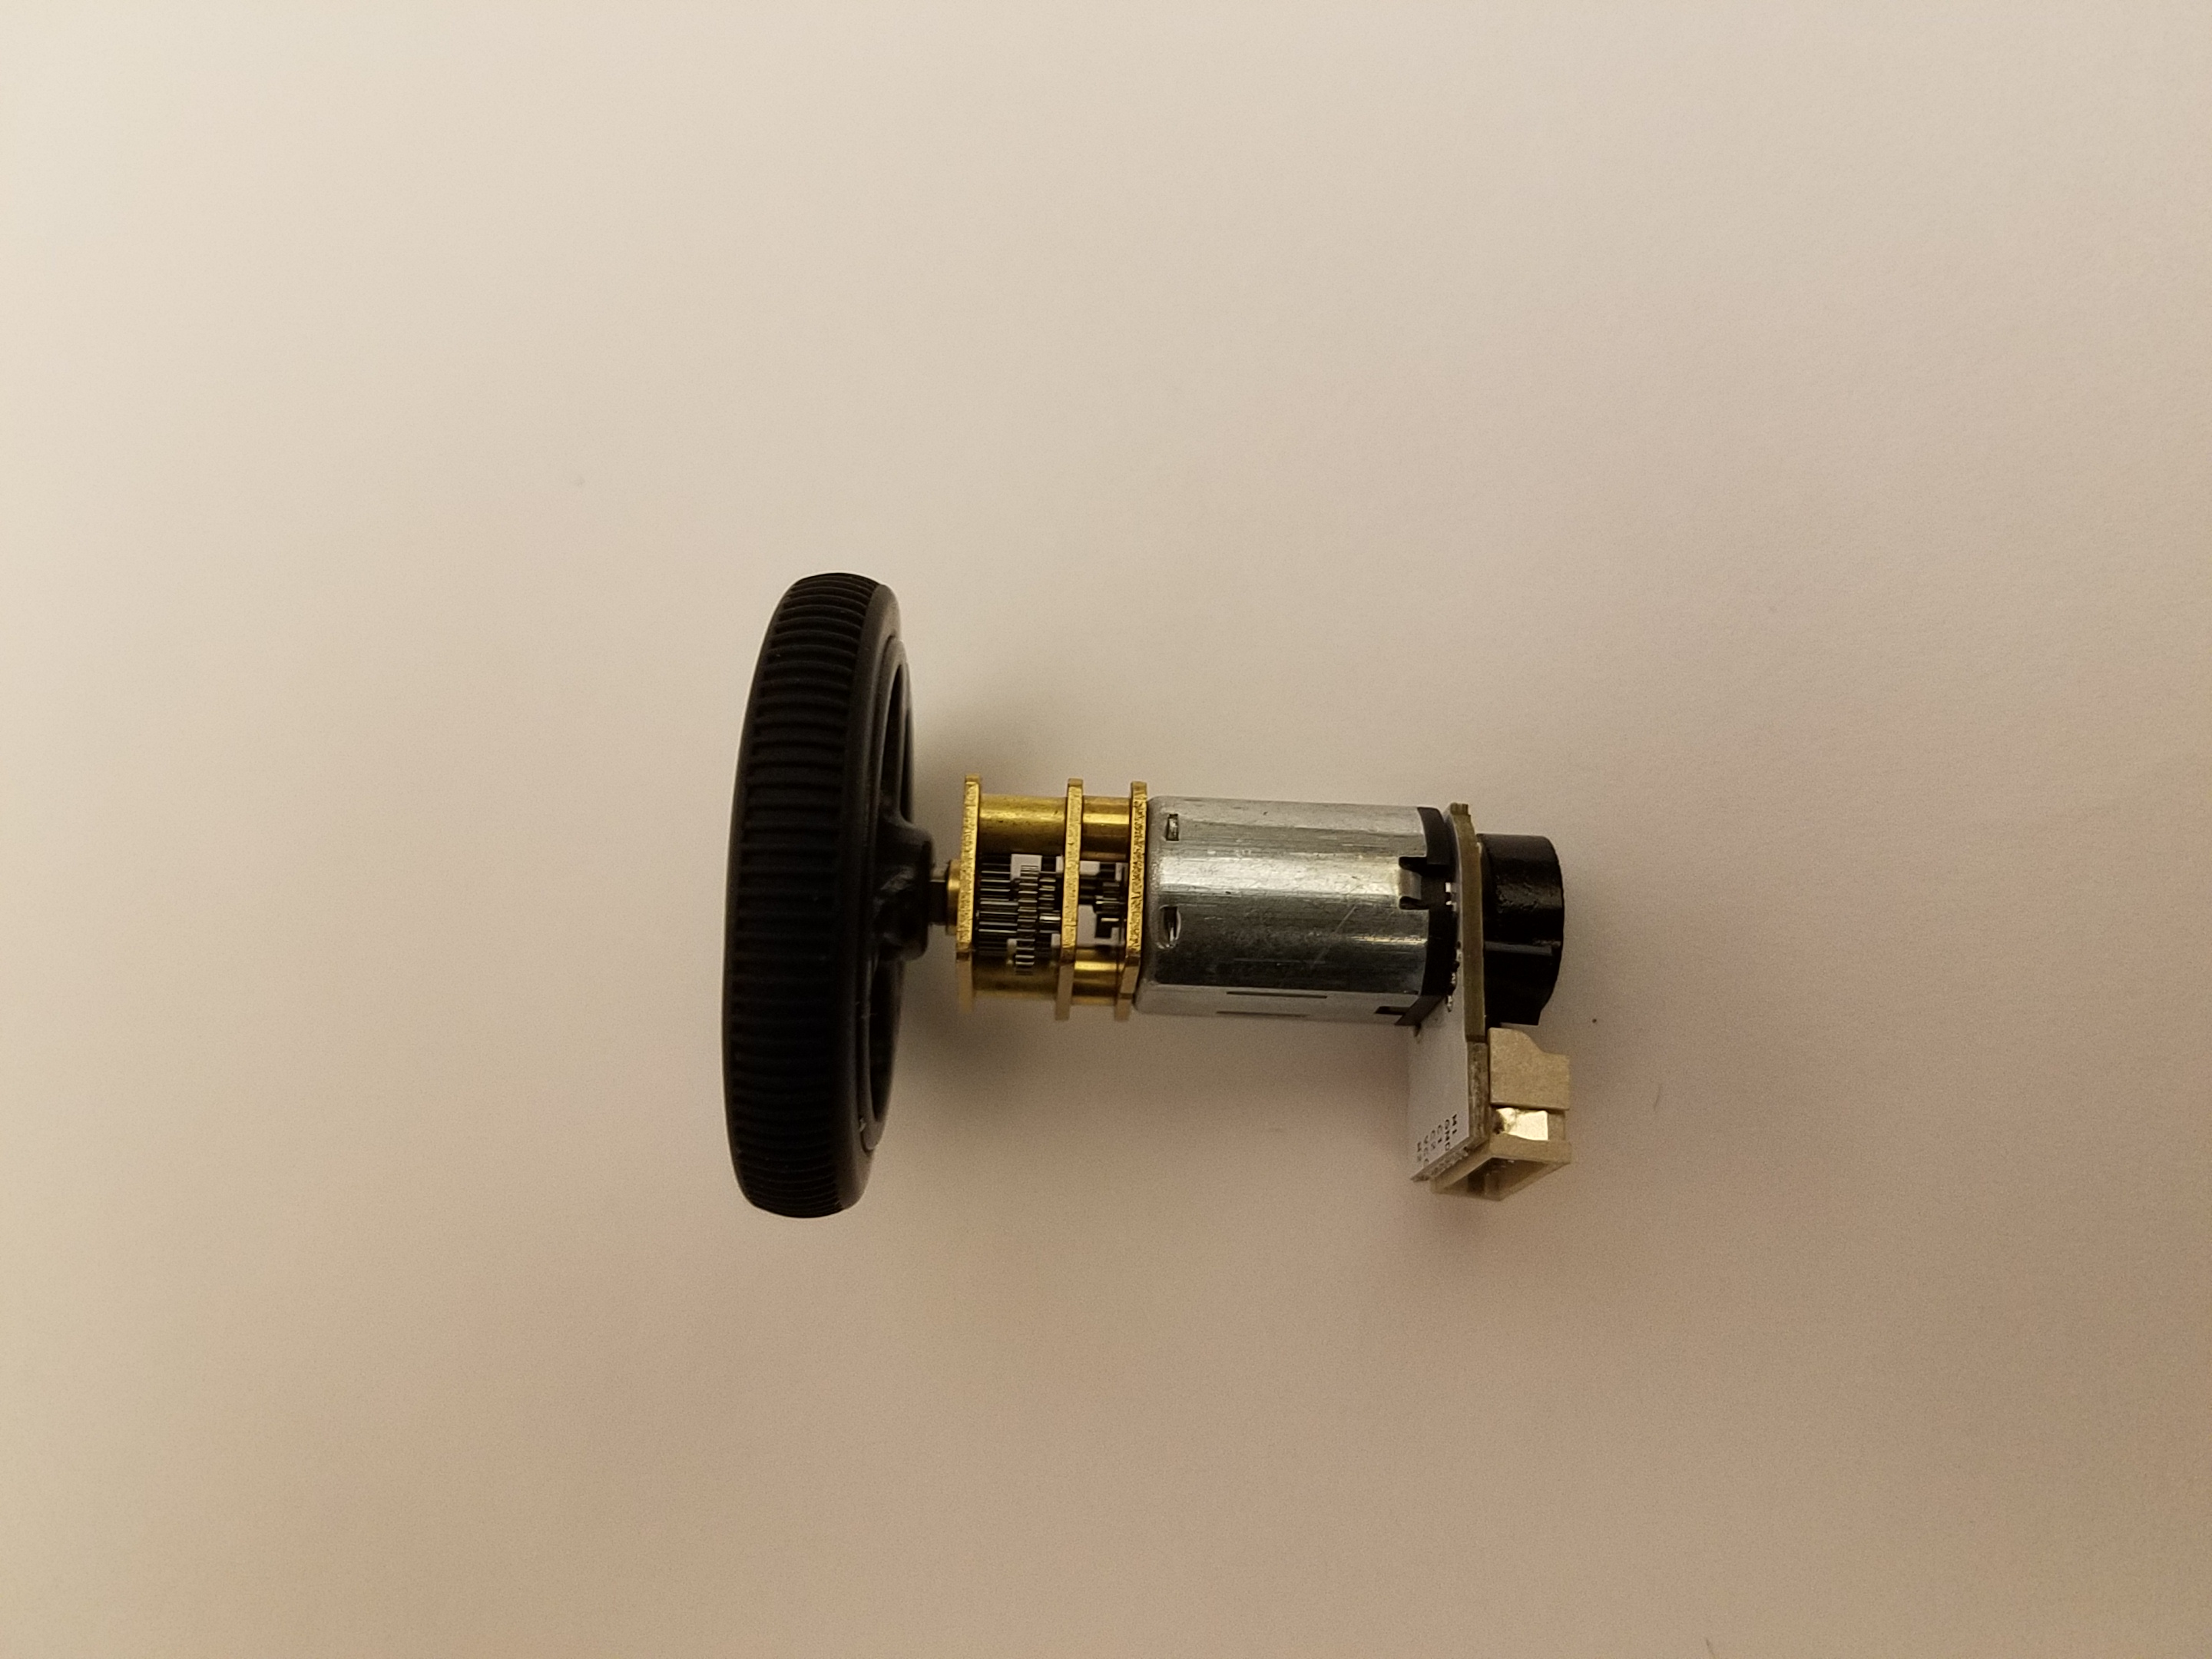
\includegraphics[width=0.45\columnwidth, keepaspectratio]{./figs/20181219_112451.jpg}}\\
\caption{The motor and wheel assembly pressure fit together.}
\label{fig:motorAssembly}
\end{figure}
%End Motor Assembly Picture

\subsubsection{Tamiya Caster Ball Assembly}
\label{sec:casterAssembly}

Since we are dealing with an \emph{differential drive} platform we need an additional, holonomic point of contact to passively stabilize the system. The GRITSBot X uses a Tamiya caster ball assembly with springs that provide a pseudo-suspension for this point of contact. Assembly instructions come with the Tamiya pack but an altered set of instructions will be provided here.

%Caster Parts Picture
\begin{figure}[h!]
\centering
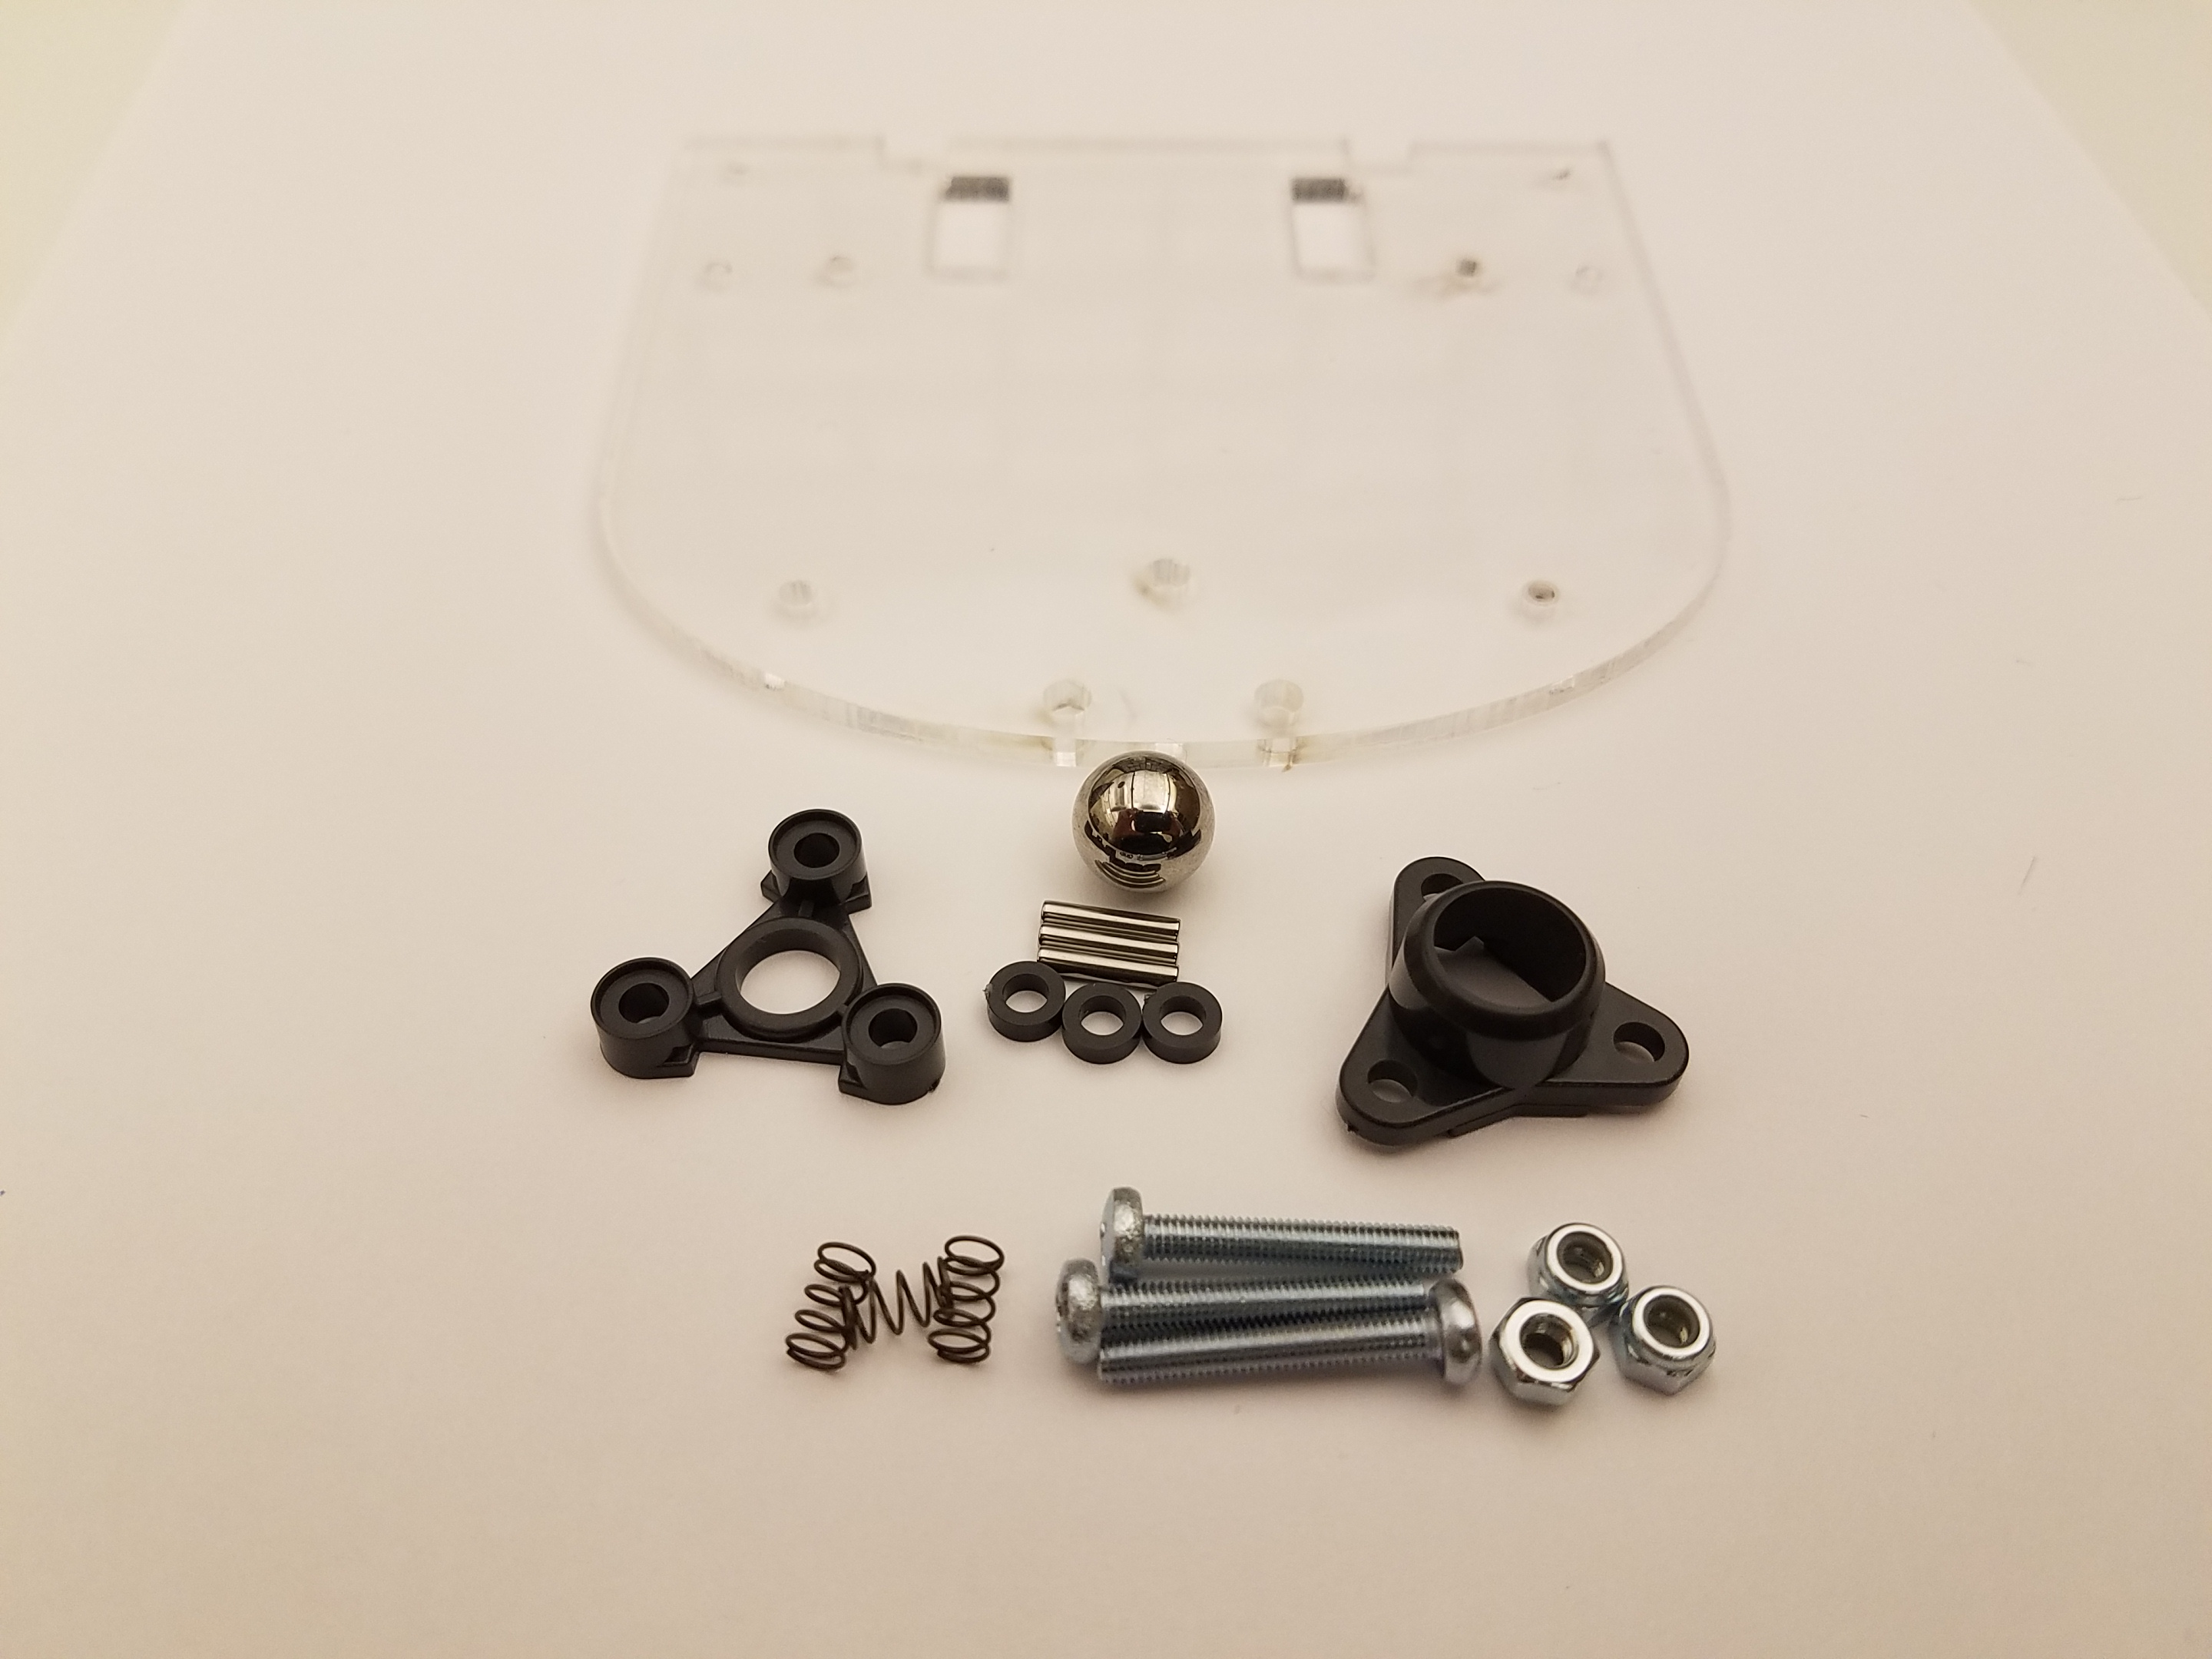
\includegraphics[width=0.65\columnwidth, keepaspectratio]{./figs/20181219_114555.jpg}
\caption{The parts required to construct the caster ball assembly.}
\label{fig:casterParts}
\end{figure}
%End Caster Parts Picture

First, only the parts pictured in \cref{fig:casterParts} are needed. The springs, M3-20 screws, and M3 lock-nuts pictured at the bottom of the figure are not included in the kit. \cref{fig:casterAssembly} shows a picture representation of the assembly steps. A written explanation follows.

%Caster Assembly Picture
\begin{figure}[h!]
\centering
\subfloat[\label{fig:caster1} The caster holder with metal ball and cylindrical bearings inside.]{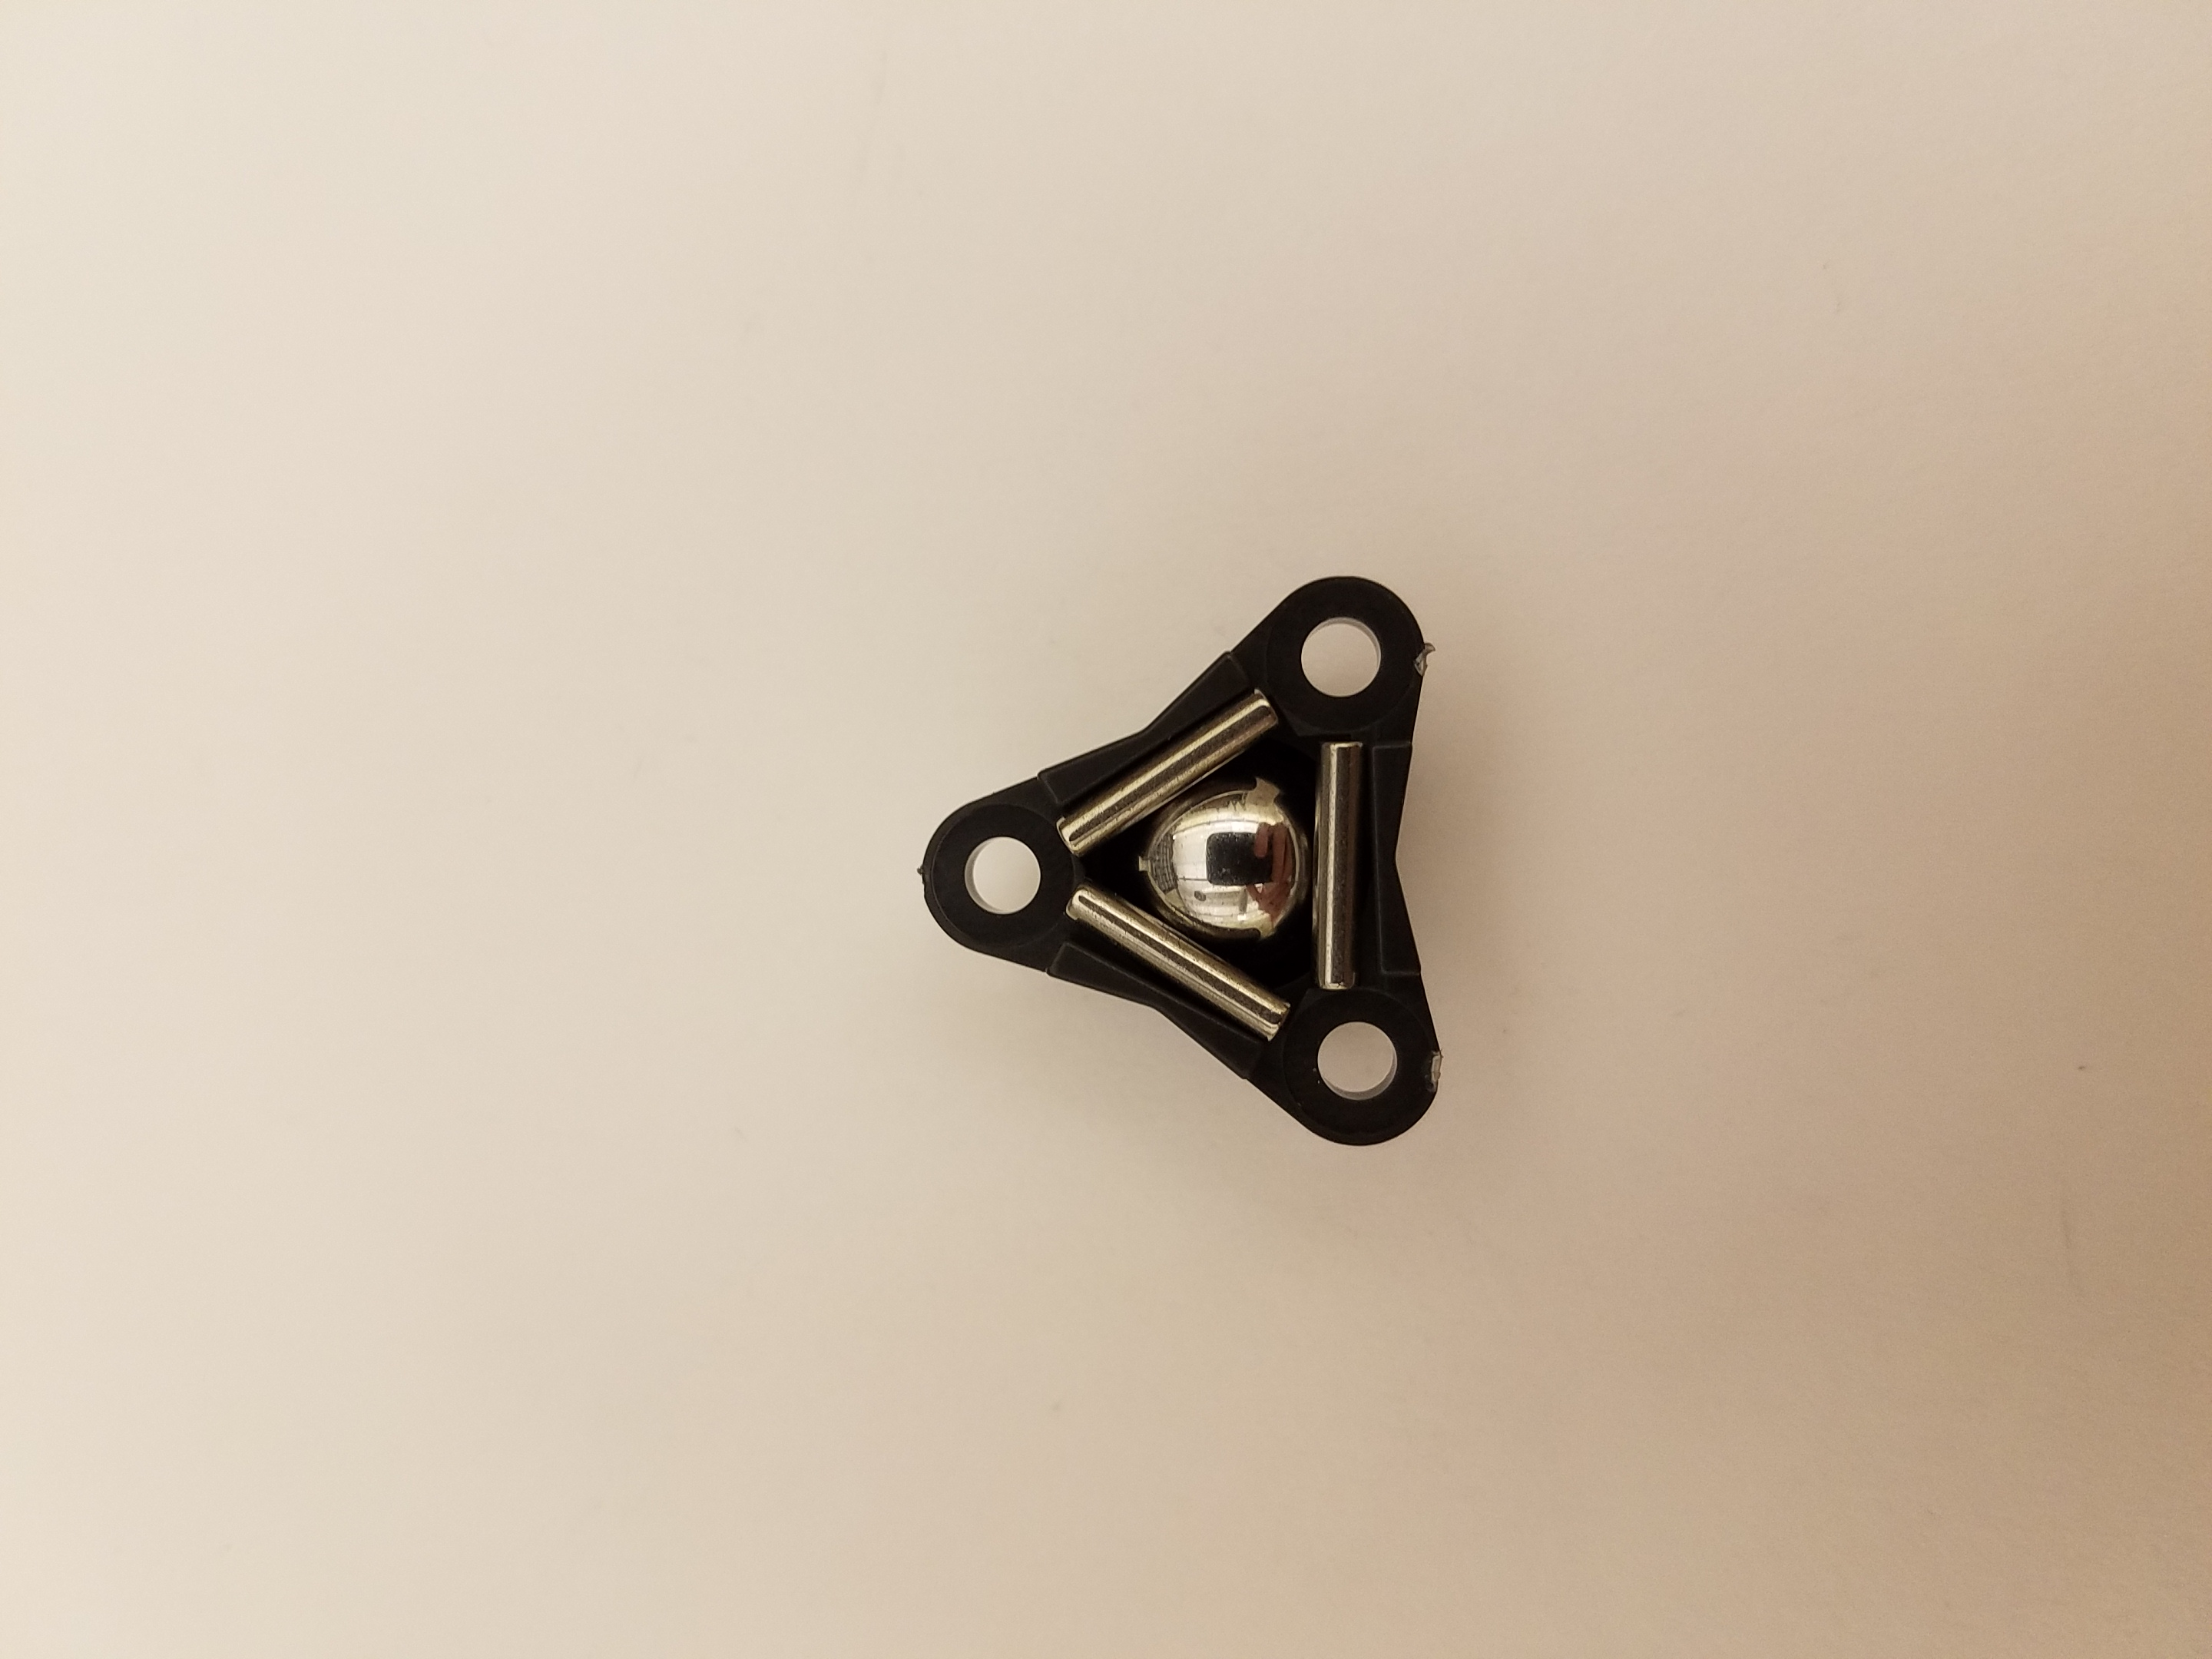
\includegraphics[trim={20cm 0 20cm 0},clip,height=0.45\columnwidth, angle = 270, keepaspectratio]{./figs/20190102_123905.jpg}}
\hfill
\subfloat[\label{fig:caster2} Caster ball assembly with top plate properly inserted.]{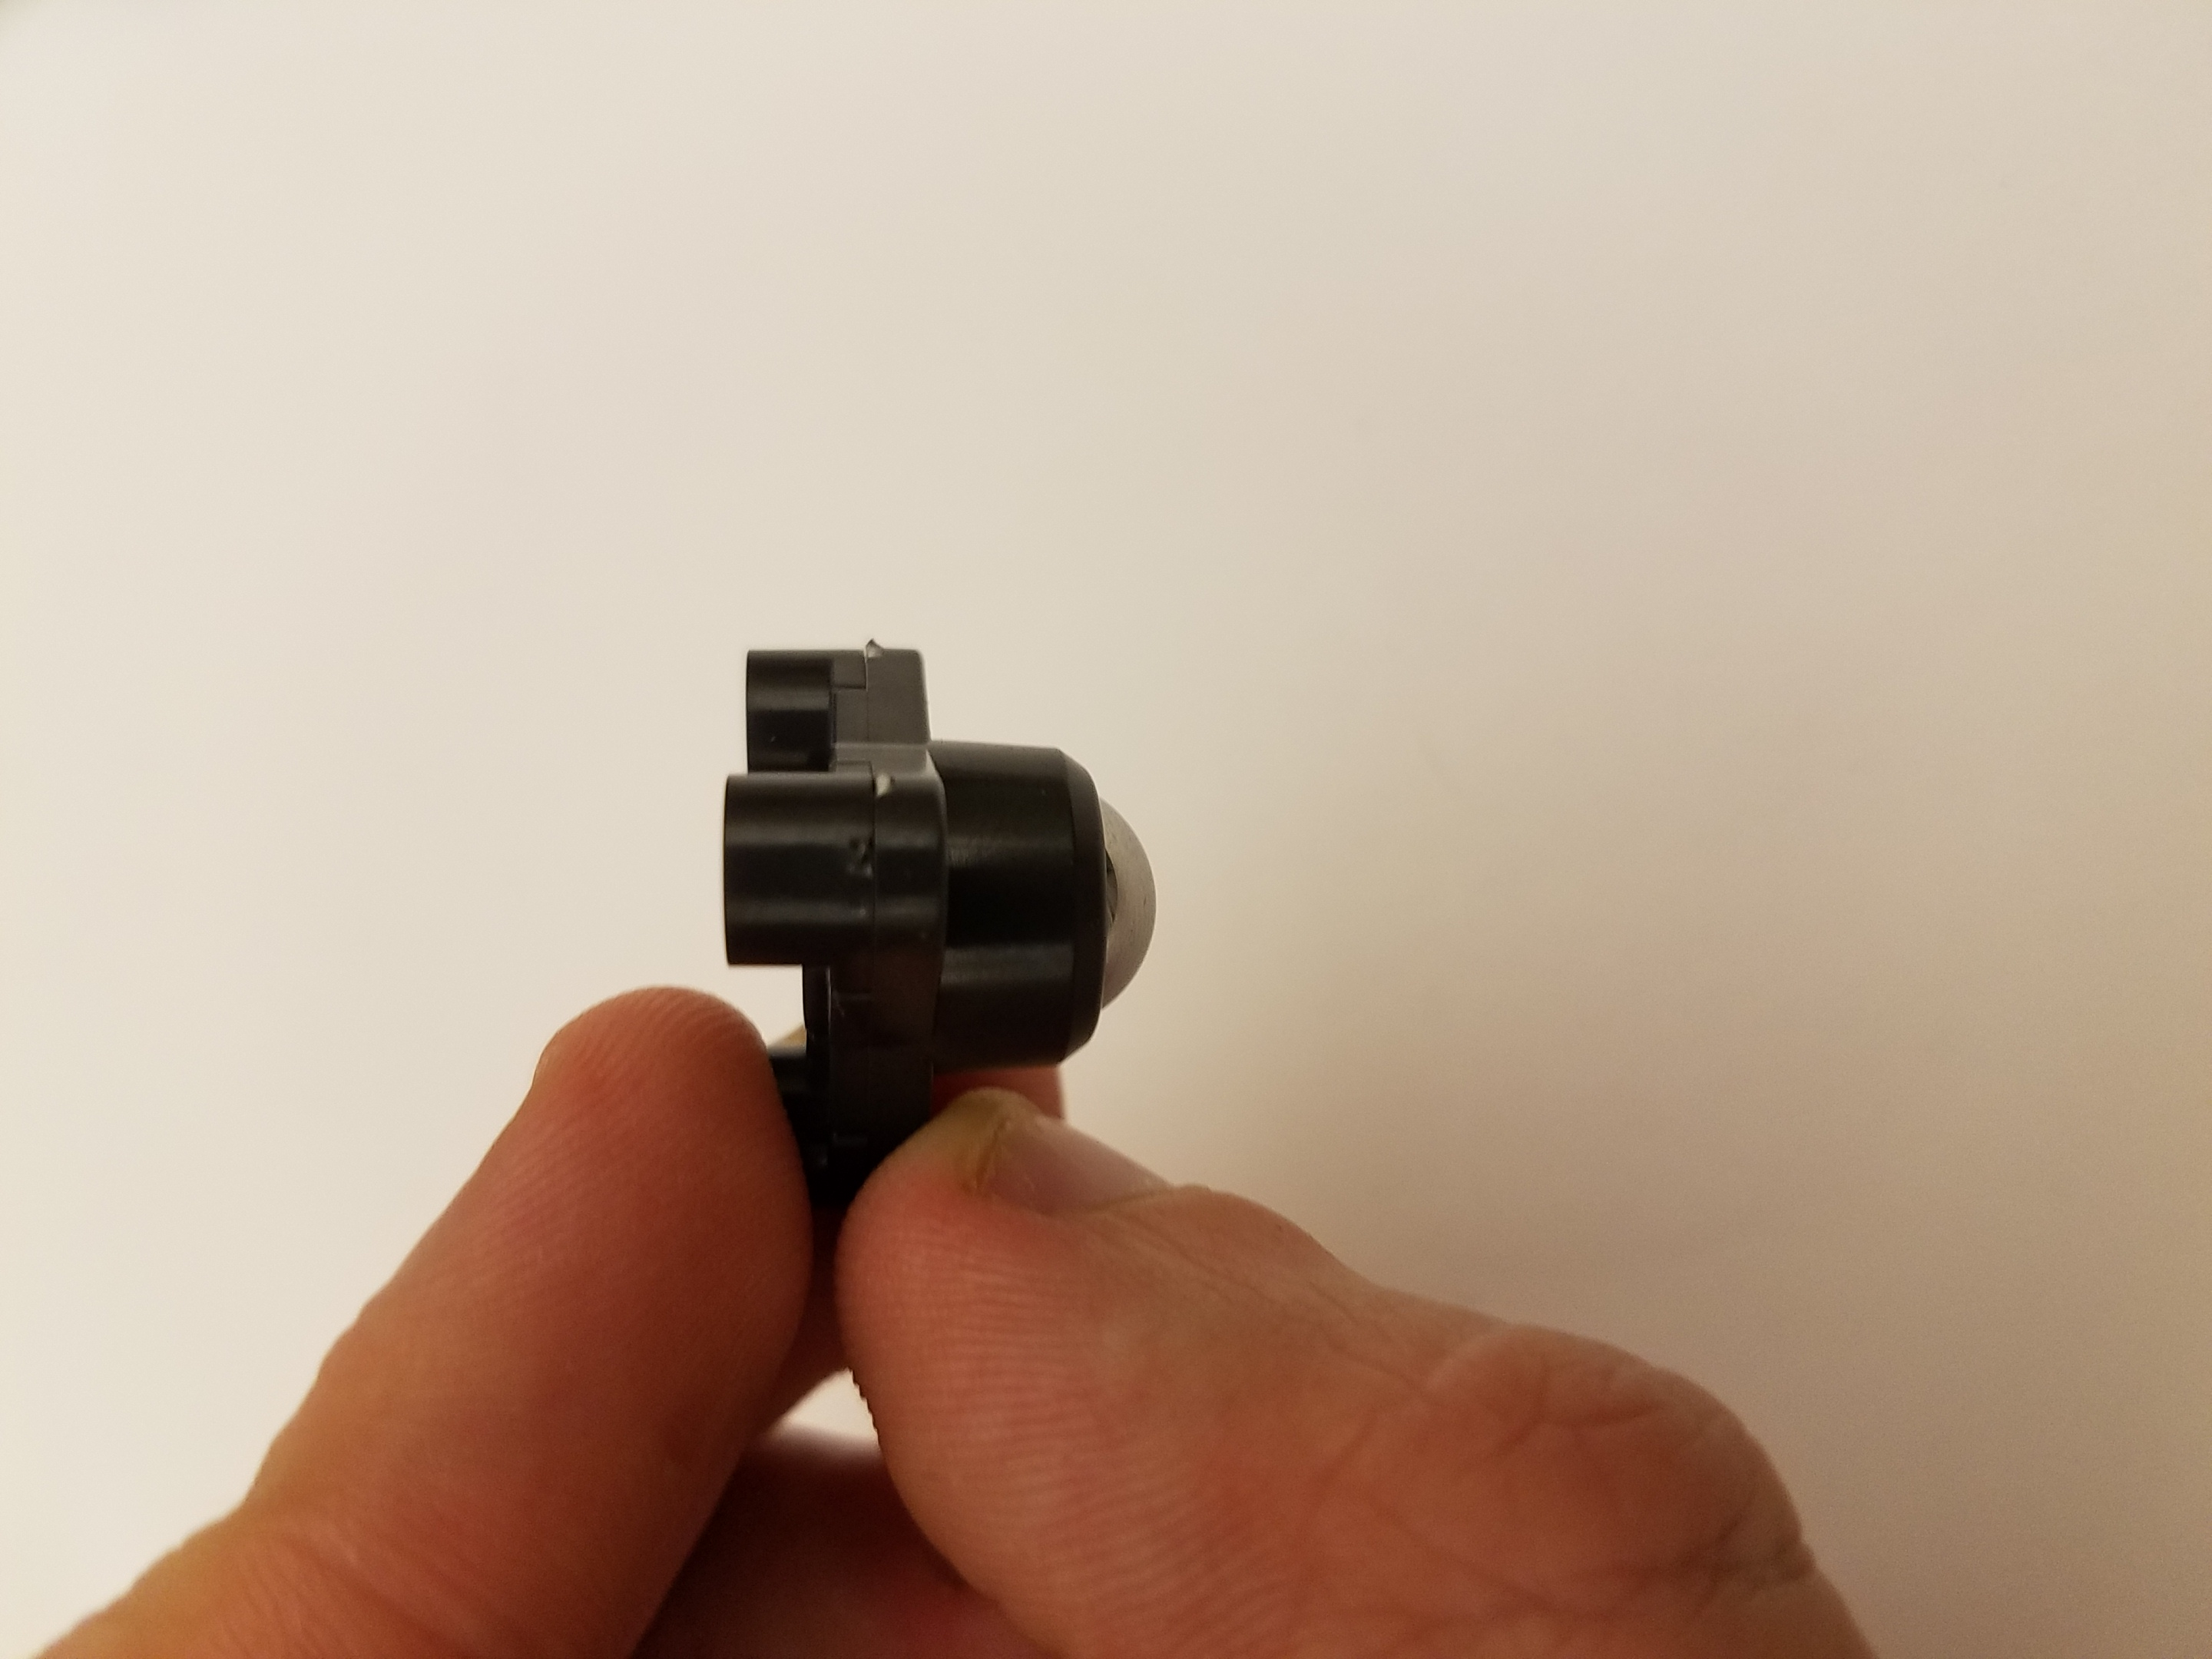
\includegraphics[trim={10cm 0 30cm 0},clip,height=0.45\columnwidth, angle=270, keepaspectratio]{./figs/20190102_123955.jpg}}\\
\subfloat[\label{fig:caster3} Caster assembly with screws, springs, and plastic rings inserted.]{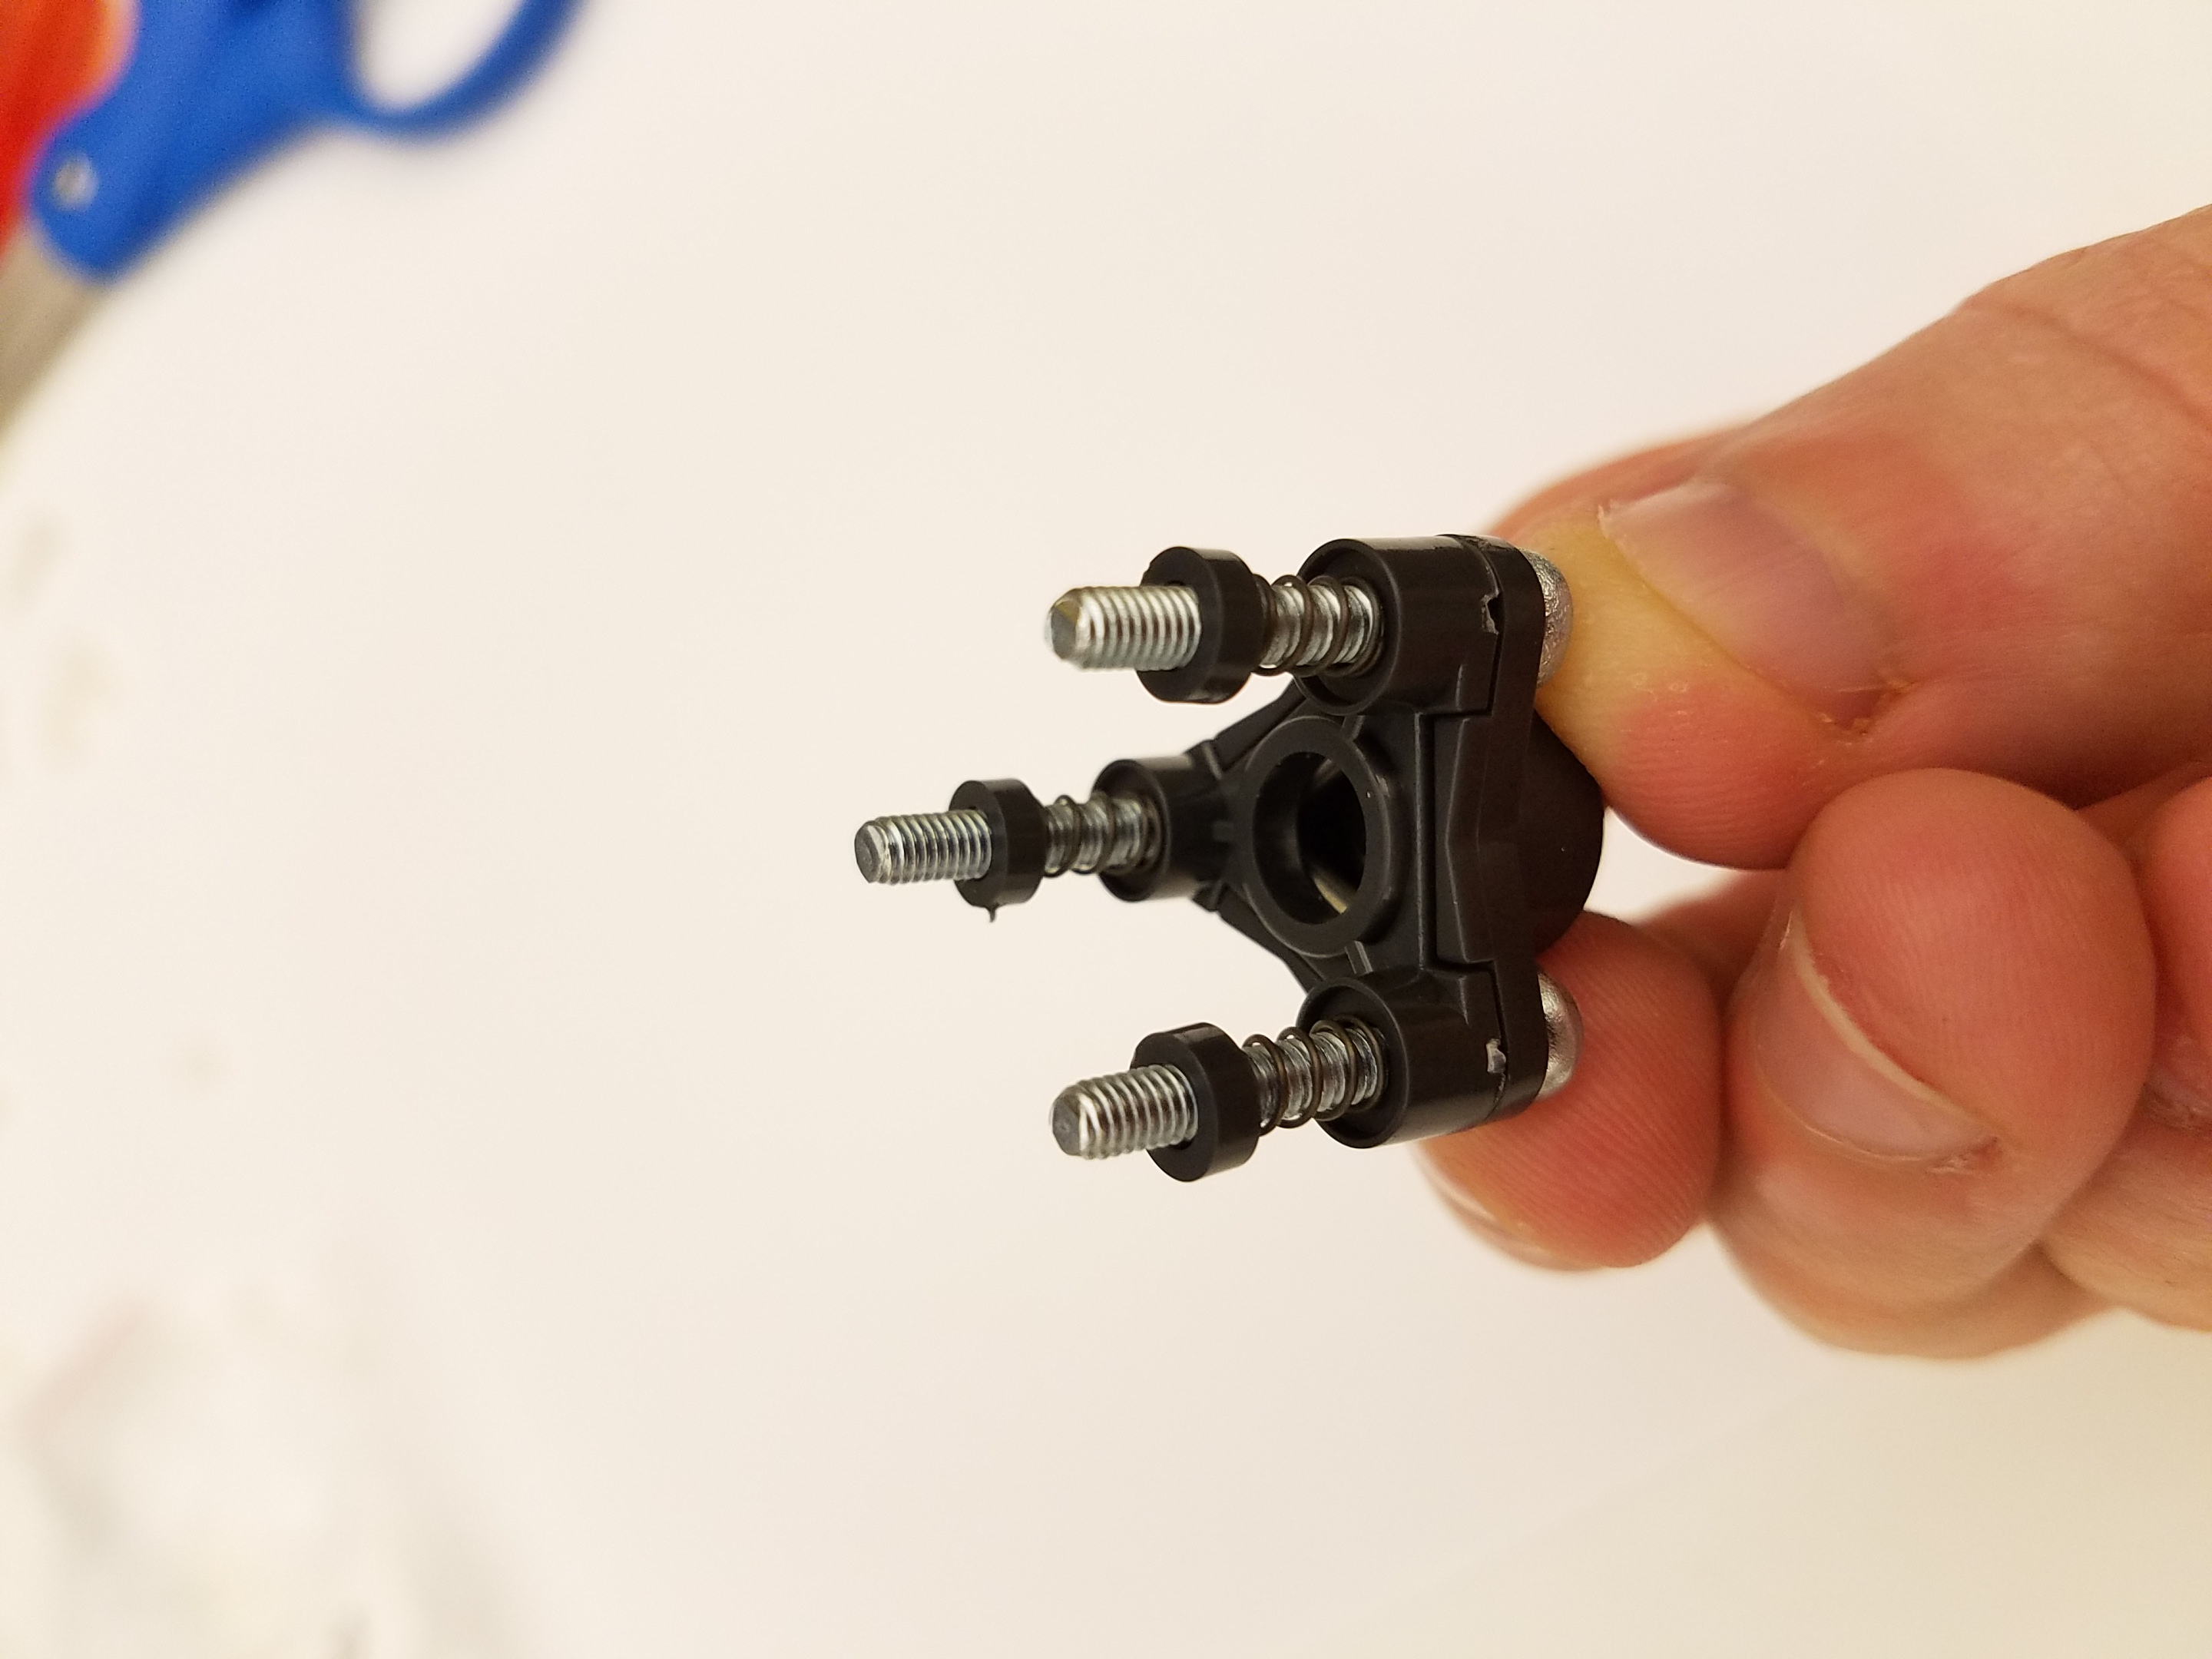
\includegraphics[trim={30cm 0 10cm 0},clip,height=0.45\columnwidth, angle=270, keepaspectratio]{./figs/20190102_124250.jpg}}
\hfill
\subfloat[\label{fig:casterFinished} The finished caster assembly attached to the bottom acrylic plate of the GRITSBot X.]{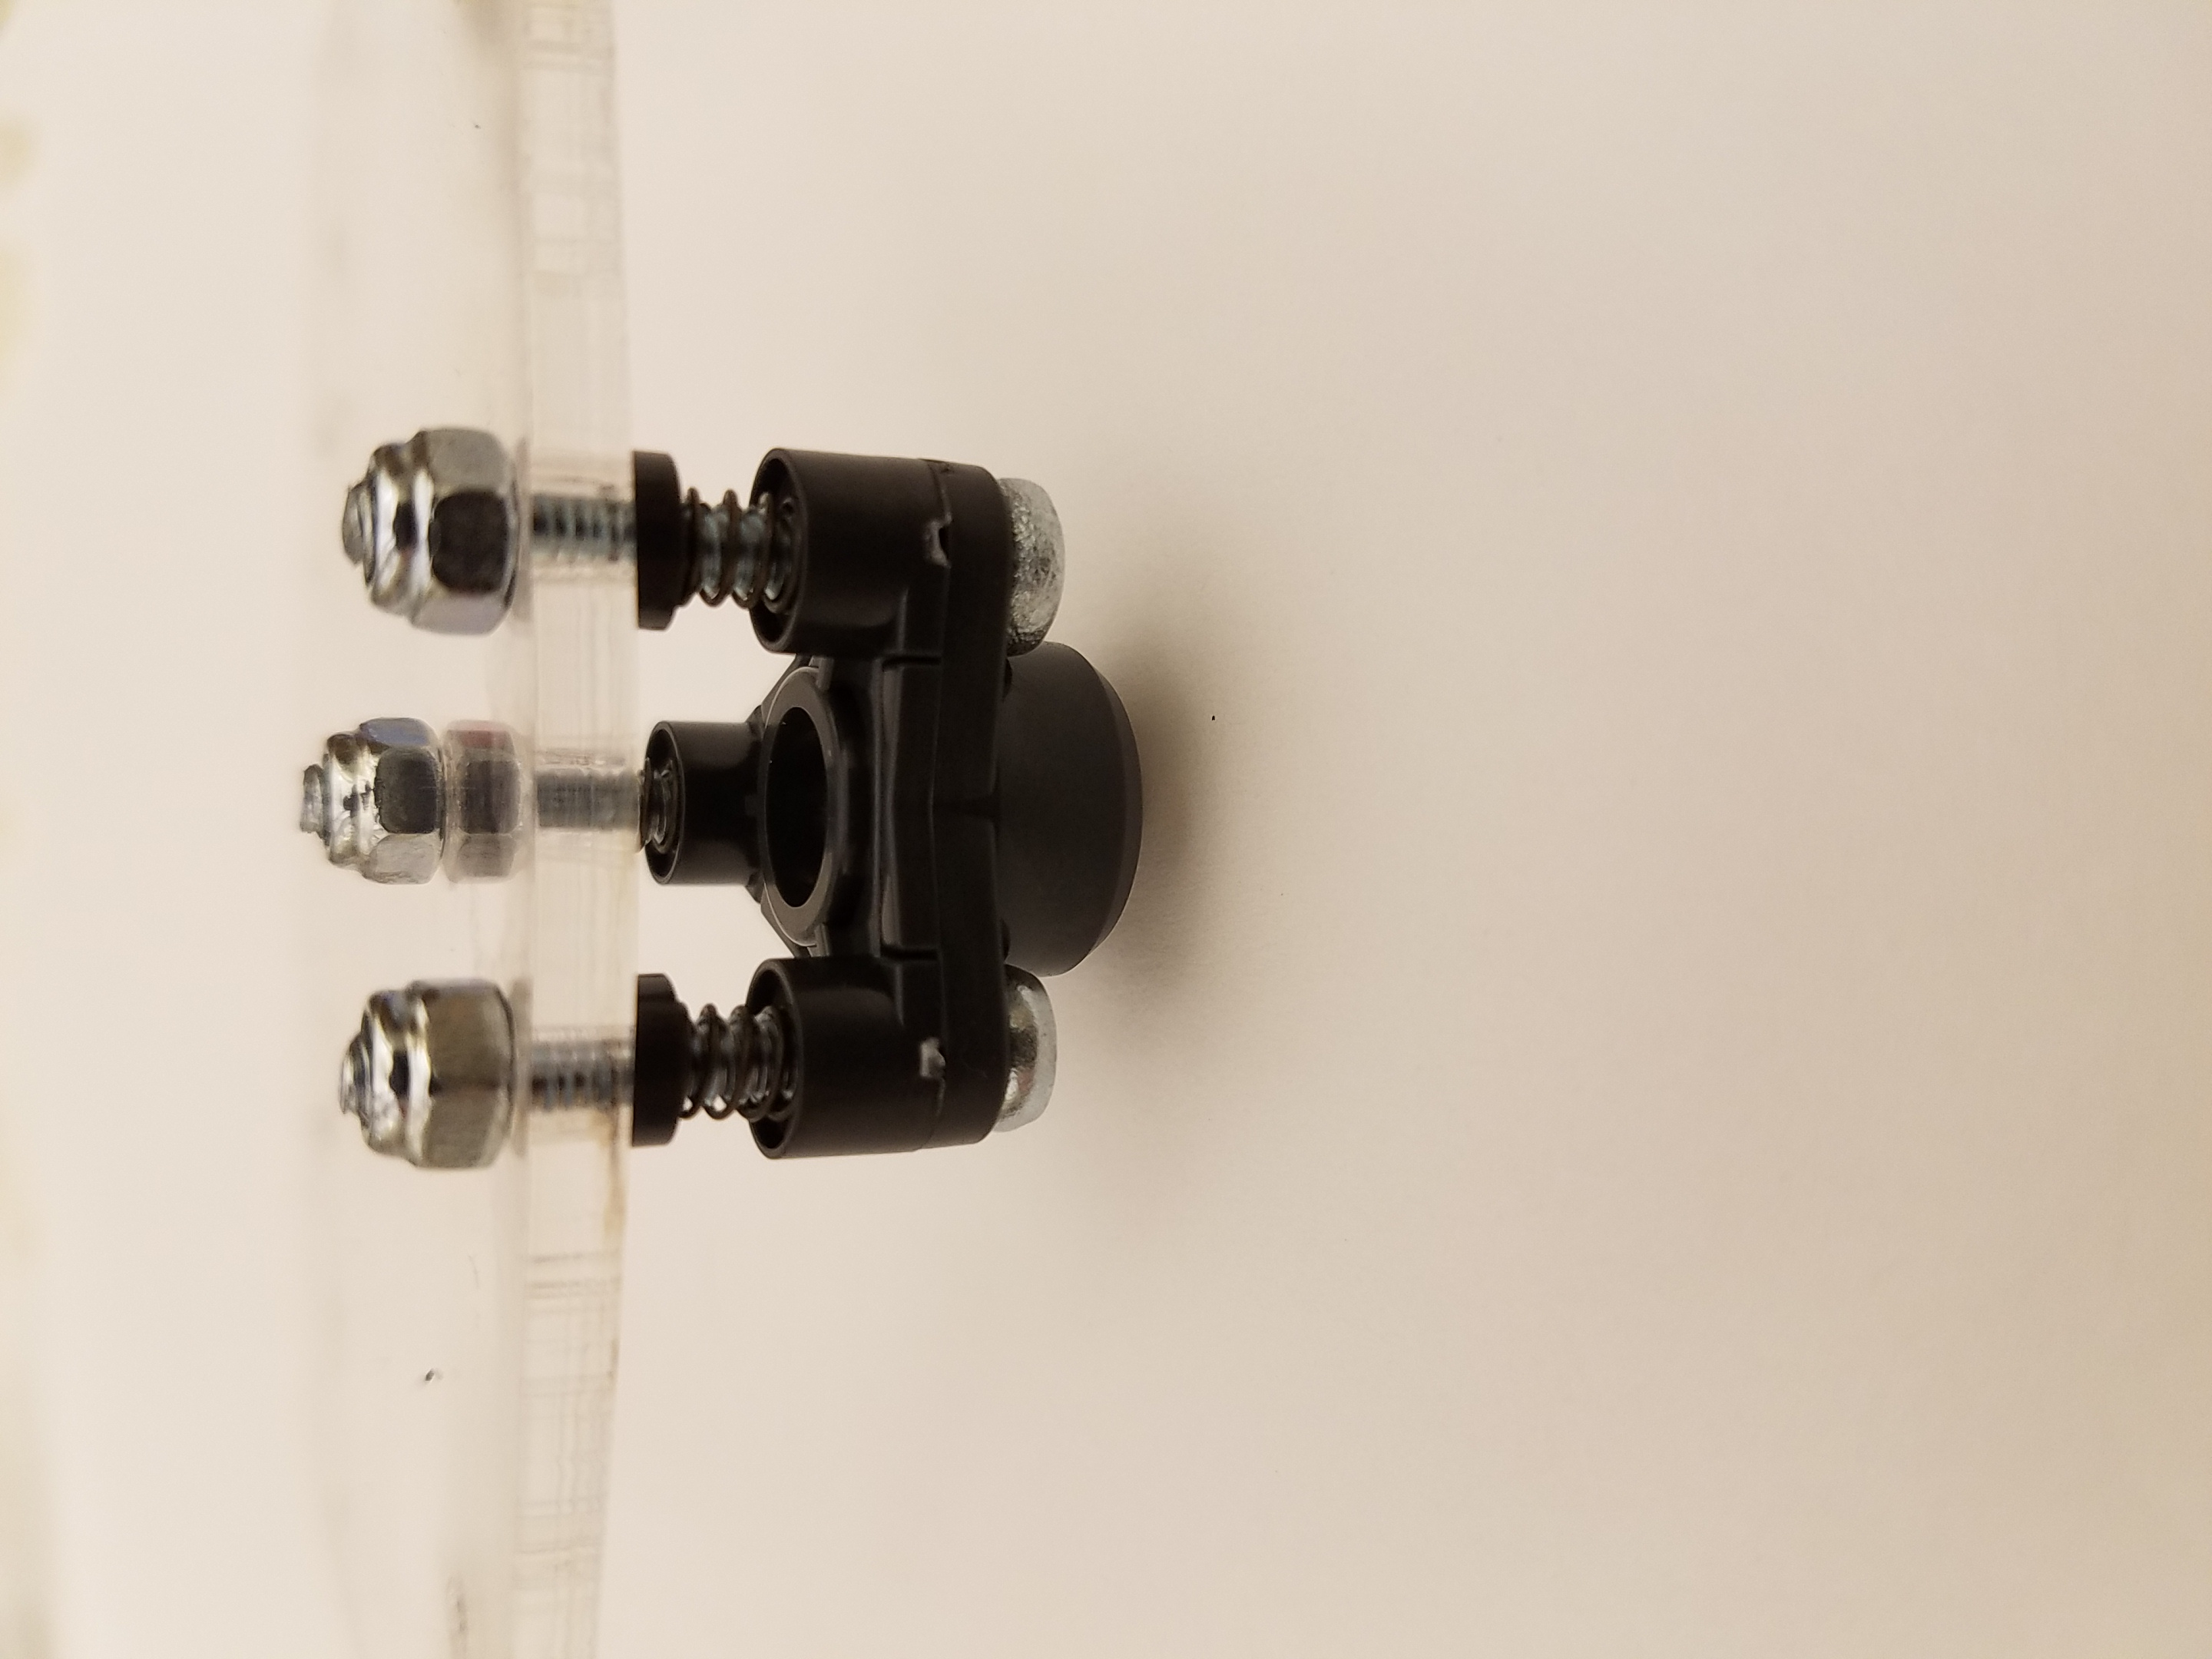
\includegraphics[trim={5cm 0 35cm 0},clip,height=0.45\columnwidth, angle=270, keepaspectratio]{./figs/20190102_124519.jpg}}\\
\caption{Process to put together the caster assembly.}
\label{fig:casterAssembly}
\end{figure}
%End Caster Assembly Picture

First, place the metal ball into the plastic caster shell. Place the three metal cylinders on top of the caster ball such that they fall into the rectangular slots in the plastic as seen in \cref{fig:caster1}. Cover this assembly with the second plastic piece provided by the caster kit. The cover should be placed so the triangle of the cover fits in the cutout of the caster ball holder as seen in \cref{fig:caster2}. There should be no gap between the cover and the caster container. Now that the caster is together, place the three M3 screws through the assembly such that the head of the screw is on the caster ball holder side of the assembly. Place the three springs around the screws. Put the three plastic rings over the springs. The screws with spring and plastic ring assembly should look like \cref{fig:caster3}. Push the screws through the holes of the acrylic base and lock them in place by threading them through the lock nuts. Make sure the screw is deep enough into the lock nut that the assembly will not come apart but not so tight that the spring is extremely compressed. This will be adjusted once the wheels are on to level the base.

If done correctly, the assembly should look like \cref{fig:casterFinished}. Test to make sure the caster is free moving by running your hand along the ball. It should move freely. If it doesn't, it's possible one of the metal cylinders came loose during assembly and is restricting the motion. If this is the case, the caster must be reassembled.

\subsubsection{Attaching the Motors and Caster to the Base Plate}
\label{sec:baseAssembly}

Finally, attach the motors to the base of the chassis. This is done by placing the motor bracket over the exposed gear box of the micro-metal gear motor as seen in \cref{fig:bracketMotor}. Note the plastic motor bracket has a rounded and rectangular surface as seen in \cref{fig:bracketDifference}. 

%Motor Bracket Picture
\begin{figure}[h!]
\centering
\subfloat[\label{fig:bracketDifference}  The rectangular opening (left) and curved opening (right) of the motor mounting brackets.]{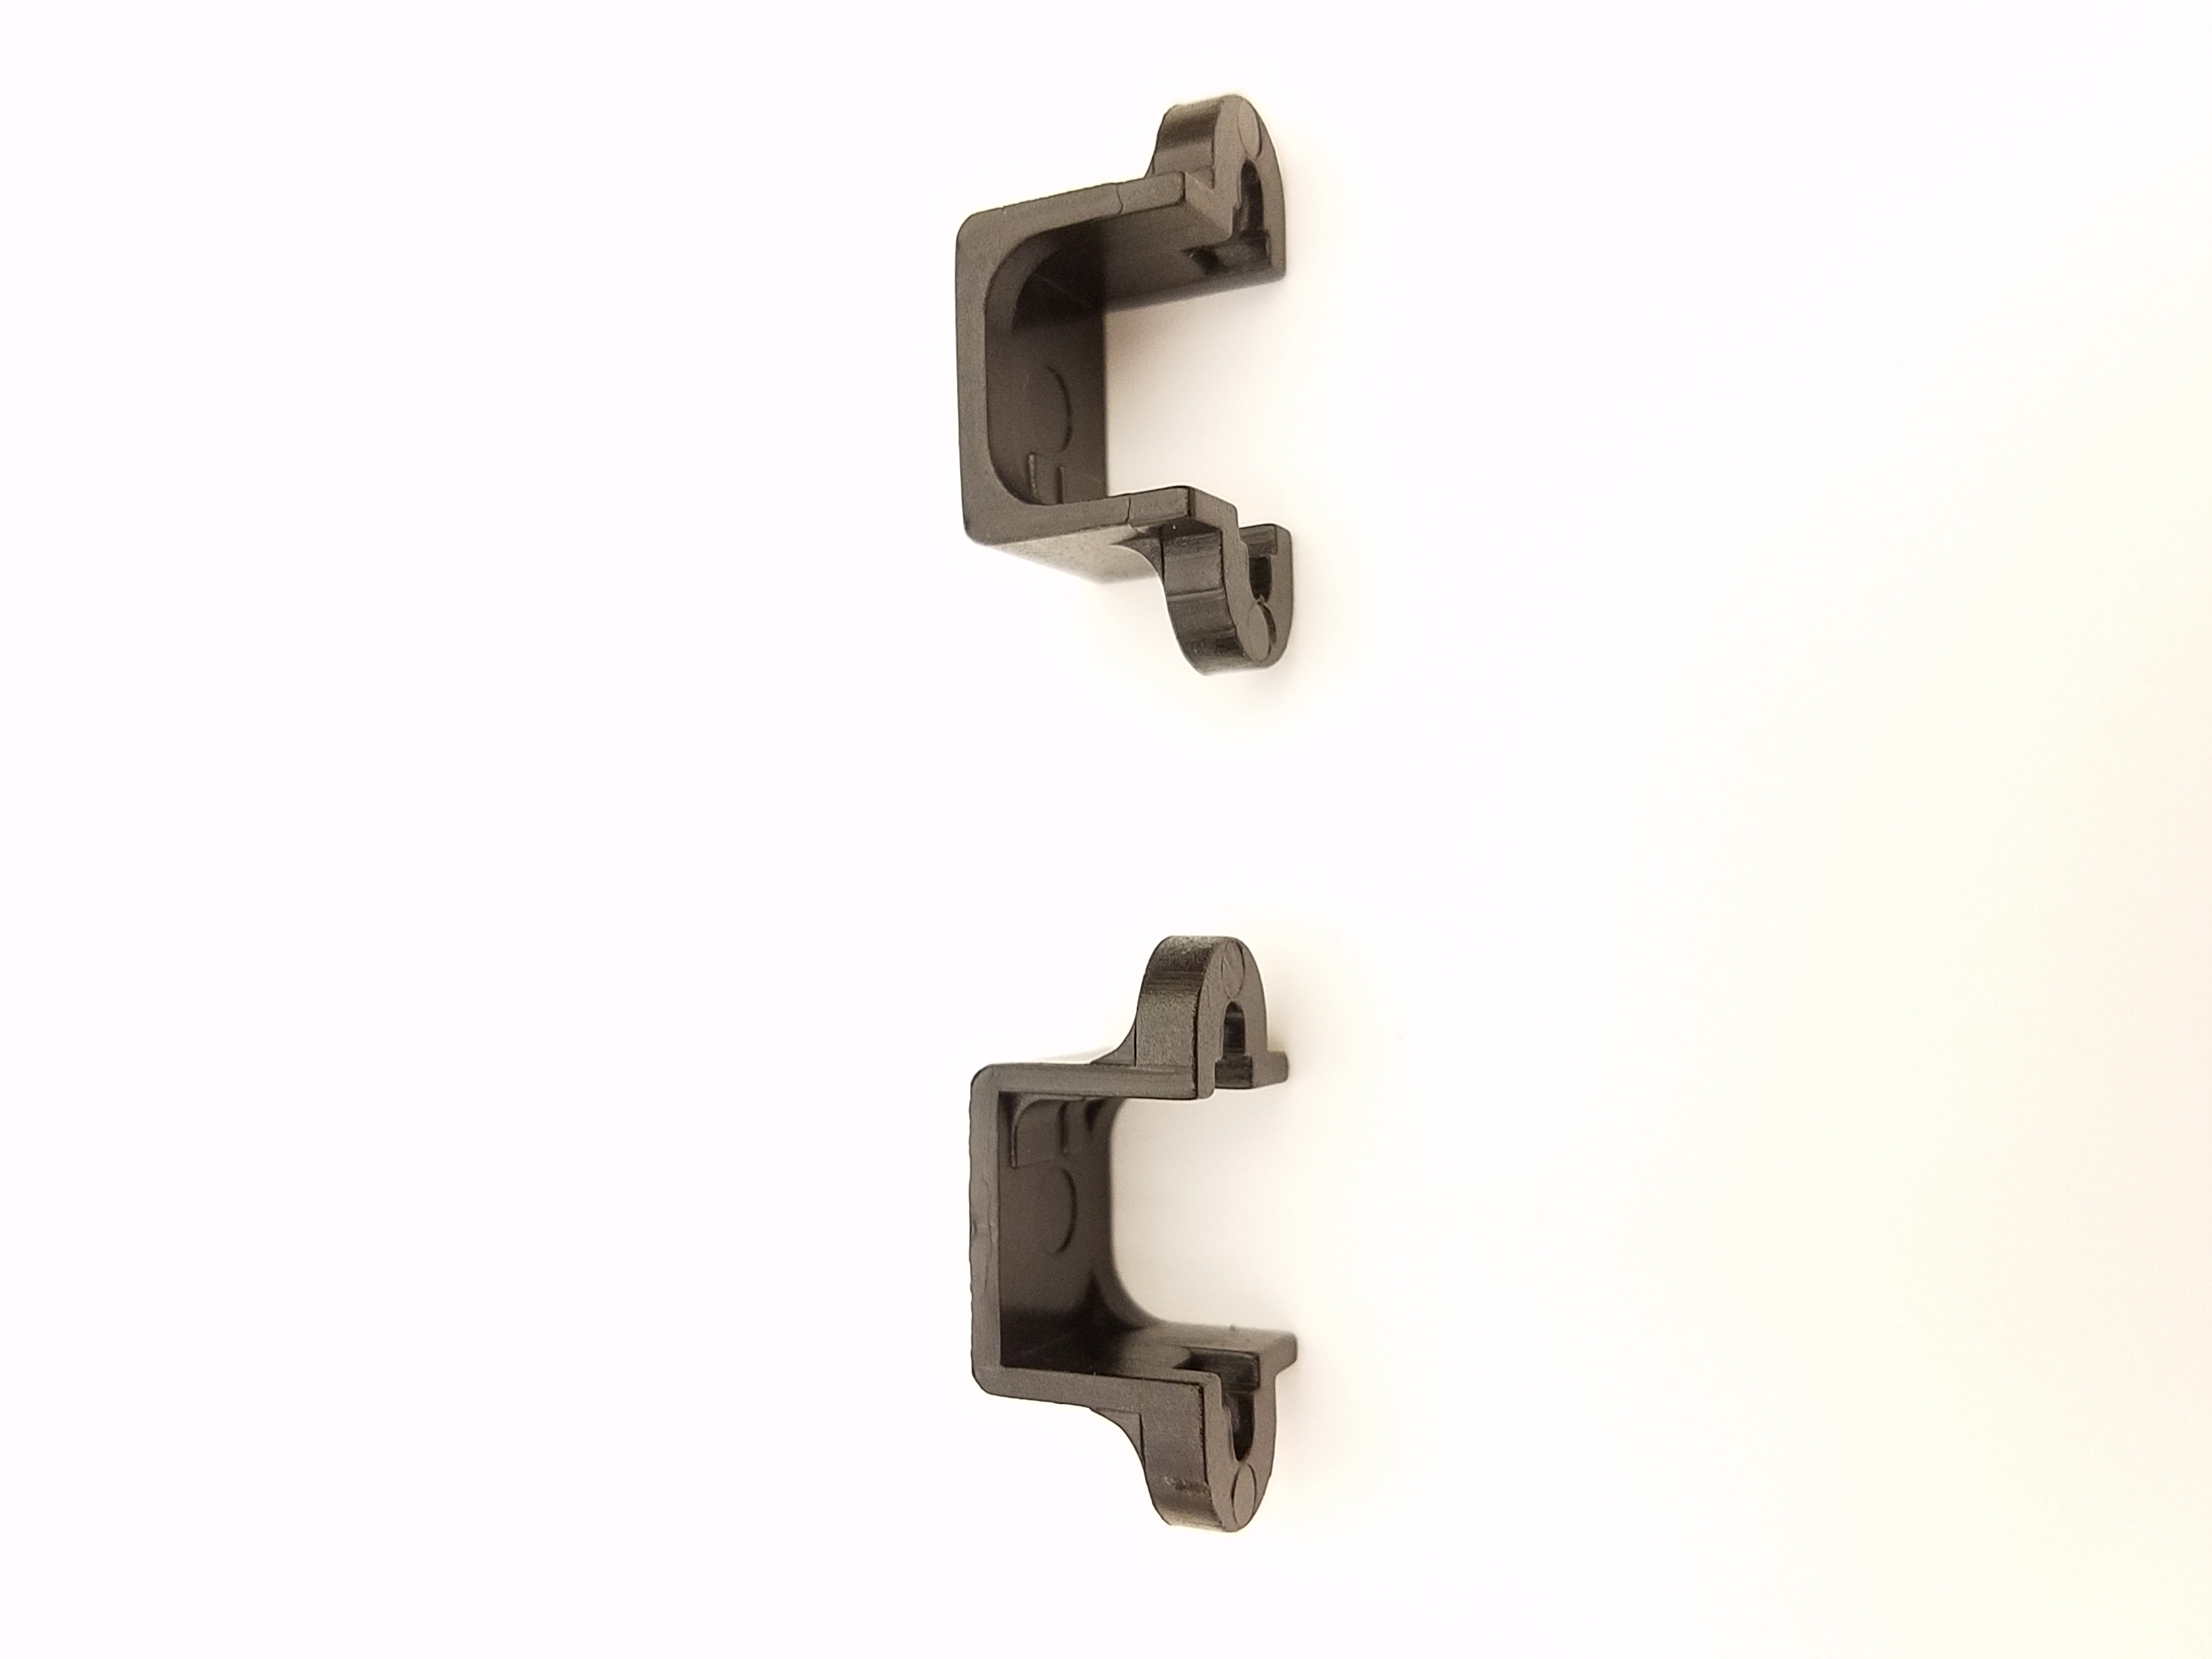
\includegraphics[width=0.45\columnwidth, keepaspectratio]{./figs/20190102_124735.jpg}}
\hfill
\subfloat[\label{fig:bracketMotor} Brackets properly attached to the micro metal gear motors.]{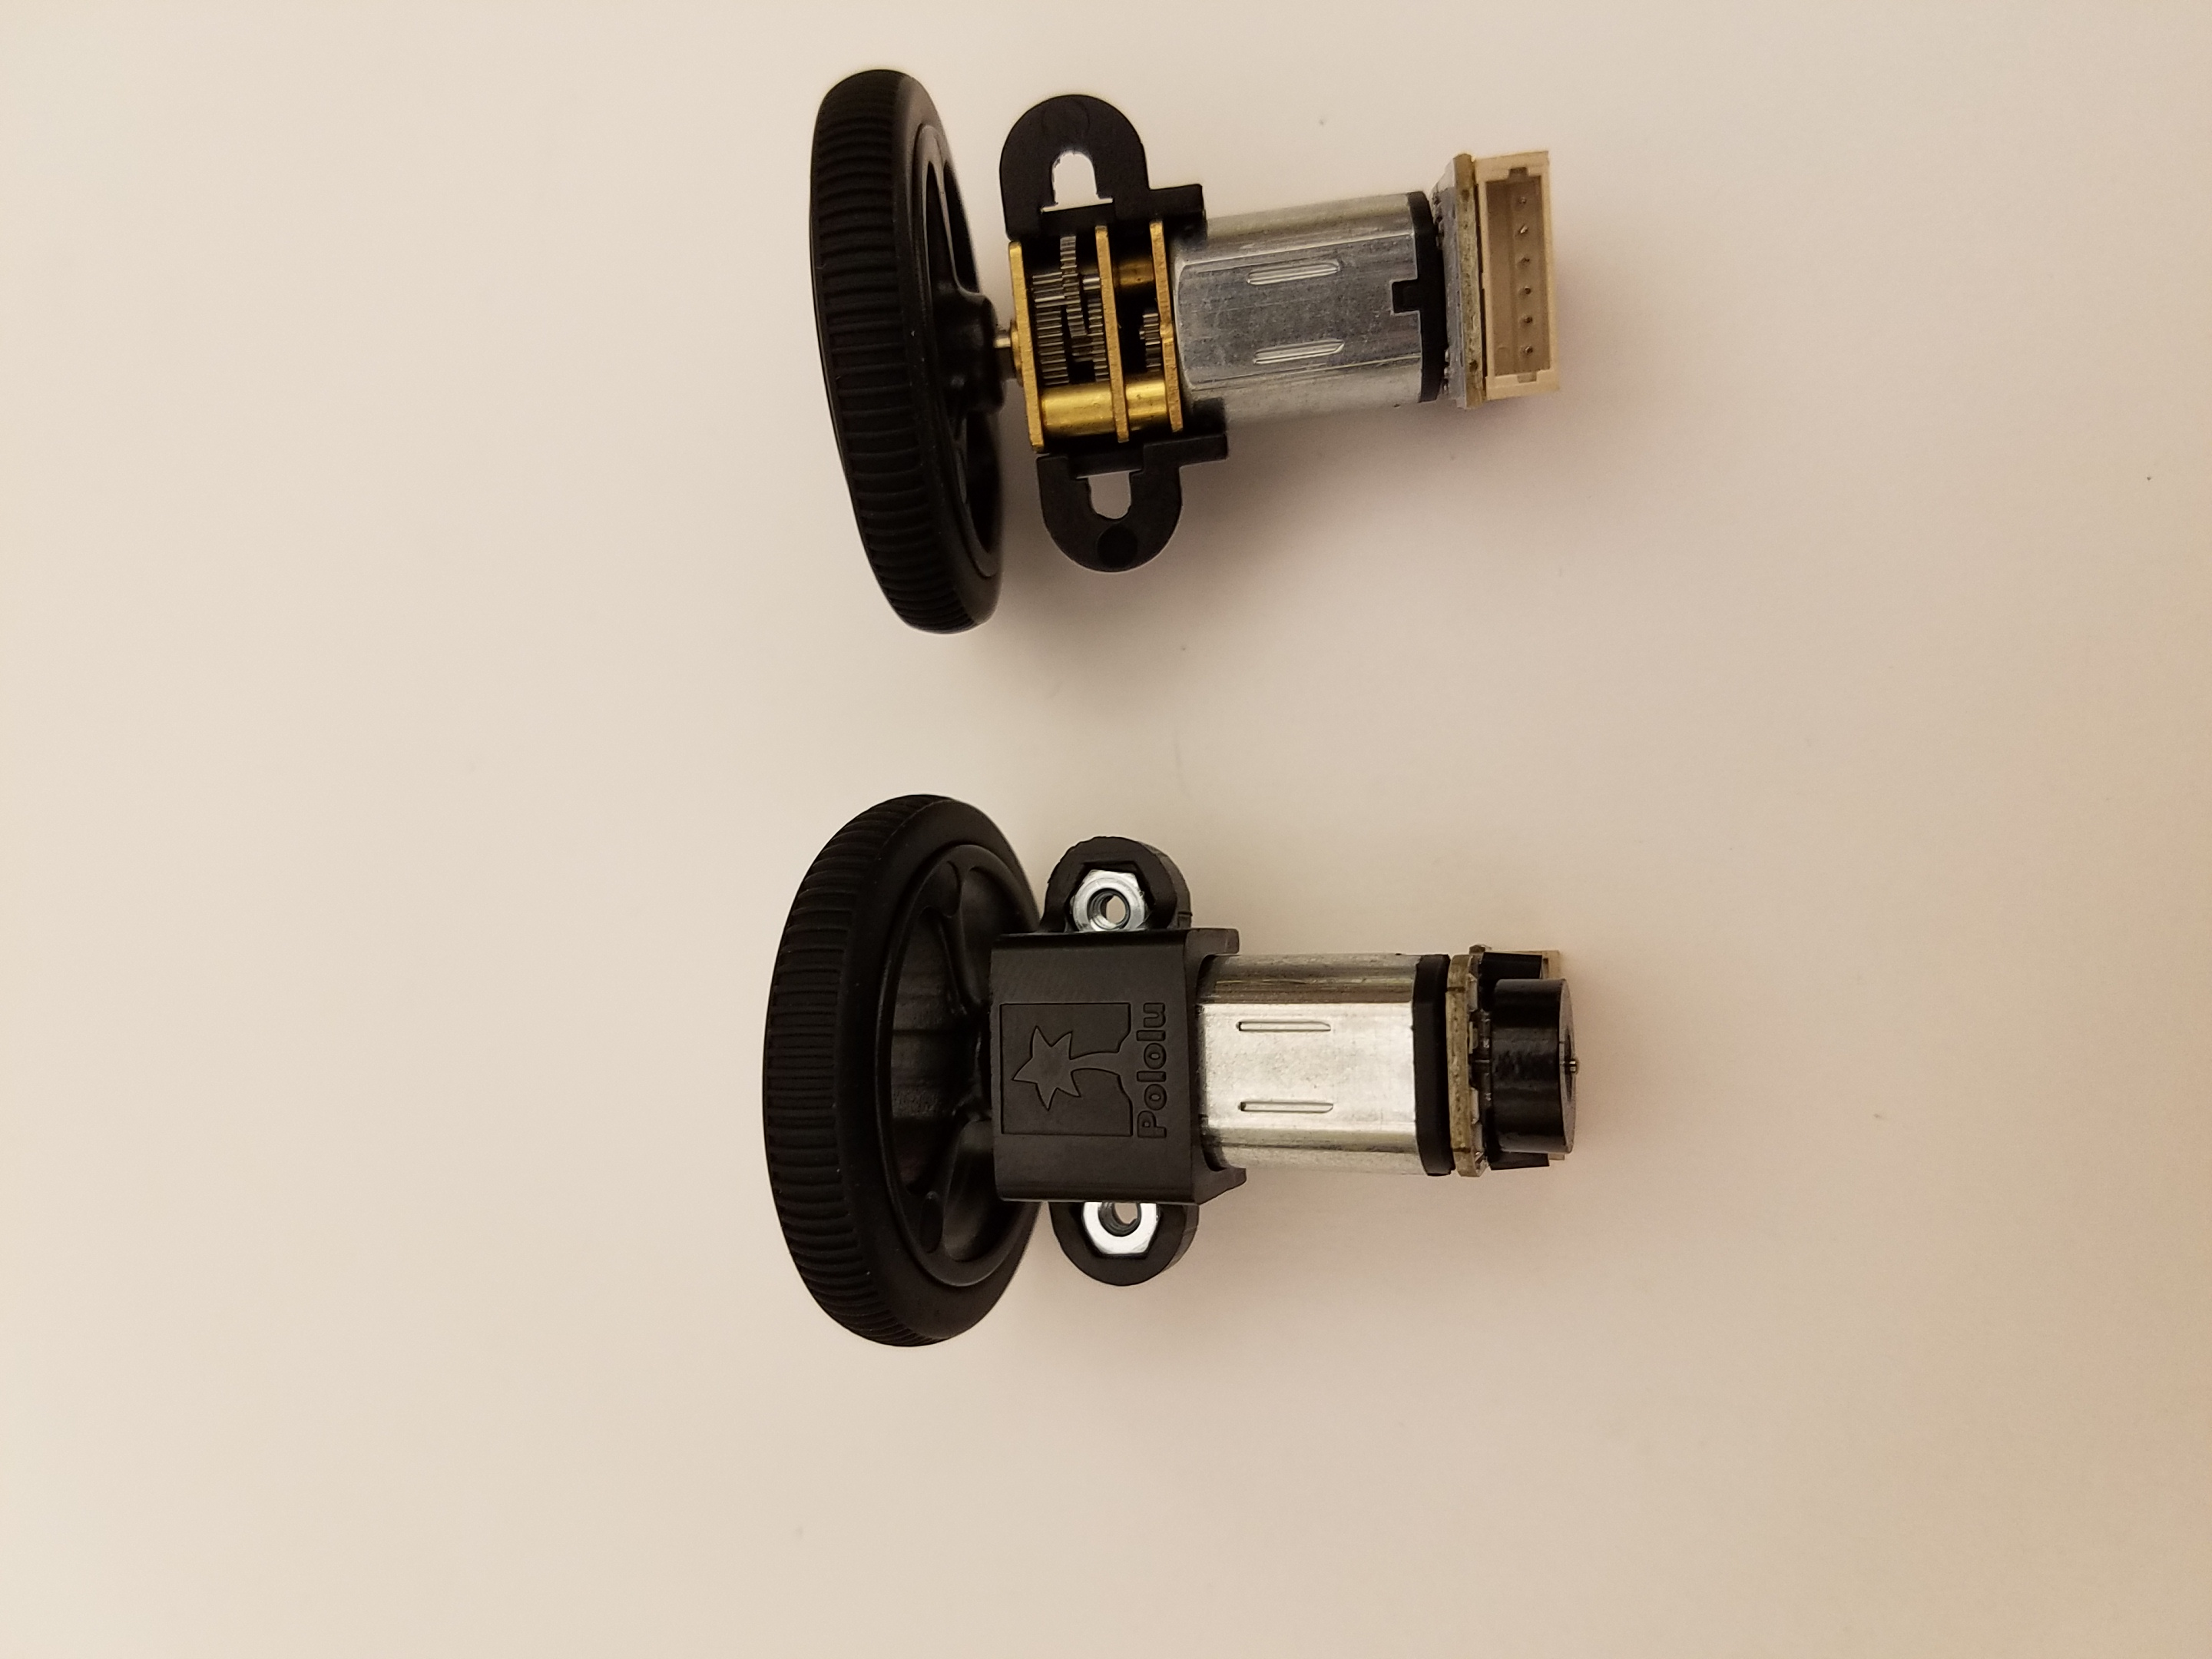
\includegraphics[width=0.45\columnwidth, keepaspectratio]{./figs/20190102_125013.jpg}}\\
\caption{Attaching the brackets to the micro-metal gear motors properly.}
\label{fig:properMotorBracket}
\end{figure}
%End Motor Bracket Picture

Make sure the rounded surface rests on the hull of the motor and the rectangular surface rests on the gear box. This motor bracket should be put onto the motor such that the open side is on the same side as the motor connections for the encoder. Place the nut into the hexogonal space on the bracket and thread the screw through the acrylic into the motor bracket. Tighten the caster nuts as appropriate to make the chassis base as level as possible. The final assembly should look like \cref{fig:finalBase}.

%Finished Base Picture
\begin{figure}[h!]
\centering
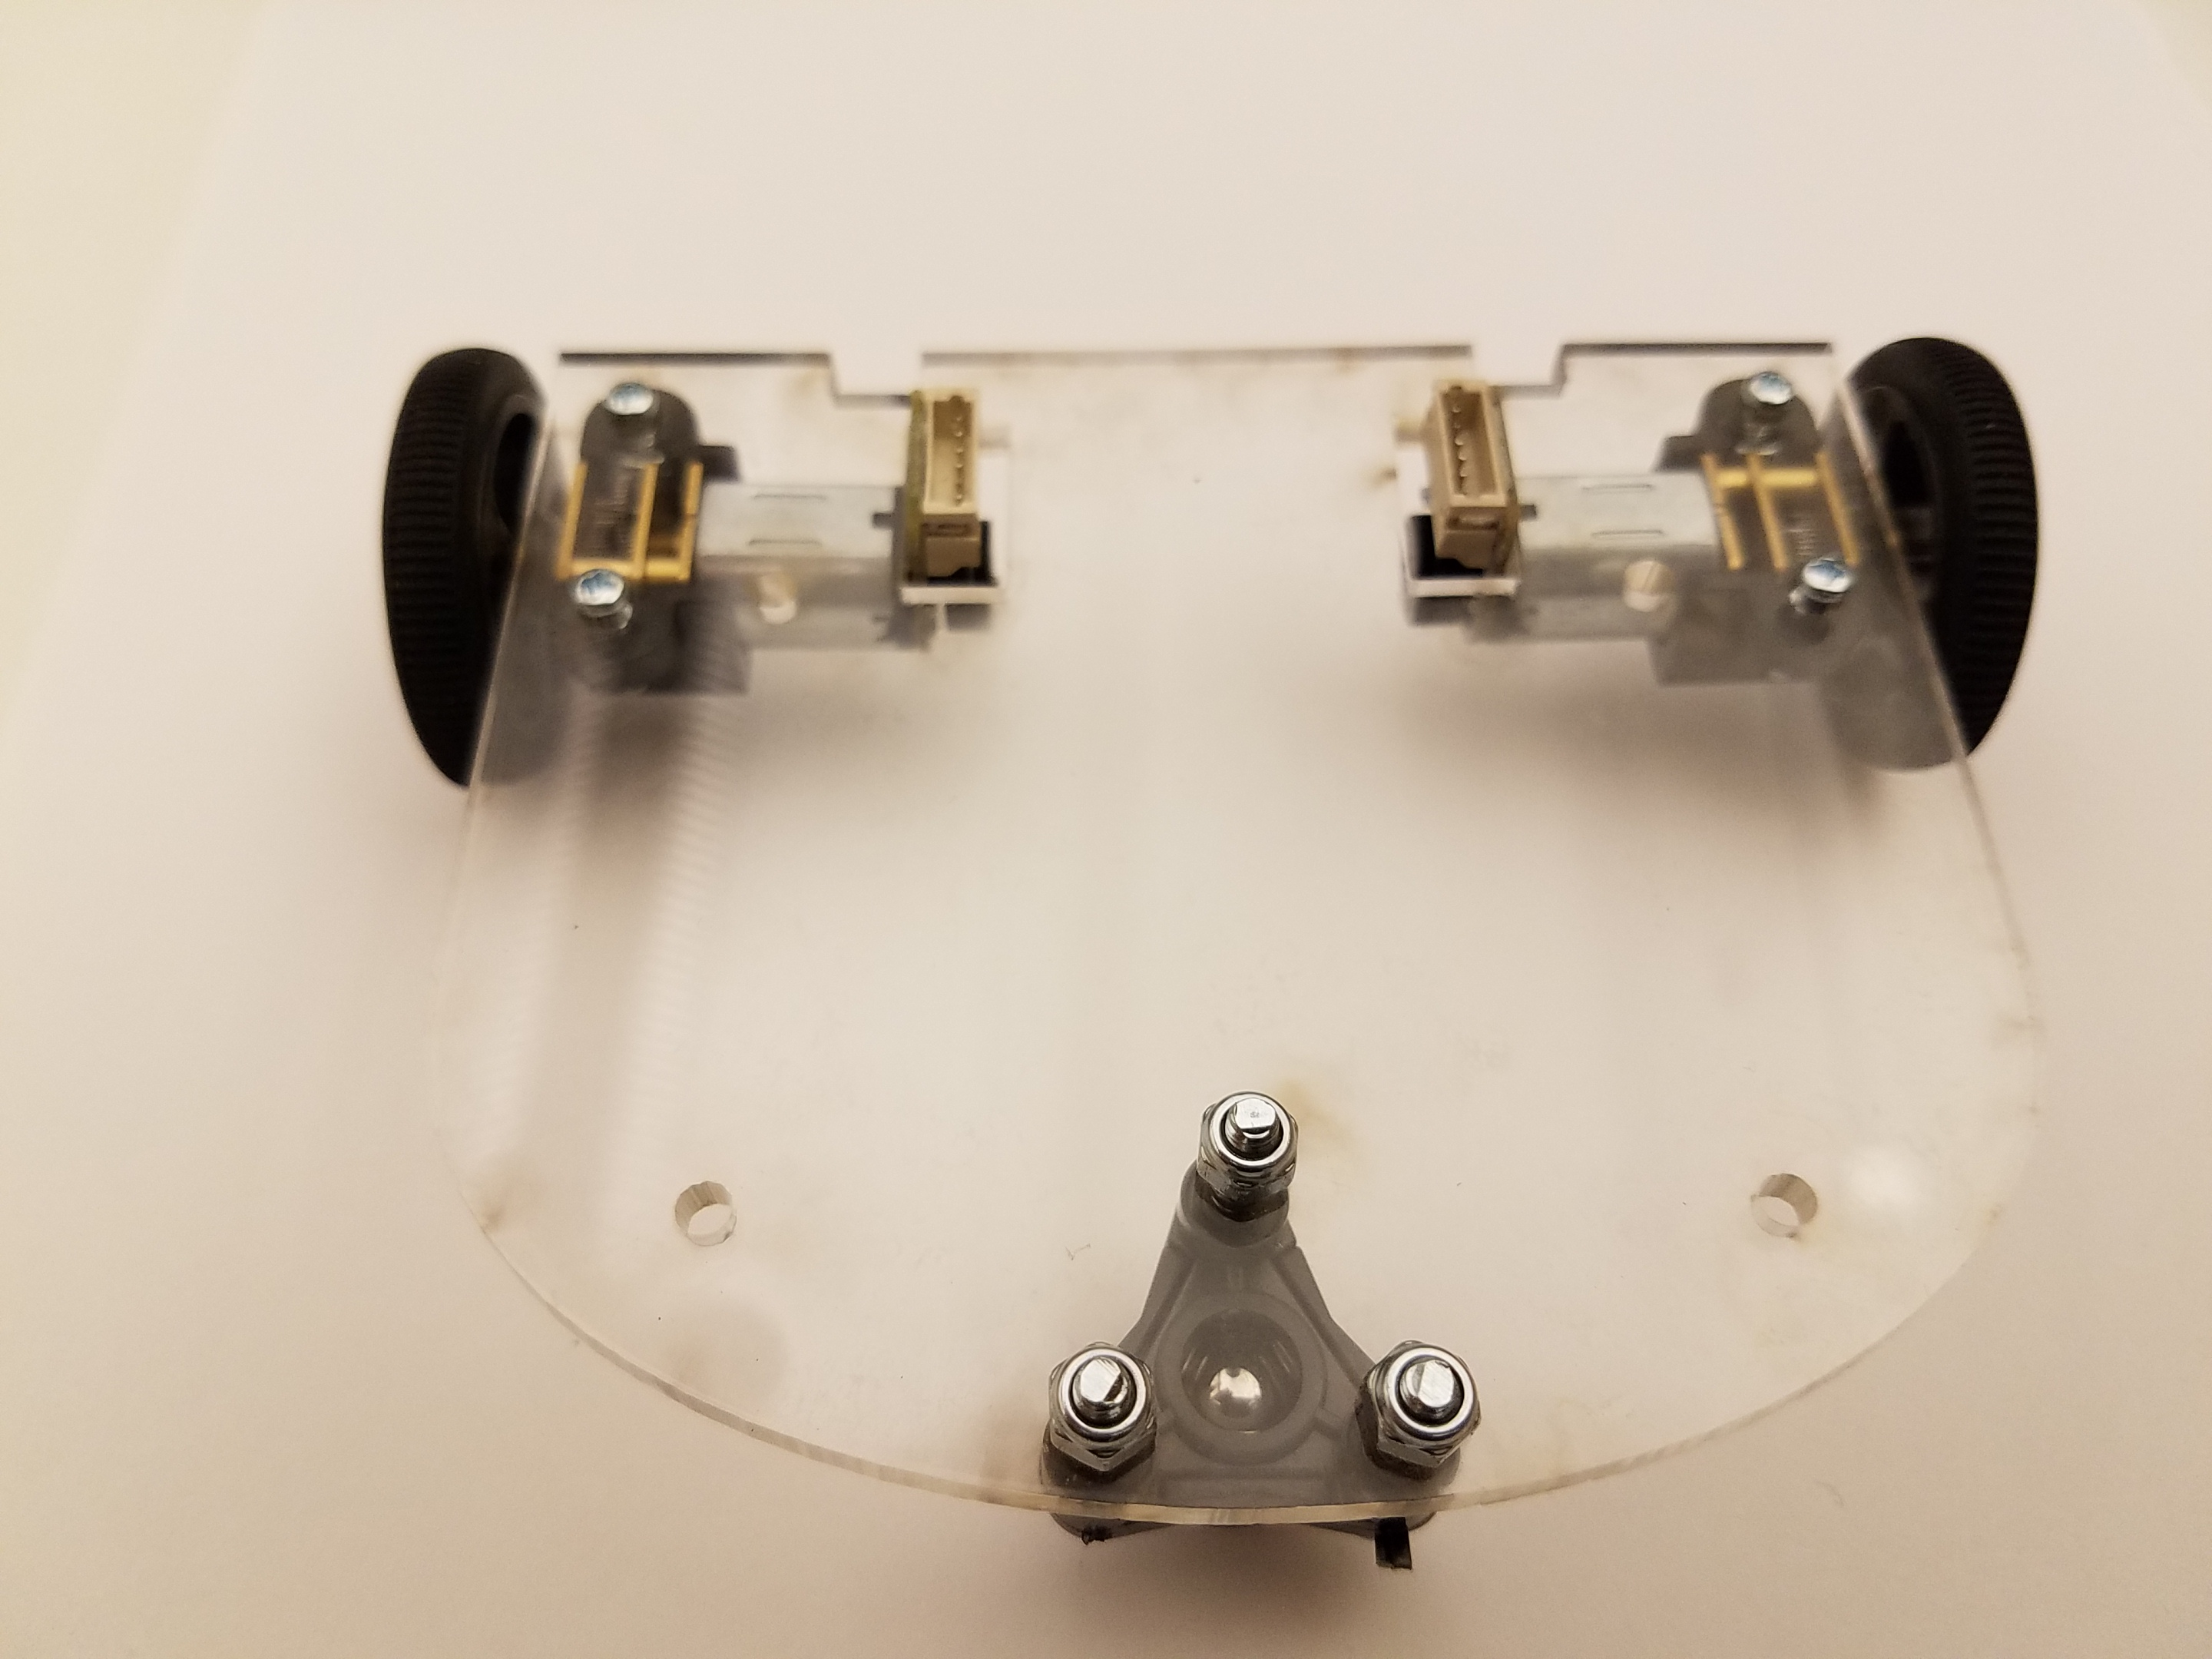
\includegraphics[width=0.65\columnwidth, keepaspectratio]{./figs/20181219_112632.jpg}
\caption{The chassis base of the GRITSBot X.}
\label{fig:finalBase}
\end{figure}
%End Finished Base Picture

\subsection{Putting Together the Battery Bracket}
\label{sec:BB}

\subsubsection{Assembly Steps}
\label{sec:BBSteps}

\begin{enumerate}
\item Gather the required materials (\cref{sec:BBParts}).
\item Snap together the acrylic battery box (\cref{sec:BBBox}).
\item Attach the spacers for mounting the battery box and PCB (\cref{sec:BBSpacers}).
\end{enumerate}

\subsubsection{Required Materials}
\label{sec:BBParts}

The battery box assembly is fairly straight forward. The battery box housing is a pressure fit box created by the four $1/16$ inch acrylic parts cut earlier and pictured in the top of \cref{fig:acrylic16}. The housing is then supported and attached to the robot by threaded hexagonal spacers. The full list of materials needed is shown in \cref{tab:BBParts}.

%Begin Battery Box Part Table
 \begin{table}[h!]
 \centering
\begin{tabular}{p{3in}c}
\rowcolor[HTML]{C0C0C0} 
\textbf{Part}  & \textbf{Number Required} 		\\
Acrylic Battery Bracket Top/Bottom		& 2	\\
\rowcolor[HTML]{C0C0C0} 
Acrylic Battery Bracket Side				& 2	\\
4-40, $5/16$ inch Female to Female Hexagonal Standoff	& 4	\\
\rowcolor[HTML]{C0C0C0} 
4-40, $5/16$ inch Male to Female Hexagonal Standoff	& 4  \\
4-40, $3/16$ inch Nylon Male to Female Hexagonal Standoff	& 4
\end{tabular}
\caption{The parts required to assemble the battery bracket of the GRITSBot X. \label{tab:BBParts}}
\end{table}
 %End Battery Box Part Table

\subsubsection{Snapping Together the Battery Box}
\label{sec:BBBox}

The battery box is assembled through pressure/press fitting tabs together to form a box. It should be noted this is a fairly delicate ($1/16$ inch acrylic is brittle and fragile) and precise process. If your laser cutter cuts wider or narrower paths than the one at Georgia Tech, the tab widths may have to be altered.

To begin, press fit two of the side pieces into a top/bottom piece as seen in \cref{fig:box1}. Note, if this seems to tight to do or the tabs don't hold together, the tab widths needs to be adjusted for your laser cutter. The best process to do this is to press in the center tab followed by the outside tabs. Try not to snap the acrylic during this.

%Battery Bracket Assembly Picture
\begin{figure}[h!]
\centering
\subfloat[\label{fig:box1} Battery bracket sides pressure fit into a top/bottom.]{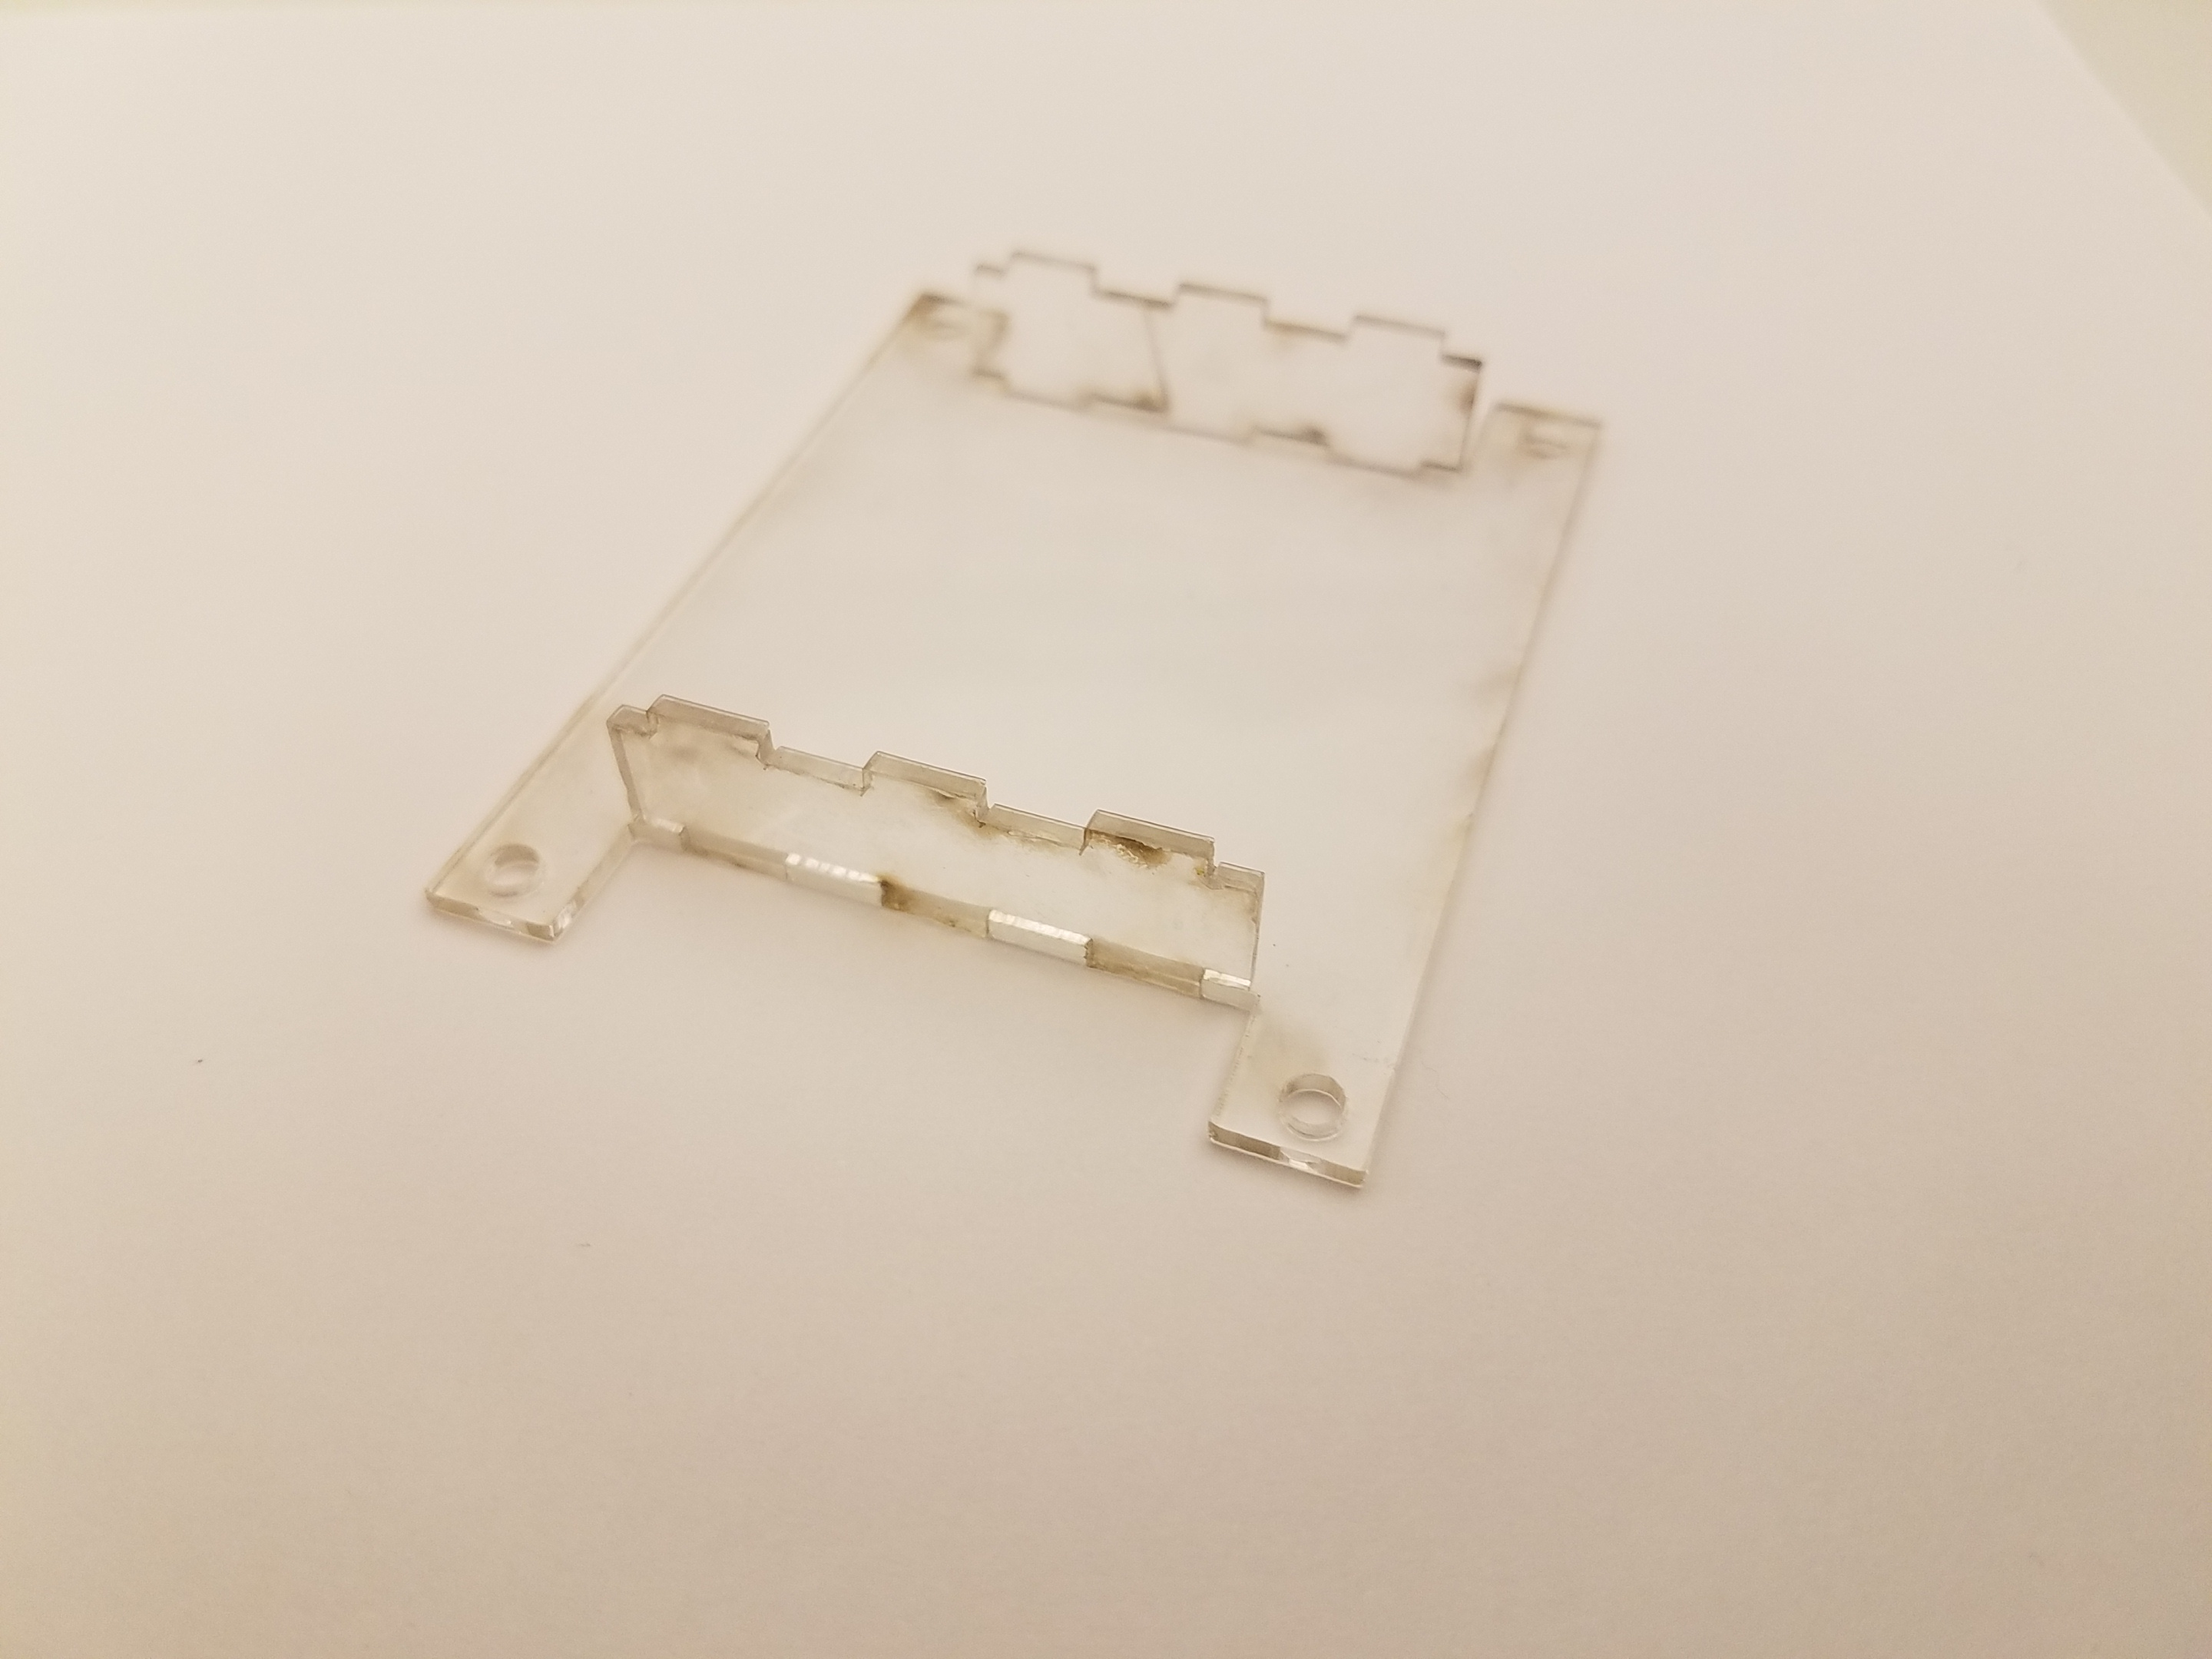
\includegraphics[width=0.45\columnwidth, keepaspectratio]{./figs/20181219_103937.jpg}}
\hfill
\subfloat[\label{fig:box2} Final battery bracket assembly.]{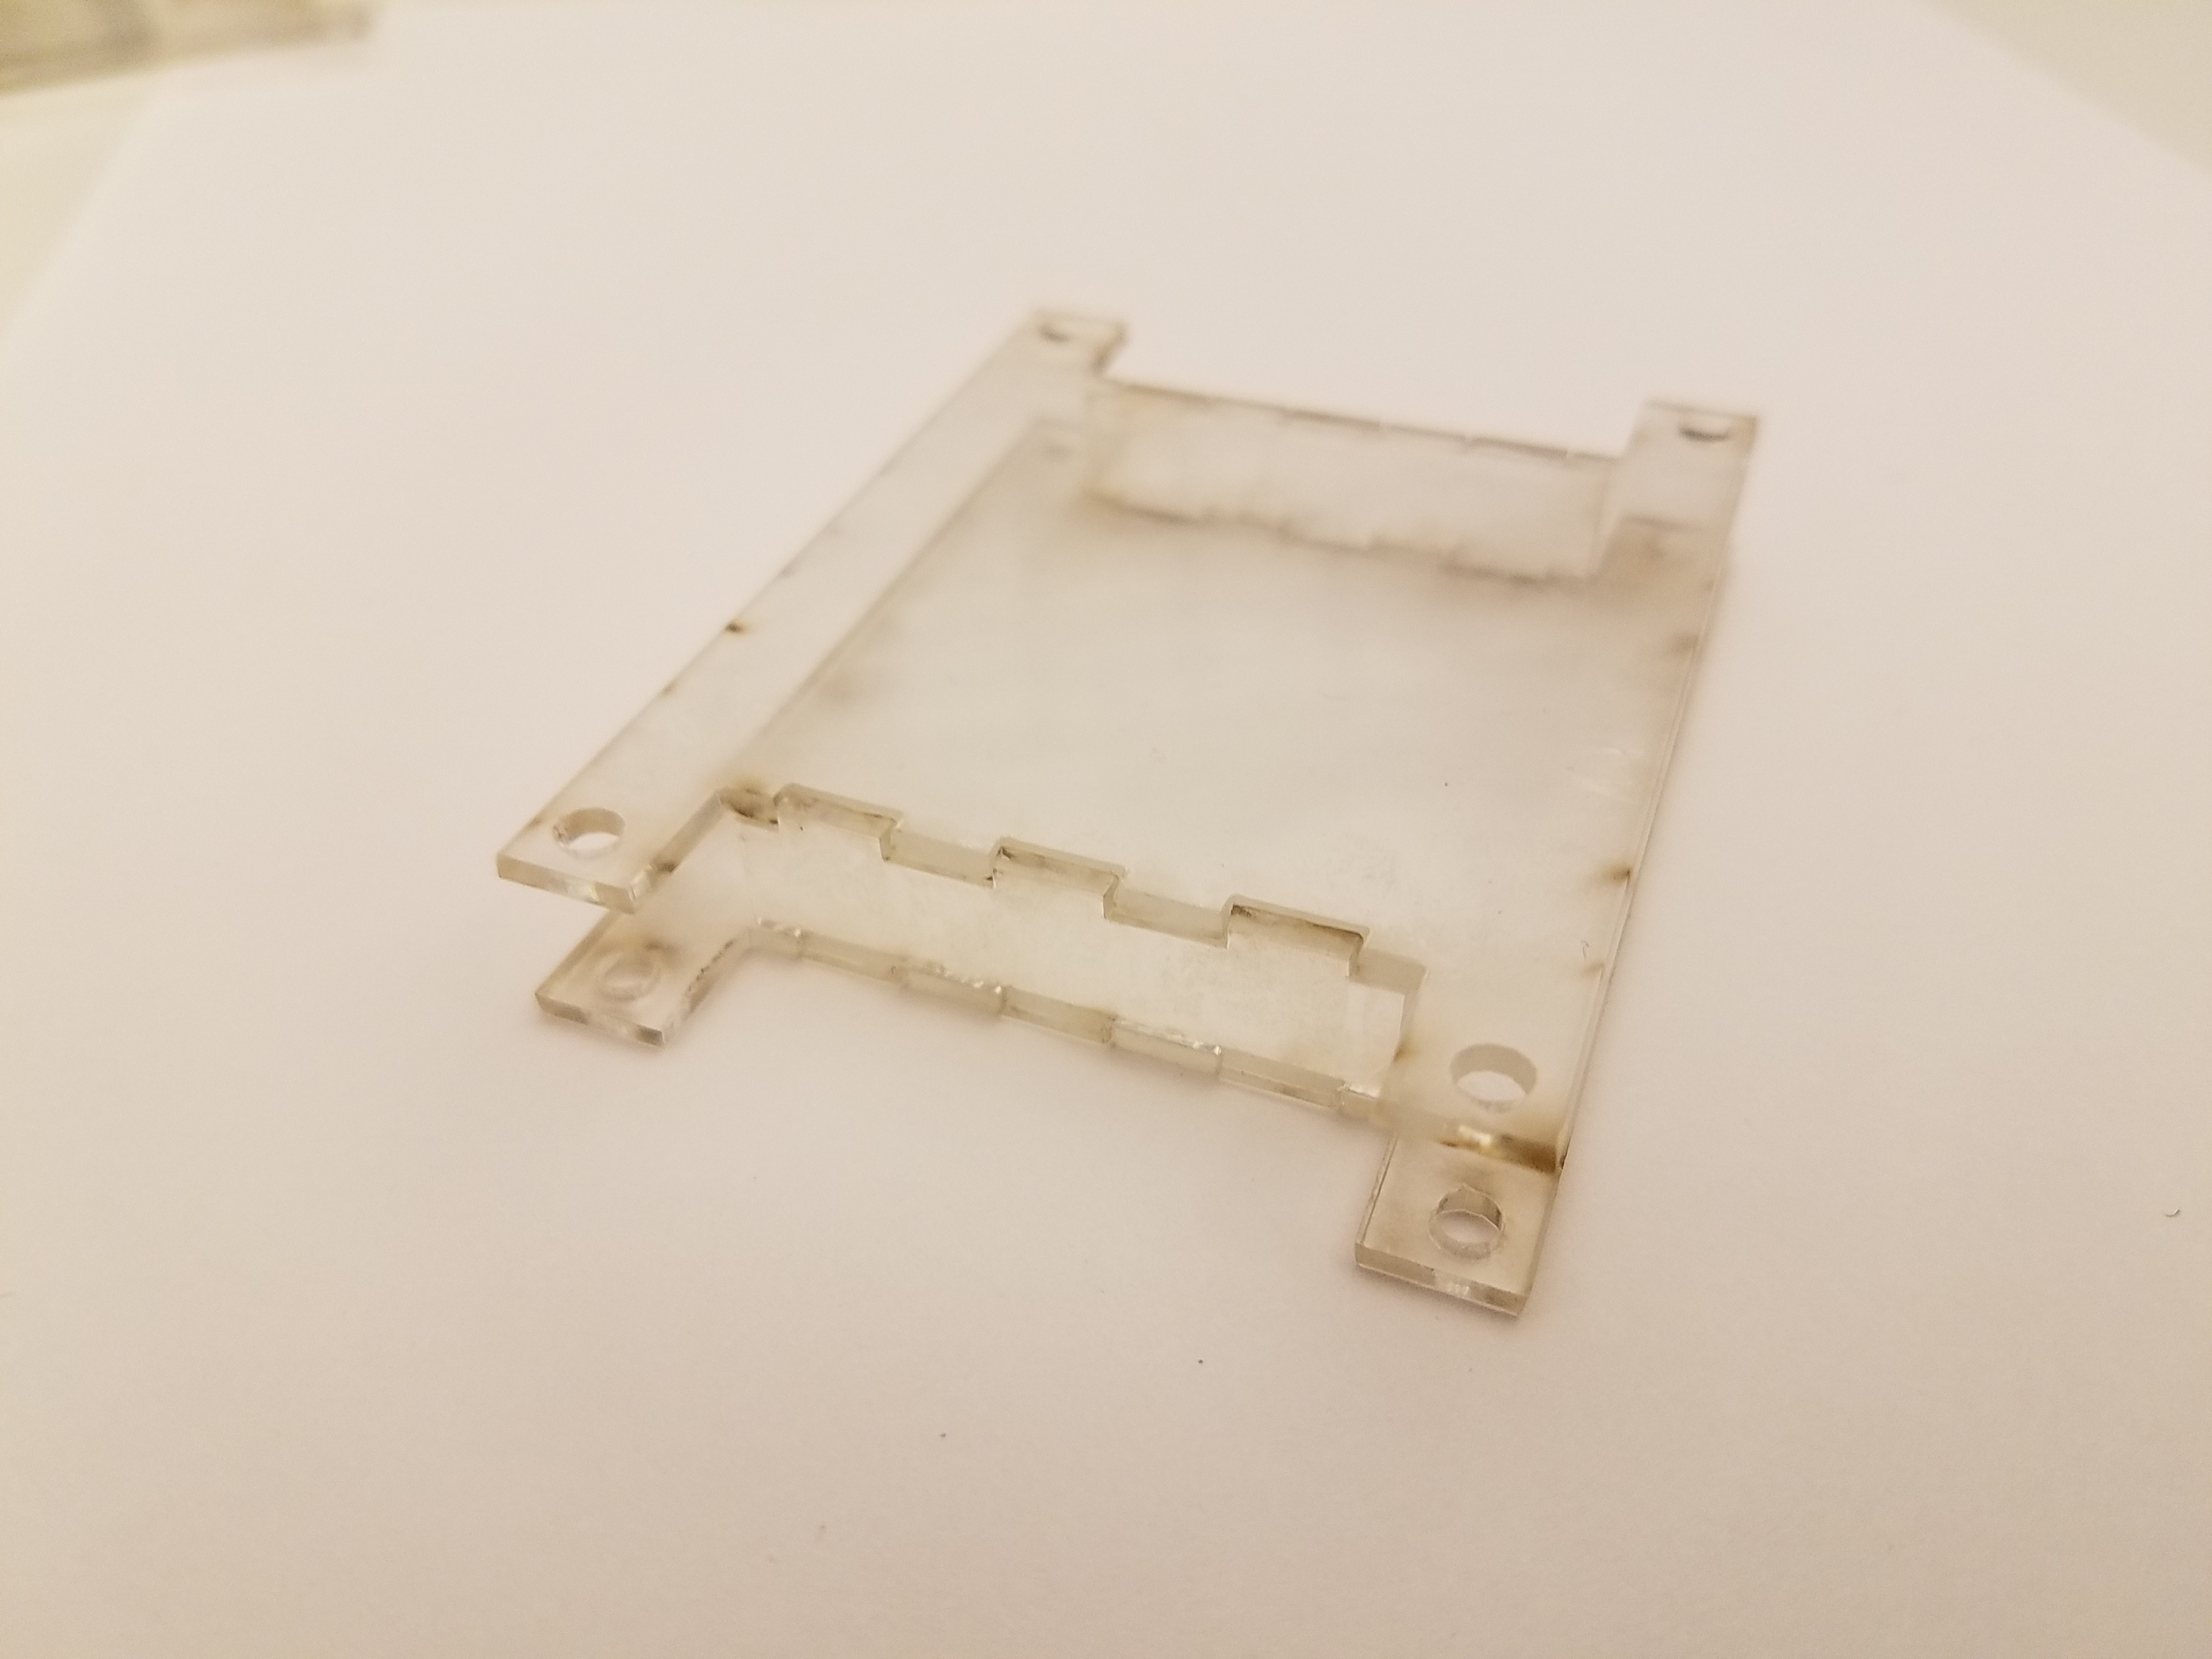
\includegraphics[width=0.45\columnwidth, keepaspectratio]{./figs/20181219_104108.jpg}}\\
\caption{Pressure/Press fitting together the battery bracket for the GRTISBot X.}
\label{fig:batteryBox}
\end{figure}
%End Battery Bracket Assembly Picture

Finally, press fit the top piece into the assembly just snapped together as seen in \cref{fig:box2}. It is much easier to press fit one side at a time. The joints should rotate fairly easily so you can press one at a time. pressing the assembly into the side of a table or book spine helps tremendously.

\subsubsection{Attaching the Mounting Spacers}
\label{sec:BBSpacers}

Finally, attach the hexagonal spacers to the battery box so it may be mounted to the base of the GRITSBot X and support the PCB in the next steps. Place the four $5/16$ female to female hexagonal spacers between the battery bracket (this can be done one at a time. Screw the four $5/16$ male to female hexagonal spacers into one side of the female to female spacers between the battery bracket. On the other side screw the four $3/16$ male to female nylon hexagonal spacers into the battery bracket. The resulting assembly should look like \cref{fig:finalBatteryBracket}.

 %Battery Bracket Finished Picture
\begin{figure}[h!]
\centering
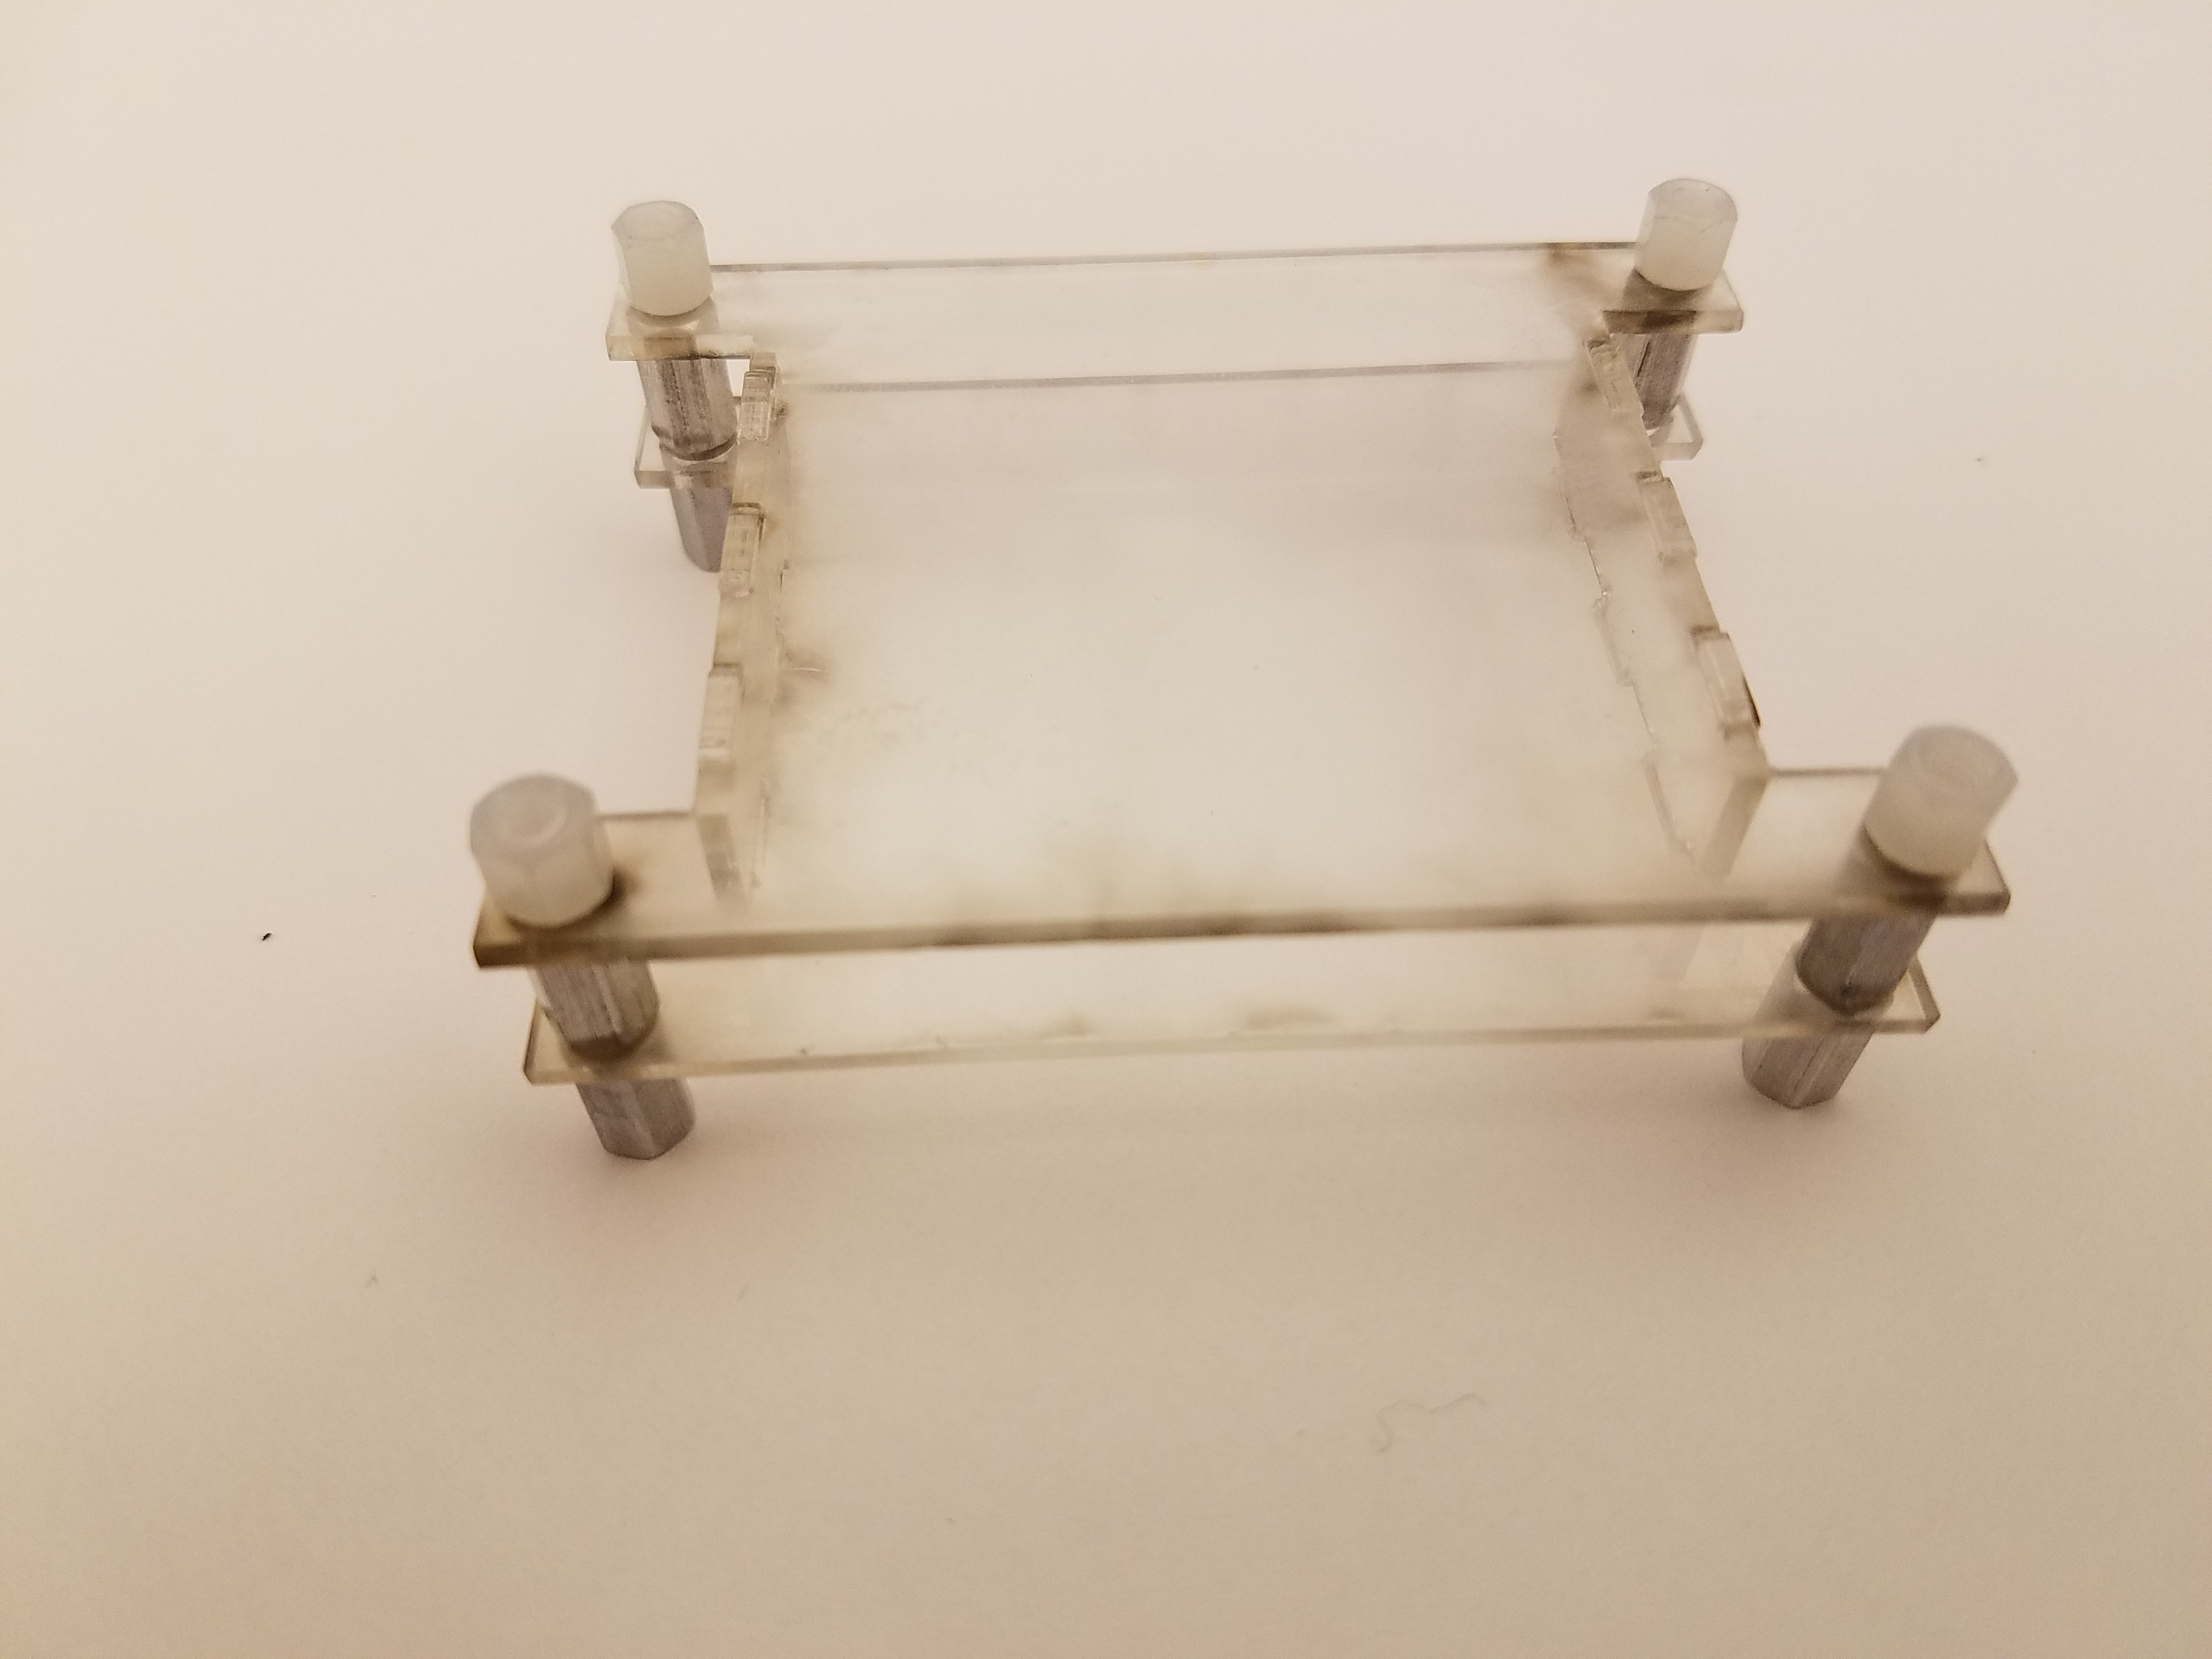
\includegraphics[width=0.65\columnwidth, keepaspectratio]{./figs/20190102_141824.jpg}
\caption{The finished battery bracket assembly with hexagonal stand off supports attached.}
\label{fig:finalBatteryBracket}
\end{figure}
%End Battery Bracket Finished Picture

\subsection{Attaching the Cassis Base, Battery Bracket, and PCB}
\label{sec:finishBase}

\subsubsection{Assembly Steps}
\label{sec:finishBaseSteps}

\begin{enumerate}
\item Gather the required materials (\cref{sec:finishBaseMaterials}).
\item Attach the battery box to the chassis base (\cref{sec:BBtoCB}).
\item Attach the PCB to the chassis base assembly (\cref{sec:attachPCB}).
\end{enumerate}

\subsubsection{Required Materials}
\label{sec:finishBaseMaterials}

Connecting the chassis base, battery bracket, and PCB is, again, straightforward and just requires screwing the parts created previously together. The full list of materials needed are in \cref{tab:finishBaseParts}.

%Begin Chassis Base Part Table
 \begin{table}[h!]
 \centering
\begin{tabular}{p{3in}c}
\rowcolor[HTML]{C0C0C0} 
\textbf{Part}  & \textbf{Number Required} 		\\
Assembled Chassis Base from \cref{sec:base}		& 1	\\
\rowcolor[HTML]{C0C0C0} 
Assembled Battery Bracket from \cref{sec:BB}				& 1	\\
Finished PCB from \cref{sec:pcb}	& 1	\\
\rowcolor[HTML]{C0C0C0} 
4-40, $1/4$ inch Screw	& 4  \\
4-40, $3/4$ inch Nylon Male to Female Hexagonal Standoff	& 4\\
\rowcolor[HTML]{C0C0C0} 
3.7V 2500mAh Adafruit Li-Po Battery	& 1
\end{tabular}
\caption{The parts required to combine the chassis base, battery bracket, and PCB of the GRITSBot X. \label{tab:finishBaseParts}}
\end{table}
 %End Chassis Base Part Table


\subsubsection{Attaching the Battery Box to the Chassis Base}
\label{sec:BBtoCB}

The battery bracket assembly (\cref{fig:finalBatteryBracket}, assembly instructions in \cref{sec:BB}) attaches directly to the chassis base (\cref{fig:finalBase}, assembly instructions in \cref{sec:base}) Screw the four 4-40, $1/4$ inch screws,  through the bottom of the four remaining holes in the acrylic base plate into the four 4-40, $5/16$ inch hexagonal standoffs. If done properly, the battery bracket, chassis base assembly should look like \cref{fig:BBtoBC}.

 %Battery Bracket Chassis Finished Picture
\begin{figure}[h!]
\centering
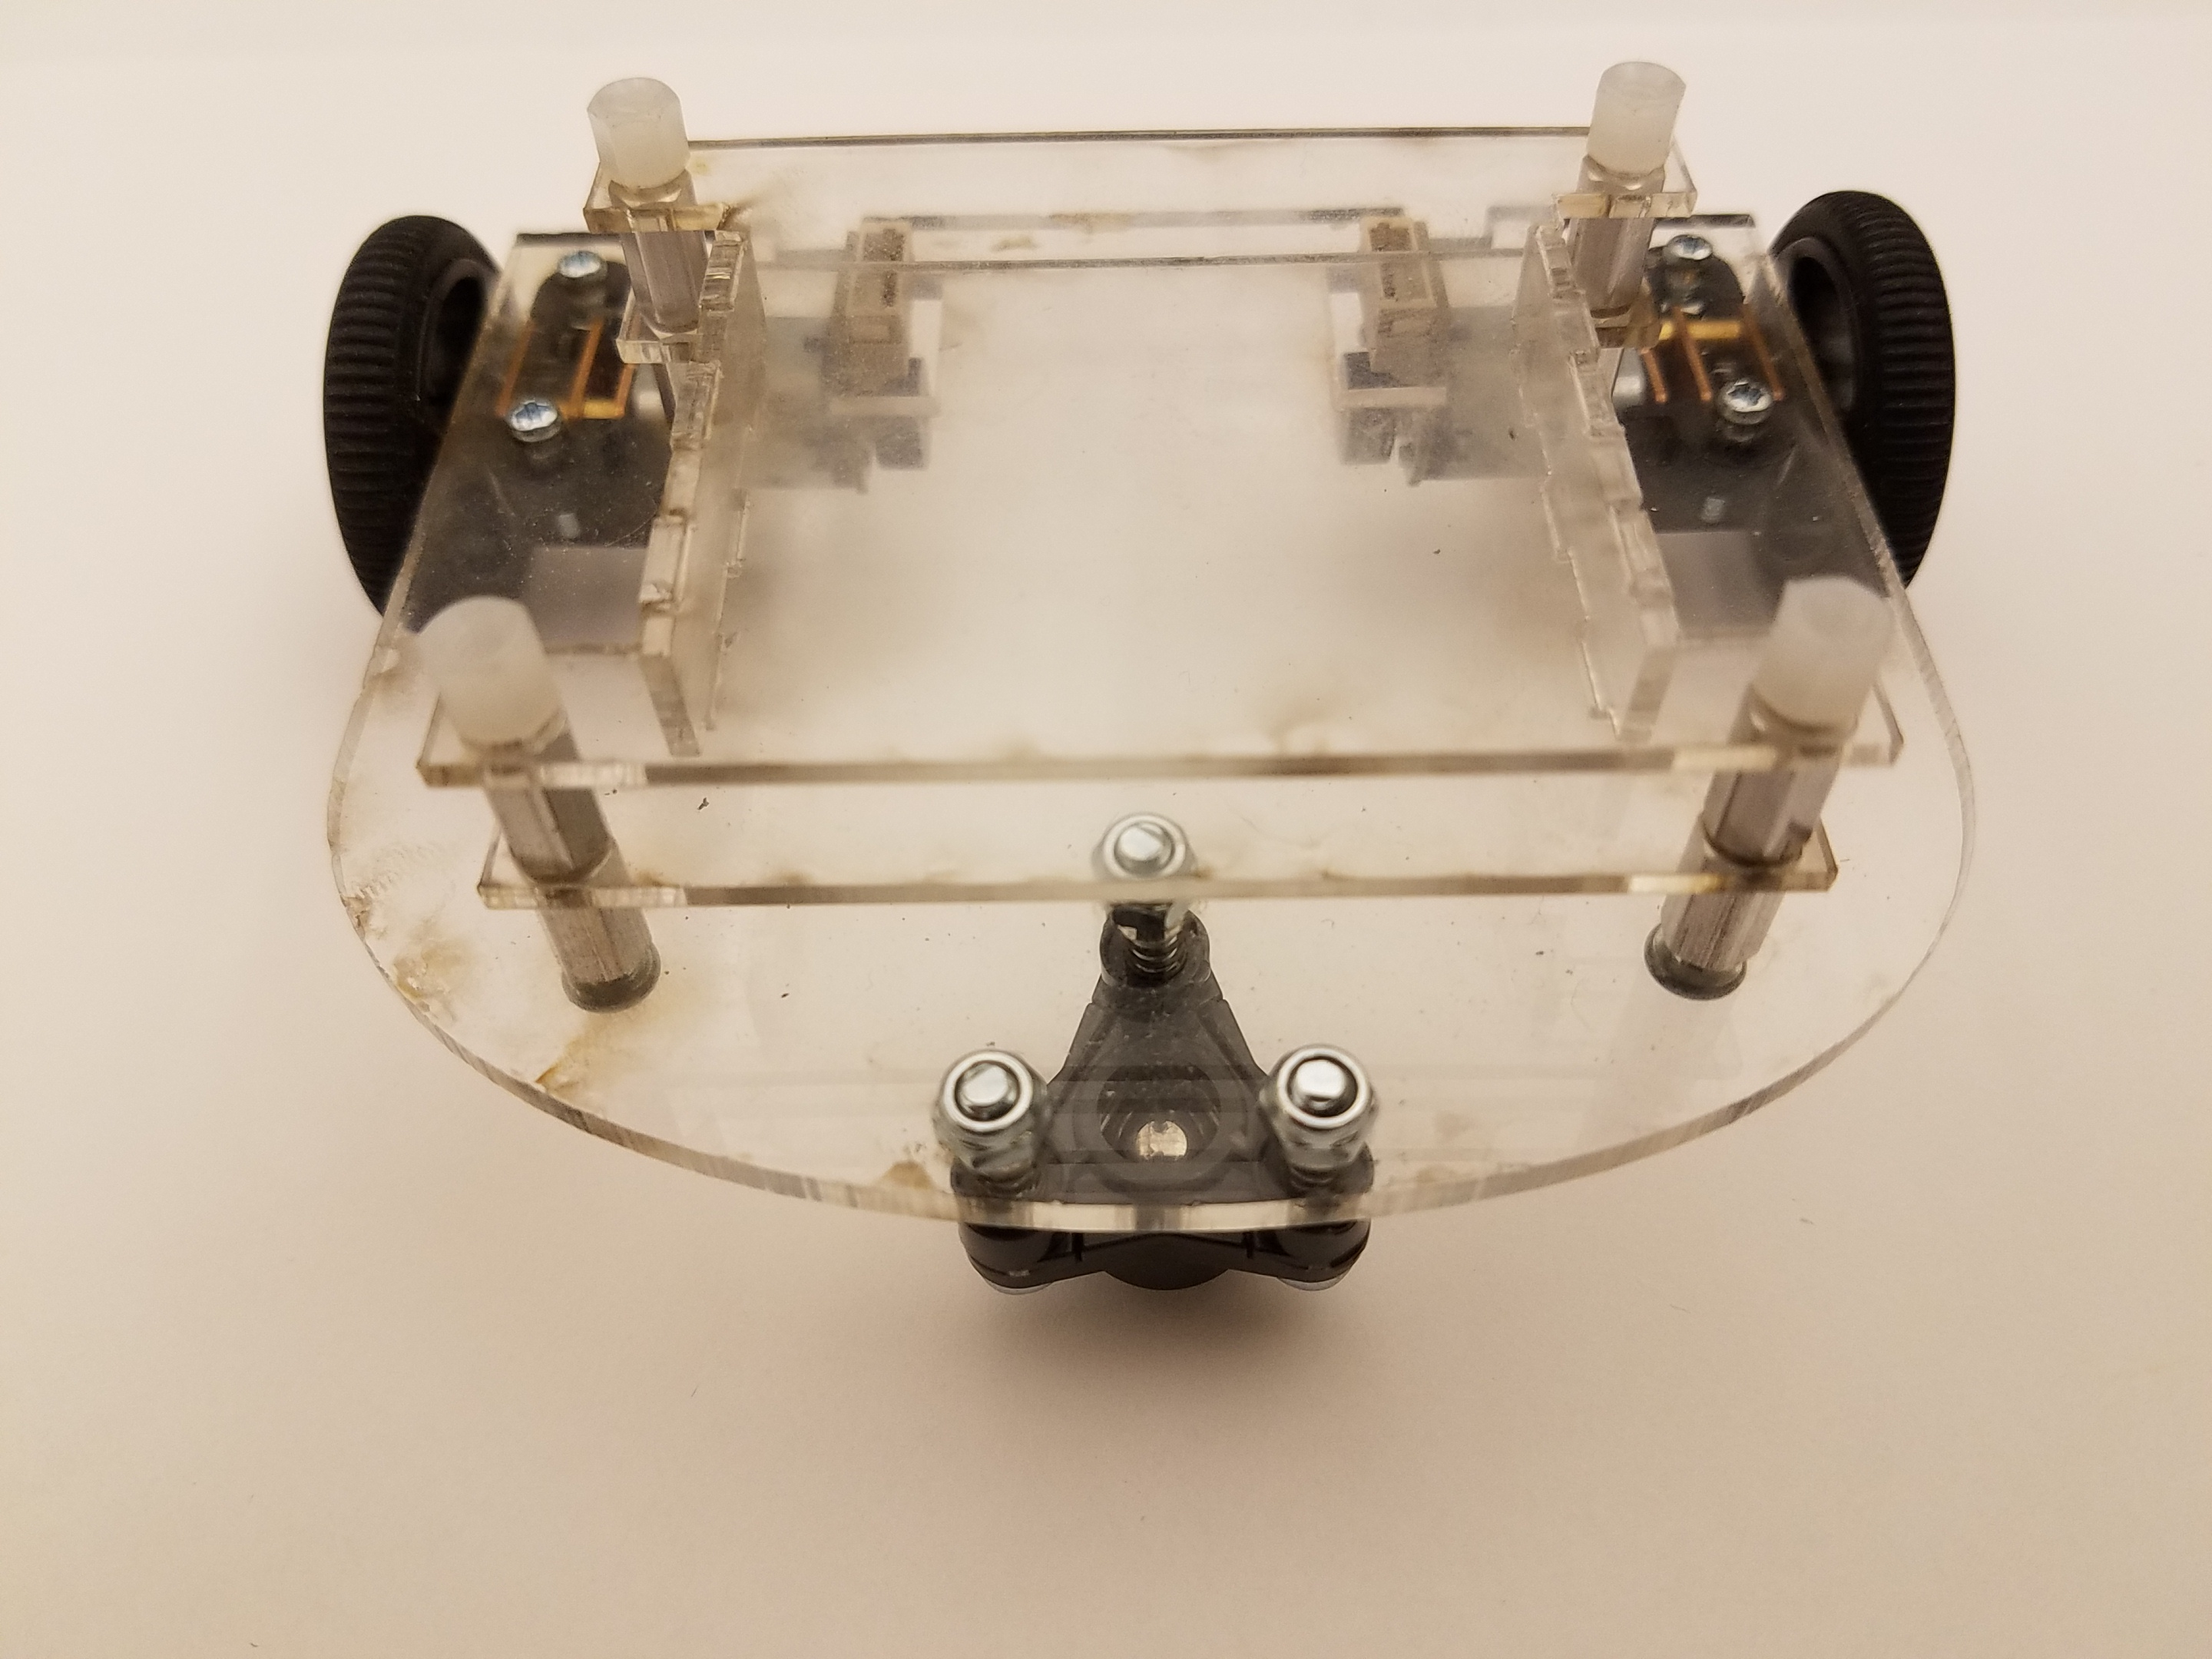
\includegraphics[width=0.65\columnwidth, keepaspectratio]{./figs/20190103_140414.jpg}
\caption{The base chassis with batter bracket attached.}
\label{fig:BBtoBC}
\end{figure}
%End Battery Bracket Chassis Finished Picture

\subsubsection{Attaching the PCB}
\label{sec:attachPCB}

Attaching the PCB is a little trickier simply because the motor leads danging from the PCB must be attached to the motor and the battery lead must be run in a somewhat smart way. The PCB aligns with the chassis shape, the round part of the board should line up with the round part of the chassis when attached. The top of the PCB has the Teensy micro-controller on it. After orienting it correctly, the four holes on the board should line up with the four 4-40, $3/16$ inch nylon hexagonal stand offs. Before securing the PCB into place, run the motor leads around the side of the battery box, underneath it, along the base acrylic, and out between the motor connections. The left lead from the PCB should insert into the left motor and right lead from the PCB should insert into the right motor. {\color{red}{Note}}, there is a tab on the connection so it should only insert one way but can be forced in the wrong way which will break the robot if powered on this way!

To clean up the excess wire push it back underneath the battery bracket such that there is enough room to insert the 3.7V Li-Po battery into the battery box. Insert the battery such that the lead comes out the back (flat side of the chassis) of the robot. Run the lead under the battery bracket (above the base acrylic) and out the left side of the robot to the battery connector (black plastic connector towards the back left corner of the PCB). {\color{red}{Note}}, make sure the lead of the battery is bent away from the wheel so it does not get caught and stall the robot or wear away the insulation. The wiring should look like \cref{backAttachPCB} when finished.

If done correctly the robot with the PCB in place should look like \cref{fig:attachPCB}.

%Battery Bracket Assembly Picture
\begin{figure}[h!]
\centering
\subfloat[\label{fig:topAttachPCB} Top view of the GRITSBot X with PCB attached to the chassis base.]{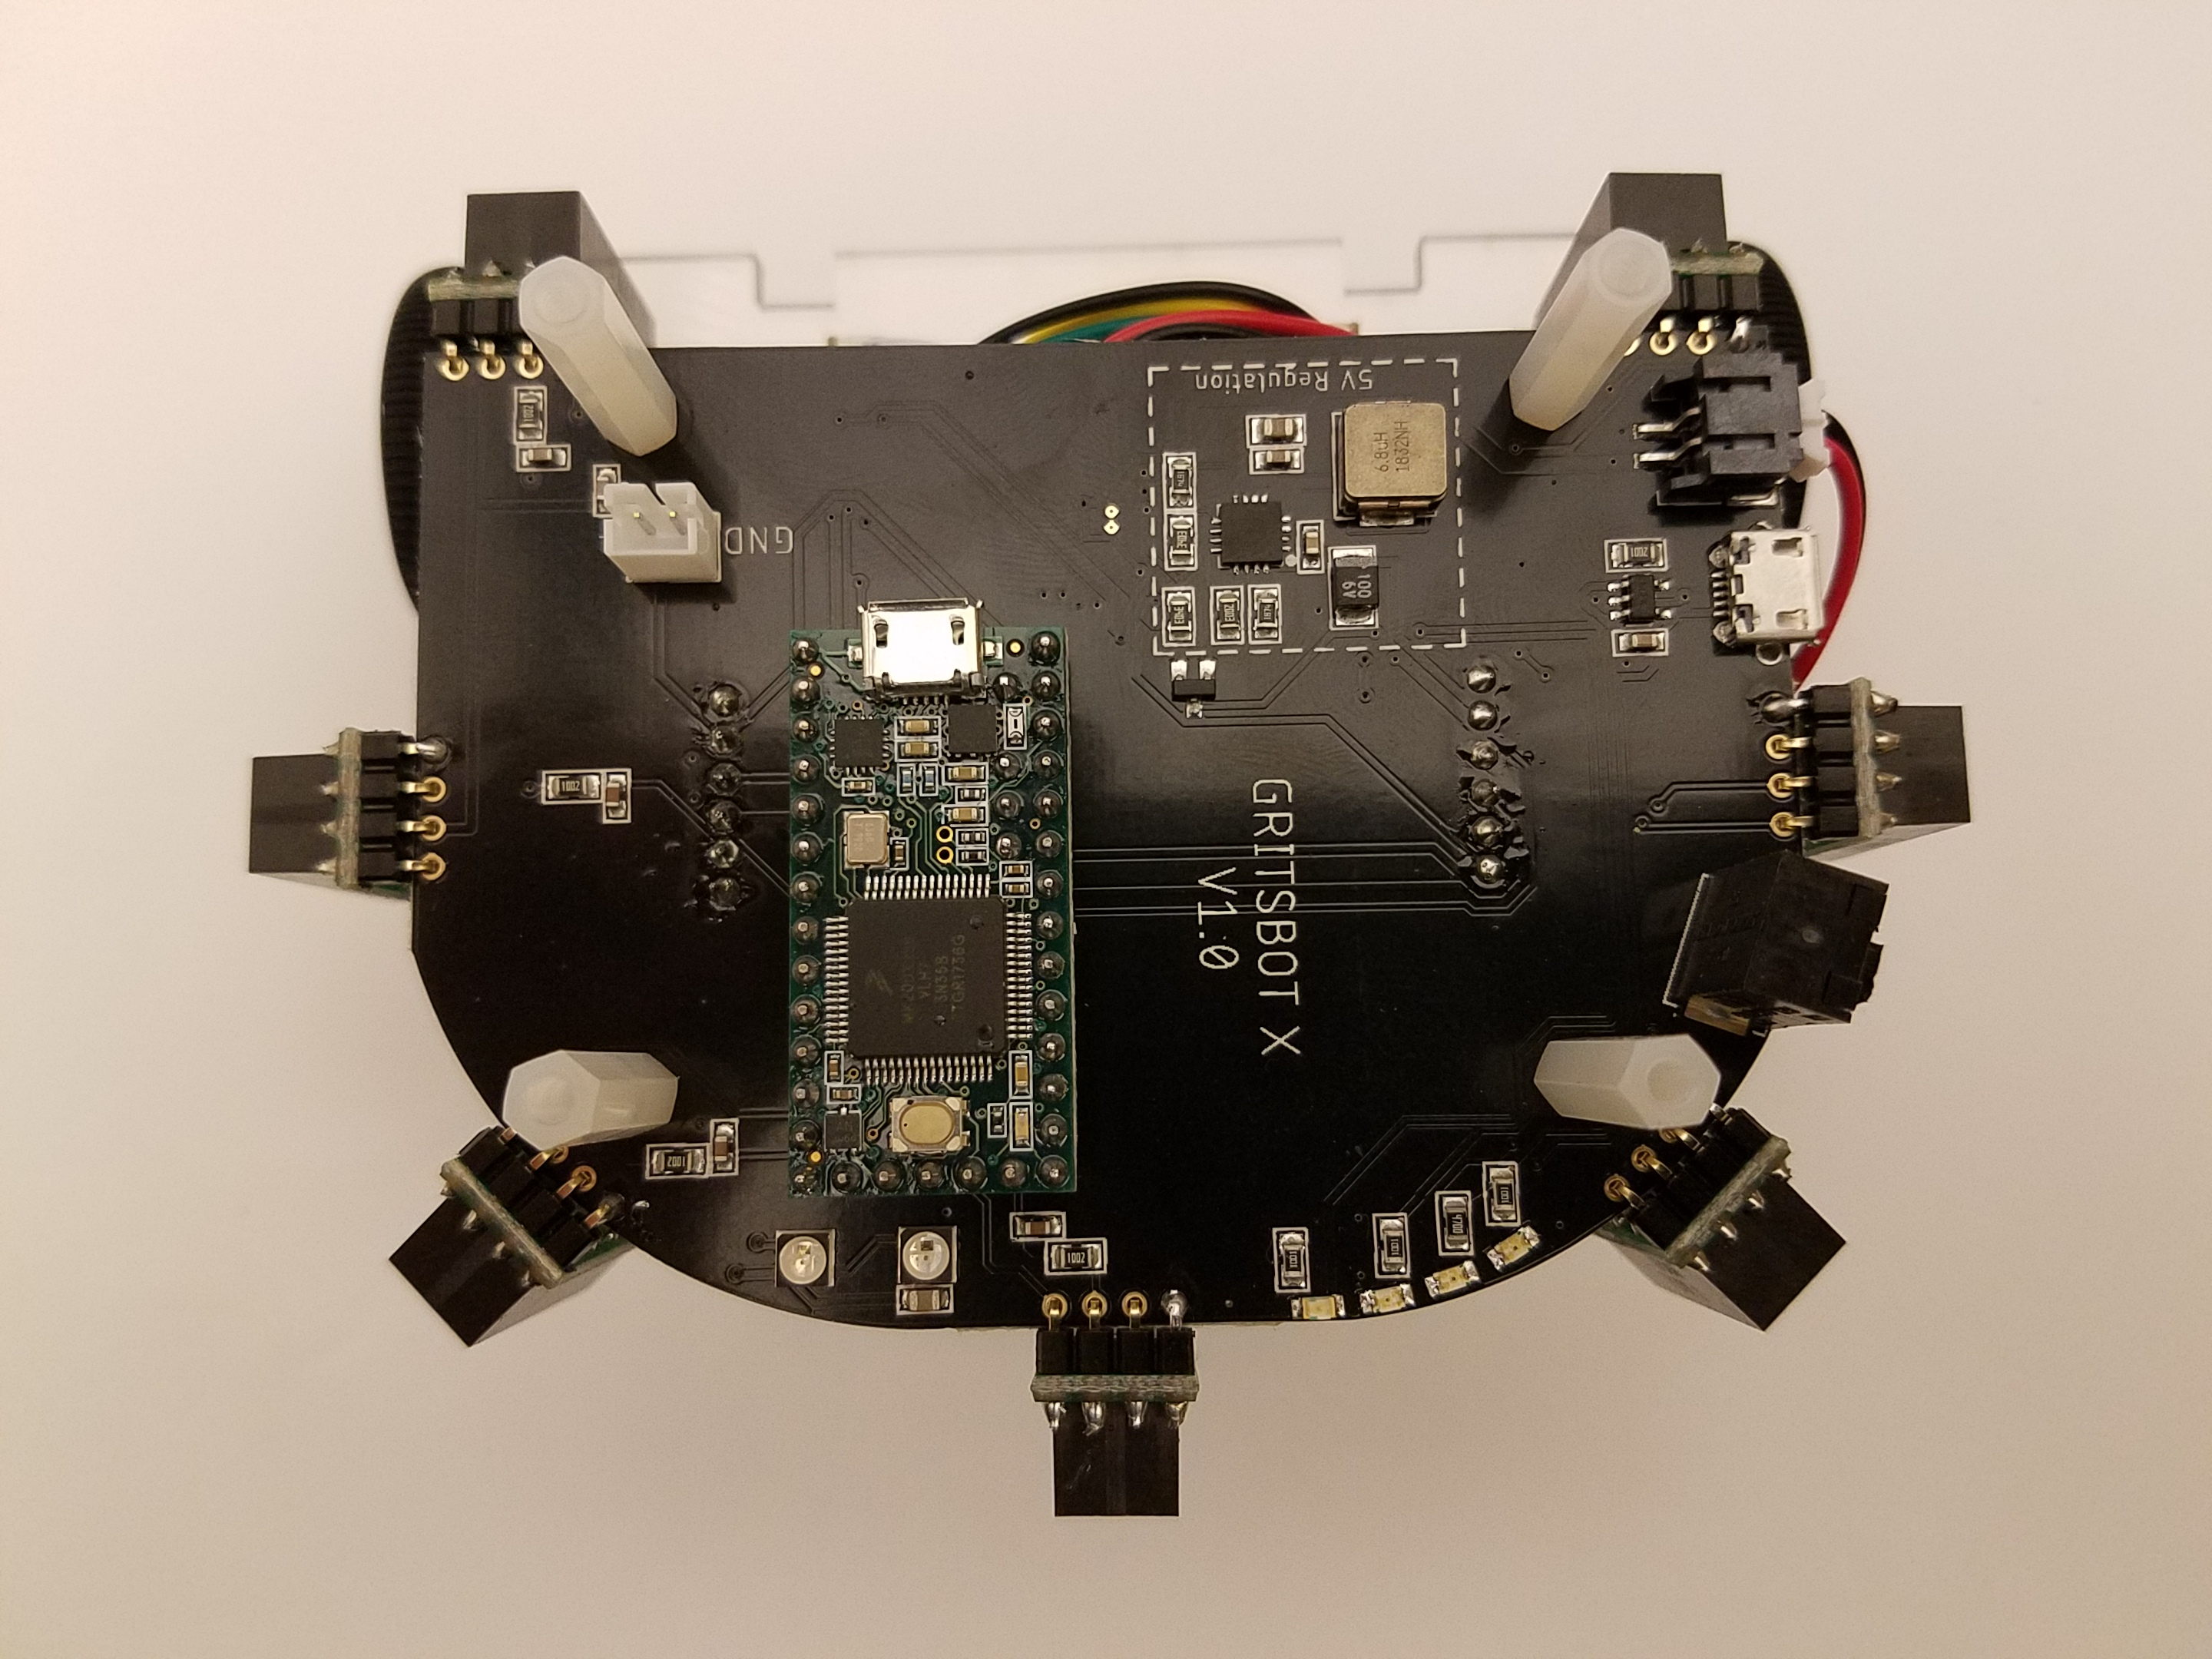
\includegraphics[width=0.45\columnwidth, keepaspectratio]{./figs/20190103_133104.jpg}}
\hfill
\subfloat[\label{fig:backAttachPCB} Back view of the GRITSBot X with PCB attached to the chassis base.]{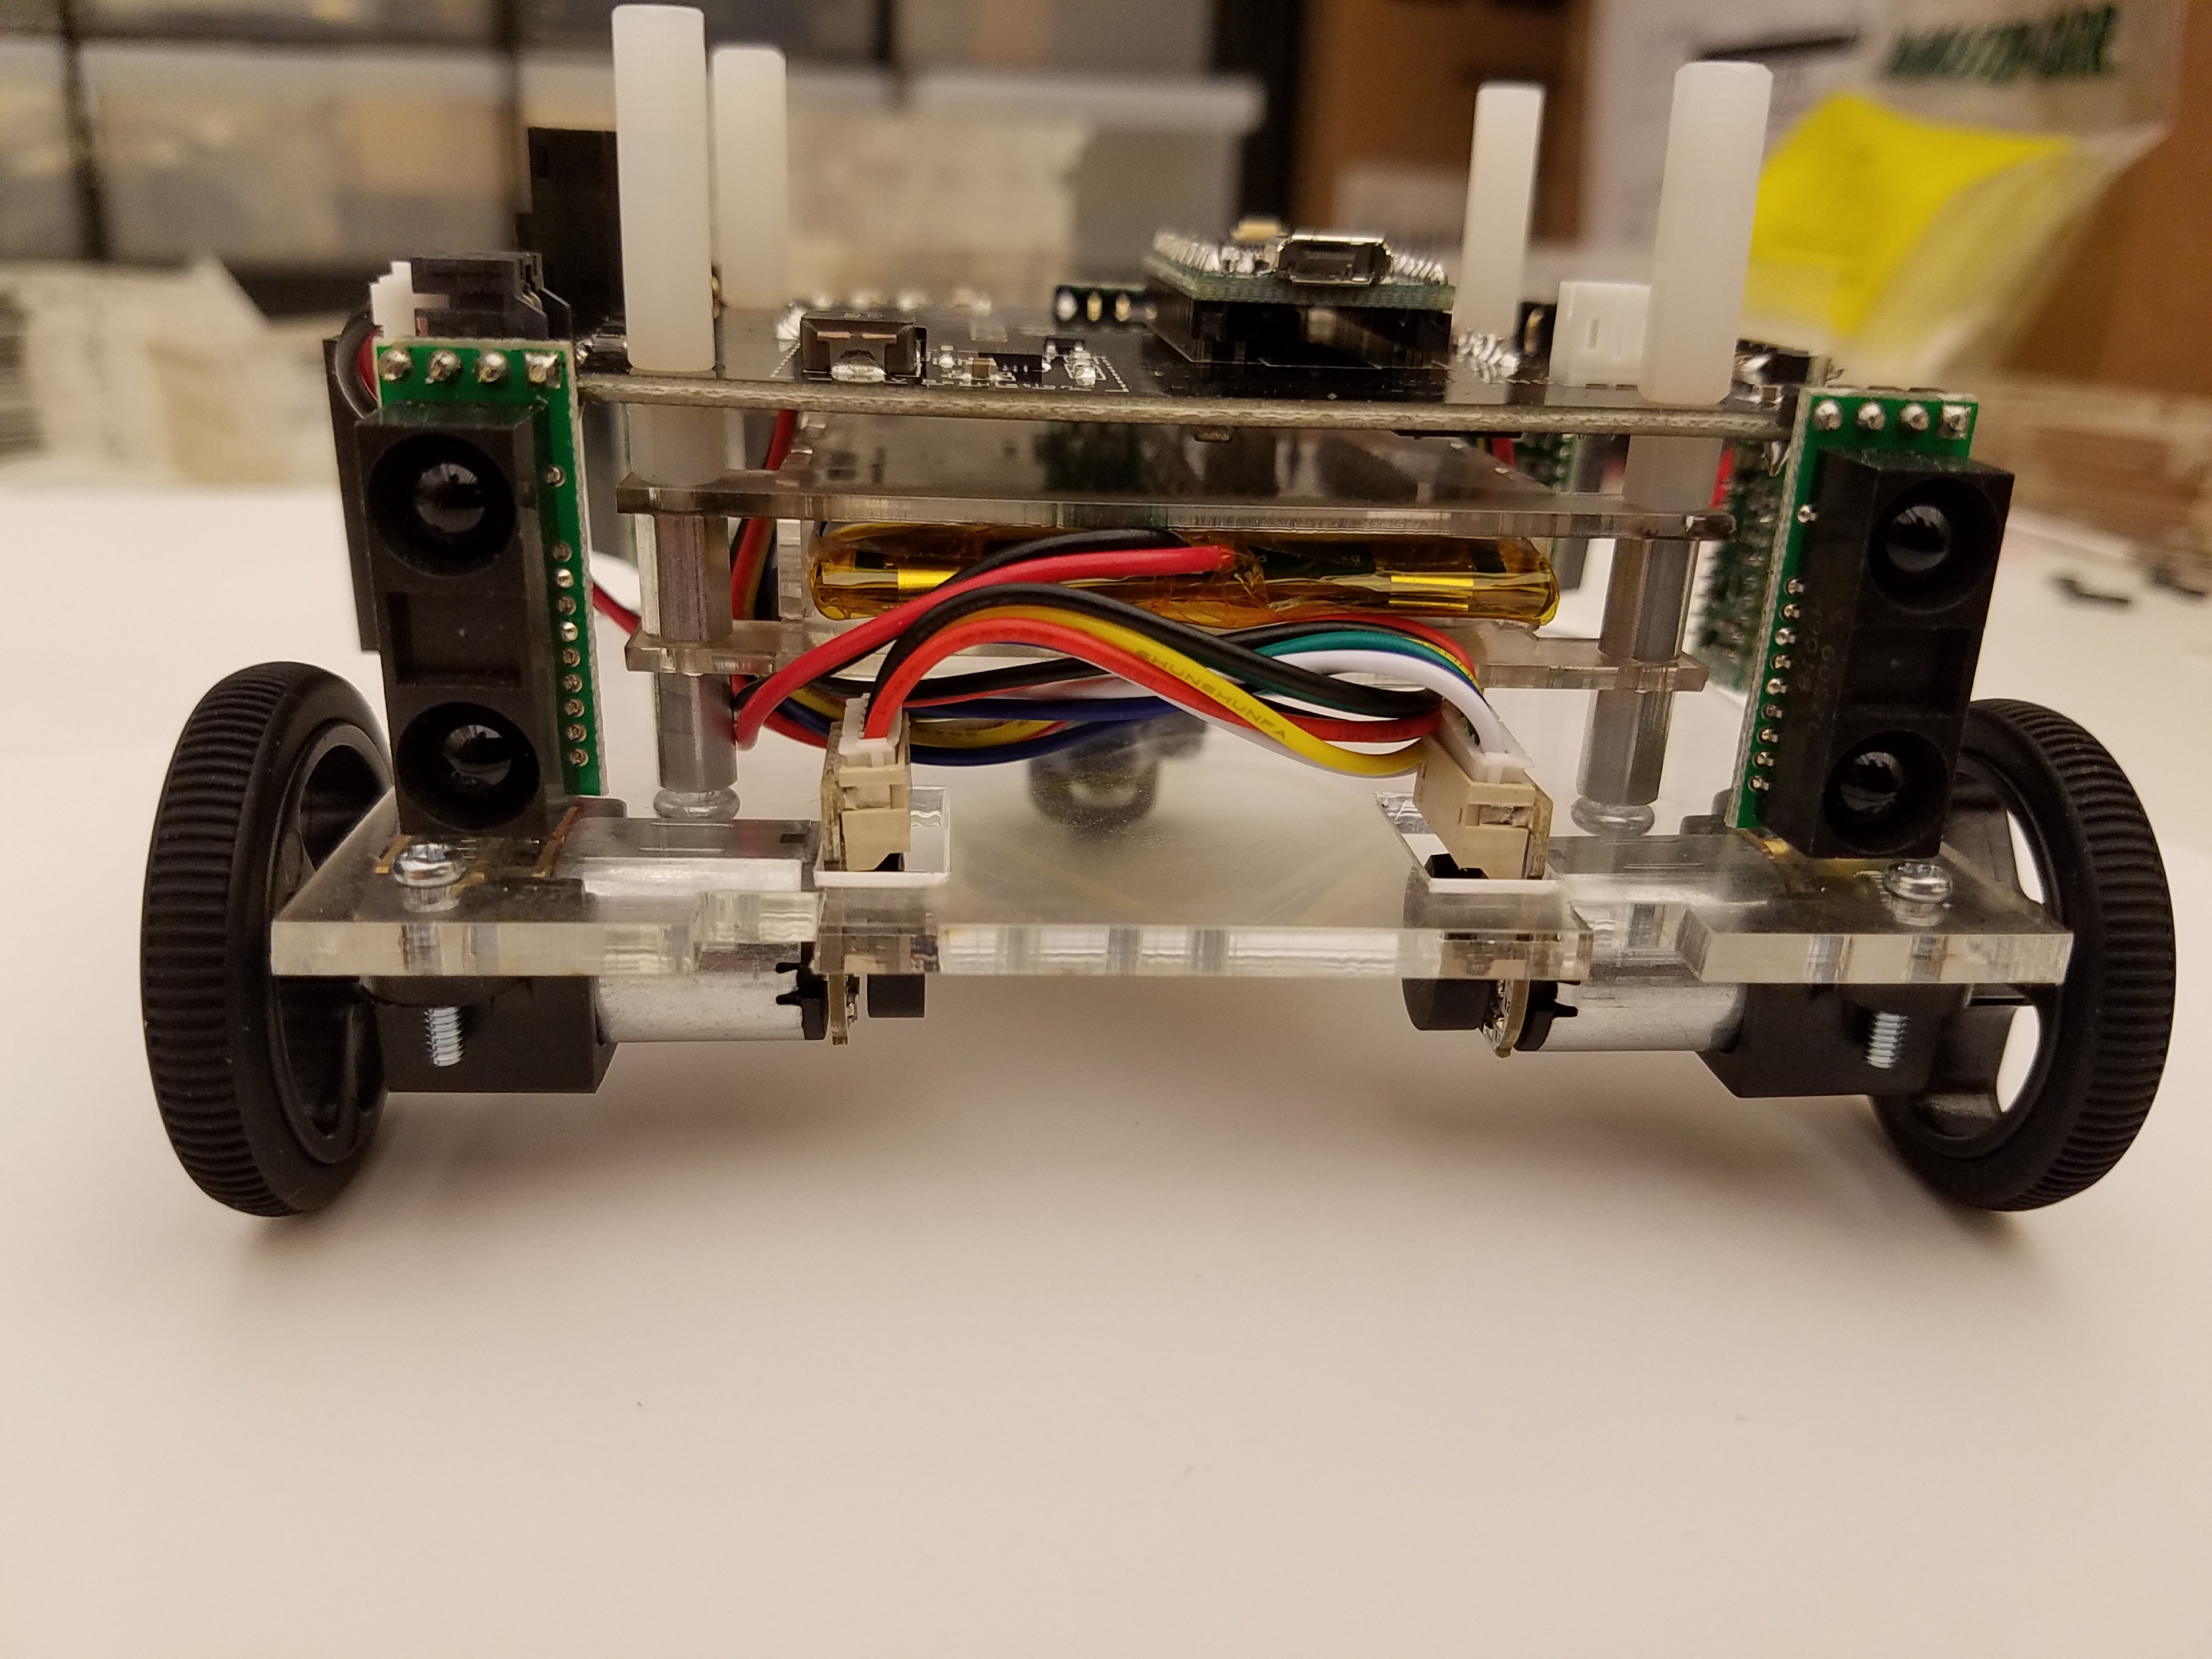
\includegraphics[width=0.45\columnwidth, keepaspectratio]{./figs/20190103_133137.jpg}}\\
\caption{The GRITSBot X without top assembly.}
\label{fig:attachPCB}
\end{figure}
%End Battery Bracket Assembly Picture

\subsection{Assembling and Attaching the Chassis Cover}
\label{sec:topPlate}

\subsubsection{Assembly Steps}
\label{sec:topPlateSteps}

\begin{enumerate}
\item Gather the required materials (\cref{sec:topPlateMaterials}).
\item Attach the Raspberry Pi to the Zero4U through the top acrylic plate (\cref{sec:attachZero4U}).
\item Attach the chassis top assembly to the base assembly (\cref{sec:attachChassisTop}).
\end{enumerate}

\subsubsection{Required Materials}
\label{sec:topPlateMaterials}

The chassis is nearly assembled and thus, there are not many materials needed for this step. The few needed are  listed in \cref{tab:topPlateMaterials}.

%Top Chassis Materials Picture
\begin{figure}[h!]
\centering
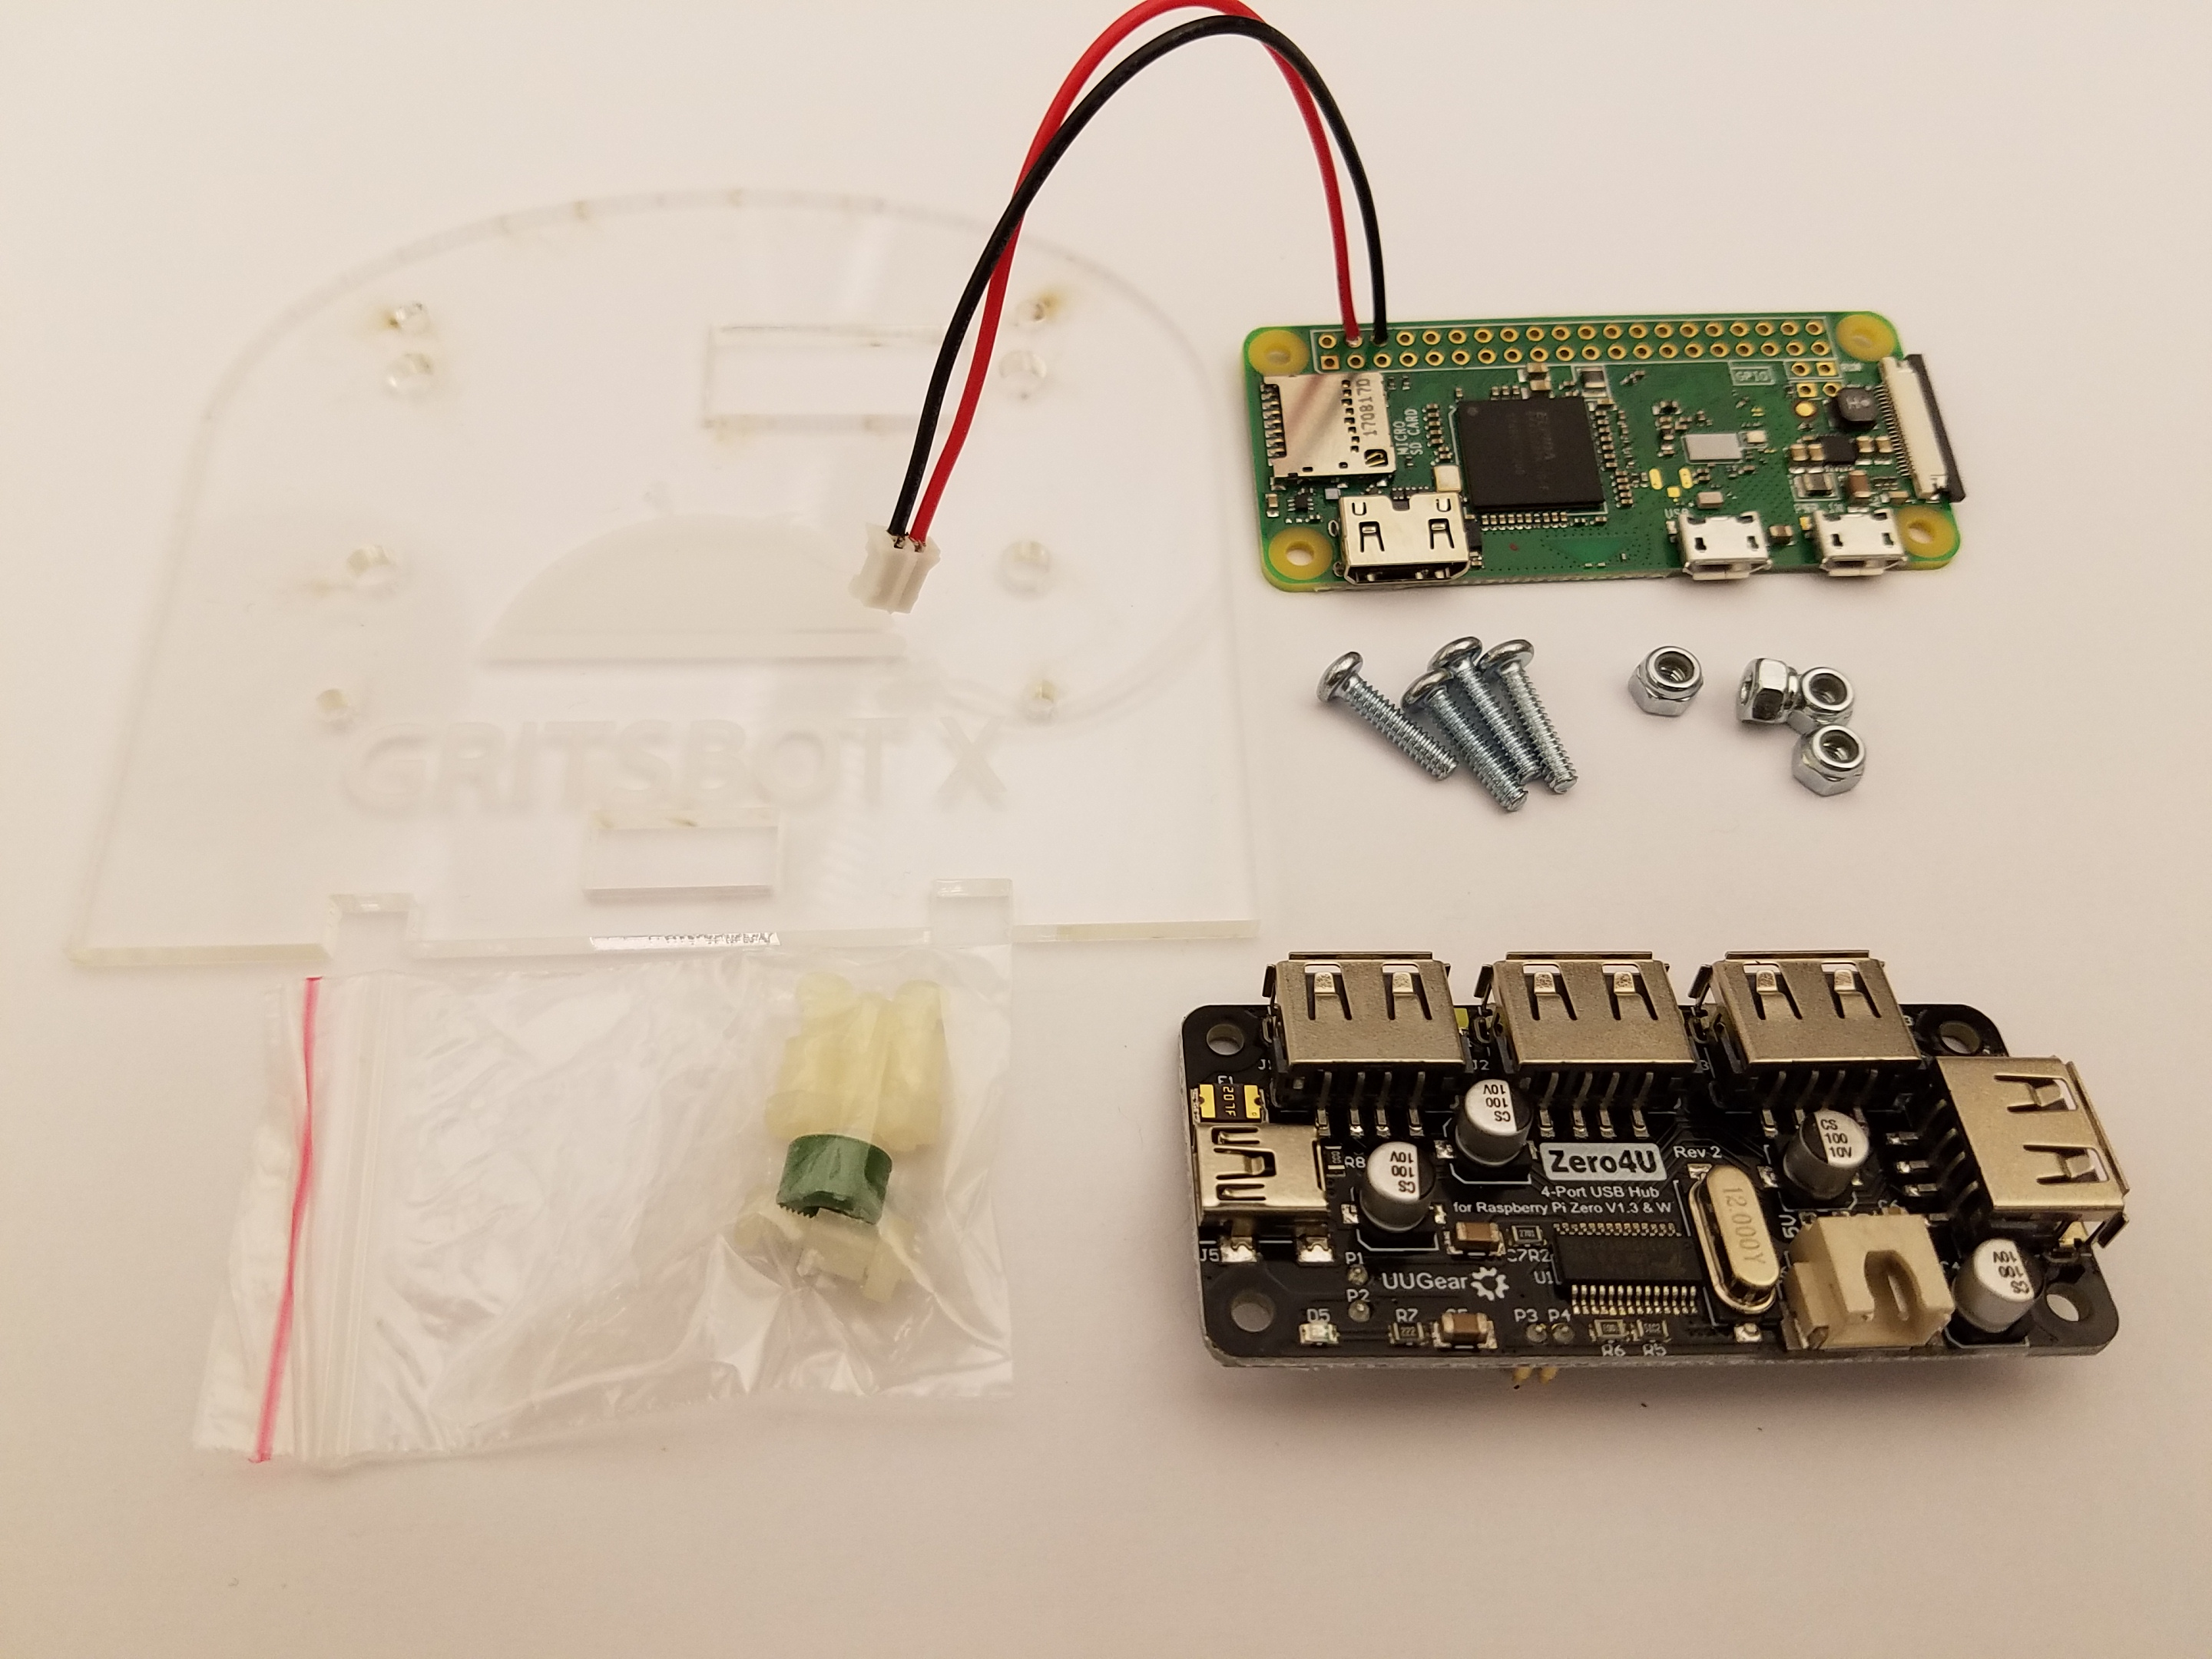
\includegraphics[width=0.65\columnwidth, keepaspectratio]{./figs/20190107_091402.jpg}
\caption{The parts required to assemble and attach the chassis cover of the GRITSBot X.}
\label{fig:topPlateMaterials}
\end{figure}
%End Top Chassis Materials  Picture

 %Begin Chassis Top Part Table
 \begin{table}[h!]
 \centering
\begin{tabular}{p{3in}c}
\rowcolor[HTML]{C0C0C0} 
\textbf{Part}  & \textbf{Number Required} 		\\
Assembled Chassis Base from \cref{sec:finishBase}		& 1	\\
\rowcolor[HTML]{C0C0C0} 
Acrylic Top Plate			& 1	\\
Raspberry Pi Zero with Soldered Leads from \cref{sec:raspberryPiLeads}	& 1	\\
\rowcolor[HTML]{C0C0C0} 
Zero4U 4-Port USB Hub	 Kit	& 1 \\
Tracking Hat				& 1 \\
\rowcolor[HTML]{C0C0C0} 
4-40, $1/2$ inch Screw	& 4  \\
4-40 Locknut	& 4\\
\rowcolor[HTML]{C0C0C0} 
4-40, $1/4$ inch Screw	& 4  \\
4-40, $5/8$ inch Male to Female Hexagonal Standoff	& 4\\
\end{tabular}
\caption{The parts required to assemble and attach the chassis cover of the GRITSBot X. \label{tab:topPlateMaterials}}
\end{table}
 %End Chassis Top Part Table

\subsubsection{Attaching the Peripheral Circuit Boards to the Top Chassis}
\label{sec:attachZero4U}

pictured in \cref{fig:topPlateMaterials} and

The first step in this assembly is to attach the Raspberry Pi Zero W \cite{raspberryPiZeroW} to the Zero4U 4-port USB hub \cite{zero4u}. This allows the Raspberry Pi Zero W to connect to the Teensy using a readily available on-the-go (OTG) USB cable as well as extend its wireless communication capabilities with a USB Wi-Fi antenna or other peripherals with limited current draw.

%Top Chassis Materials Picture
\begin{figure}[h!]
\centering
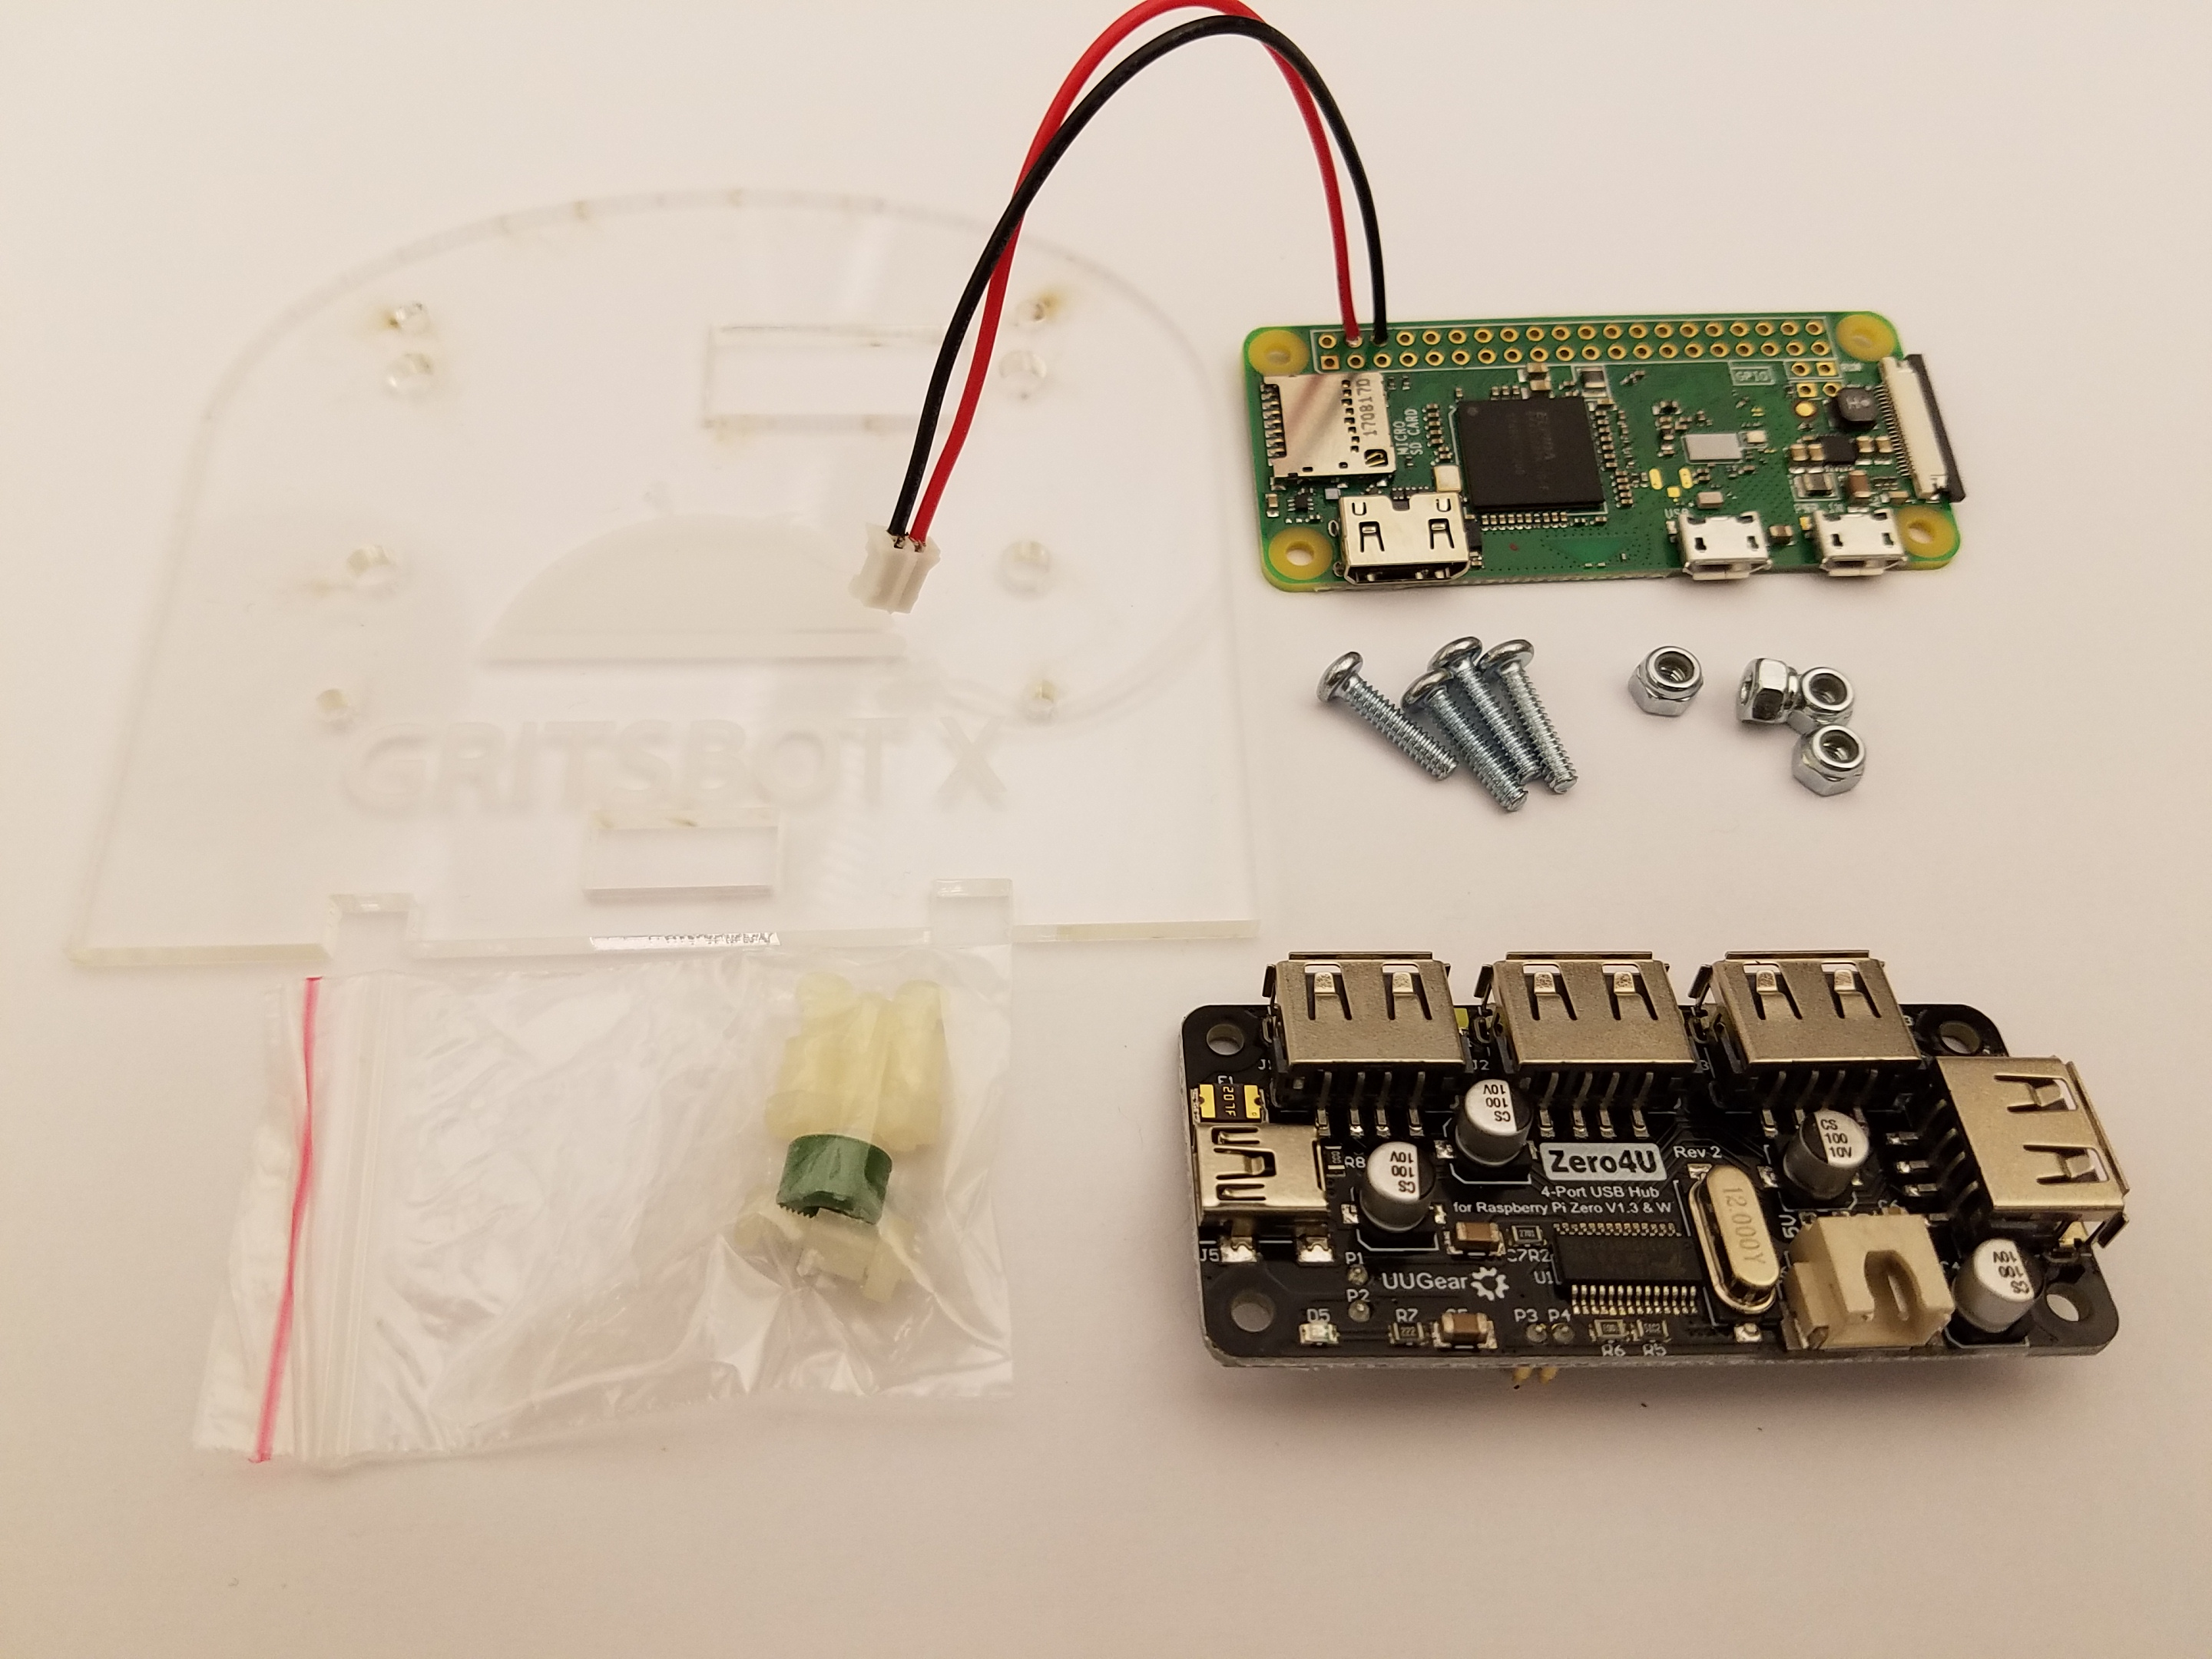
\includegraphics[width=0.65\columnwidth, keepaspectratio]{./figs/20190107_091402.jpg}
\caption{The parts required to assemble and attach the chassis cover of the GRITSBot X.}
\label{fig:topPlateMaterials}
\end{figure}
%End Top Chassis Materials  Picture

The parts needed for this are pictured in \cref{fig:topPlateMaterials}. Insert the four 4-40, $1/2$ inch screws through the Zero4U such that the head of the screw is on the same side as the USB ports. Slide the four plastic spacers provided with  the Zero4U kit onto the screws. Slide the green ferrite ring around the two pins that are parallel to the long edge of the board \cite{zero4uRing}. Place the screws through the four wider holes in the acrylic top plate. The Zero4U board should be on the top of the acrylic plate (the side with the etching or the side with the off center rectangular cut on the right with the curved surface being the front). Finally, place the Raspberry Pi Zero W on the other side and thread the screws through the corresponding four screw holes. The metal pins from the Zero4U should align with the exposed pads on the opposite side of the USB ports on the Raspberry Pi. If done correctly, the assembly should look like \cref{fig:topChassisAssembled}.

%Chassis Top Assembly Picture
\begin{figure}[h!]
\centering
\subfloat[\label{fig:topAttachPCB} Top view of the chassis cover.]{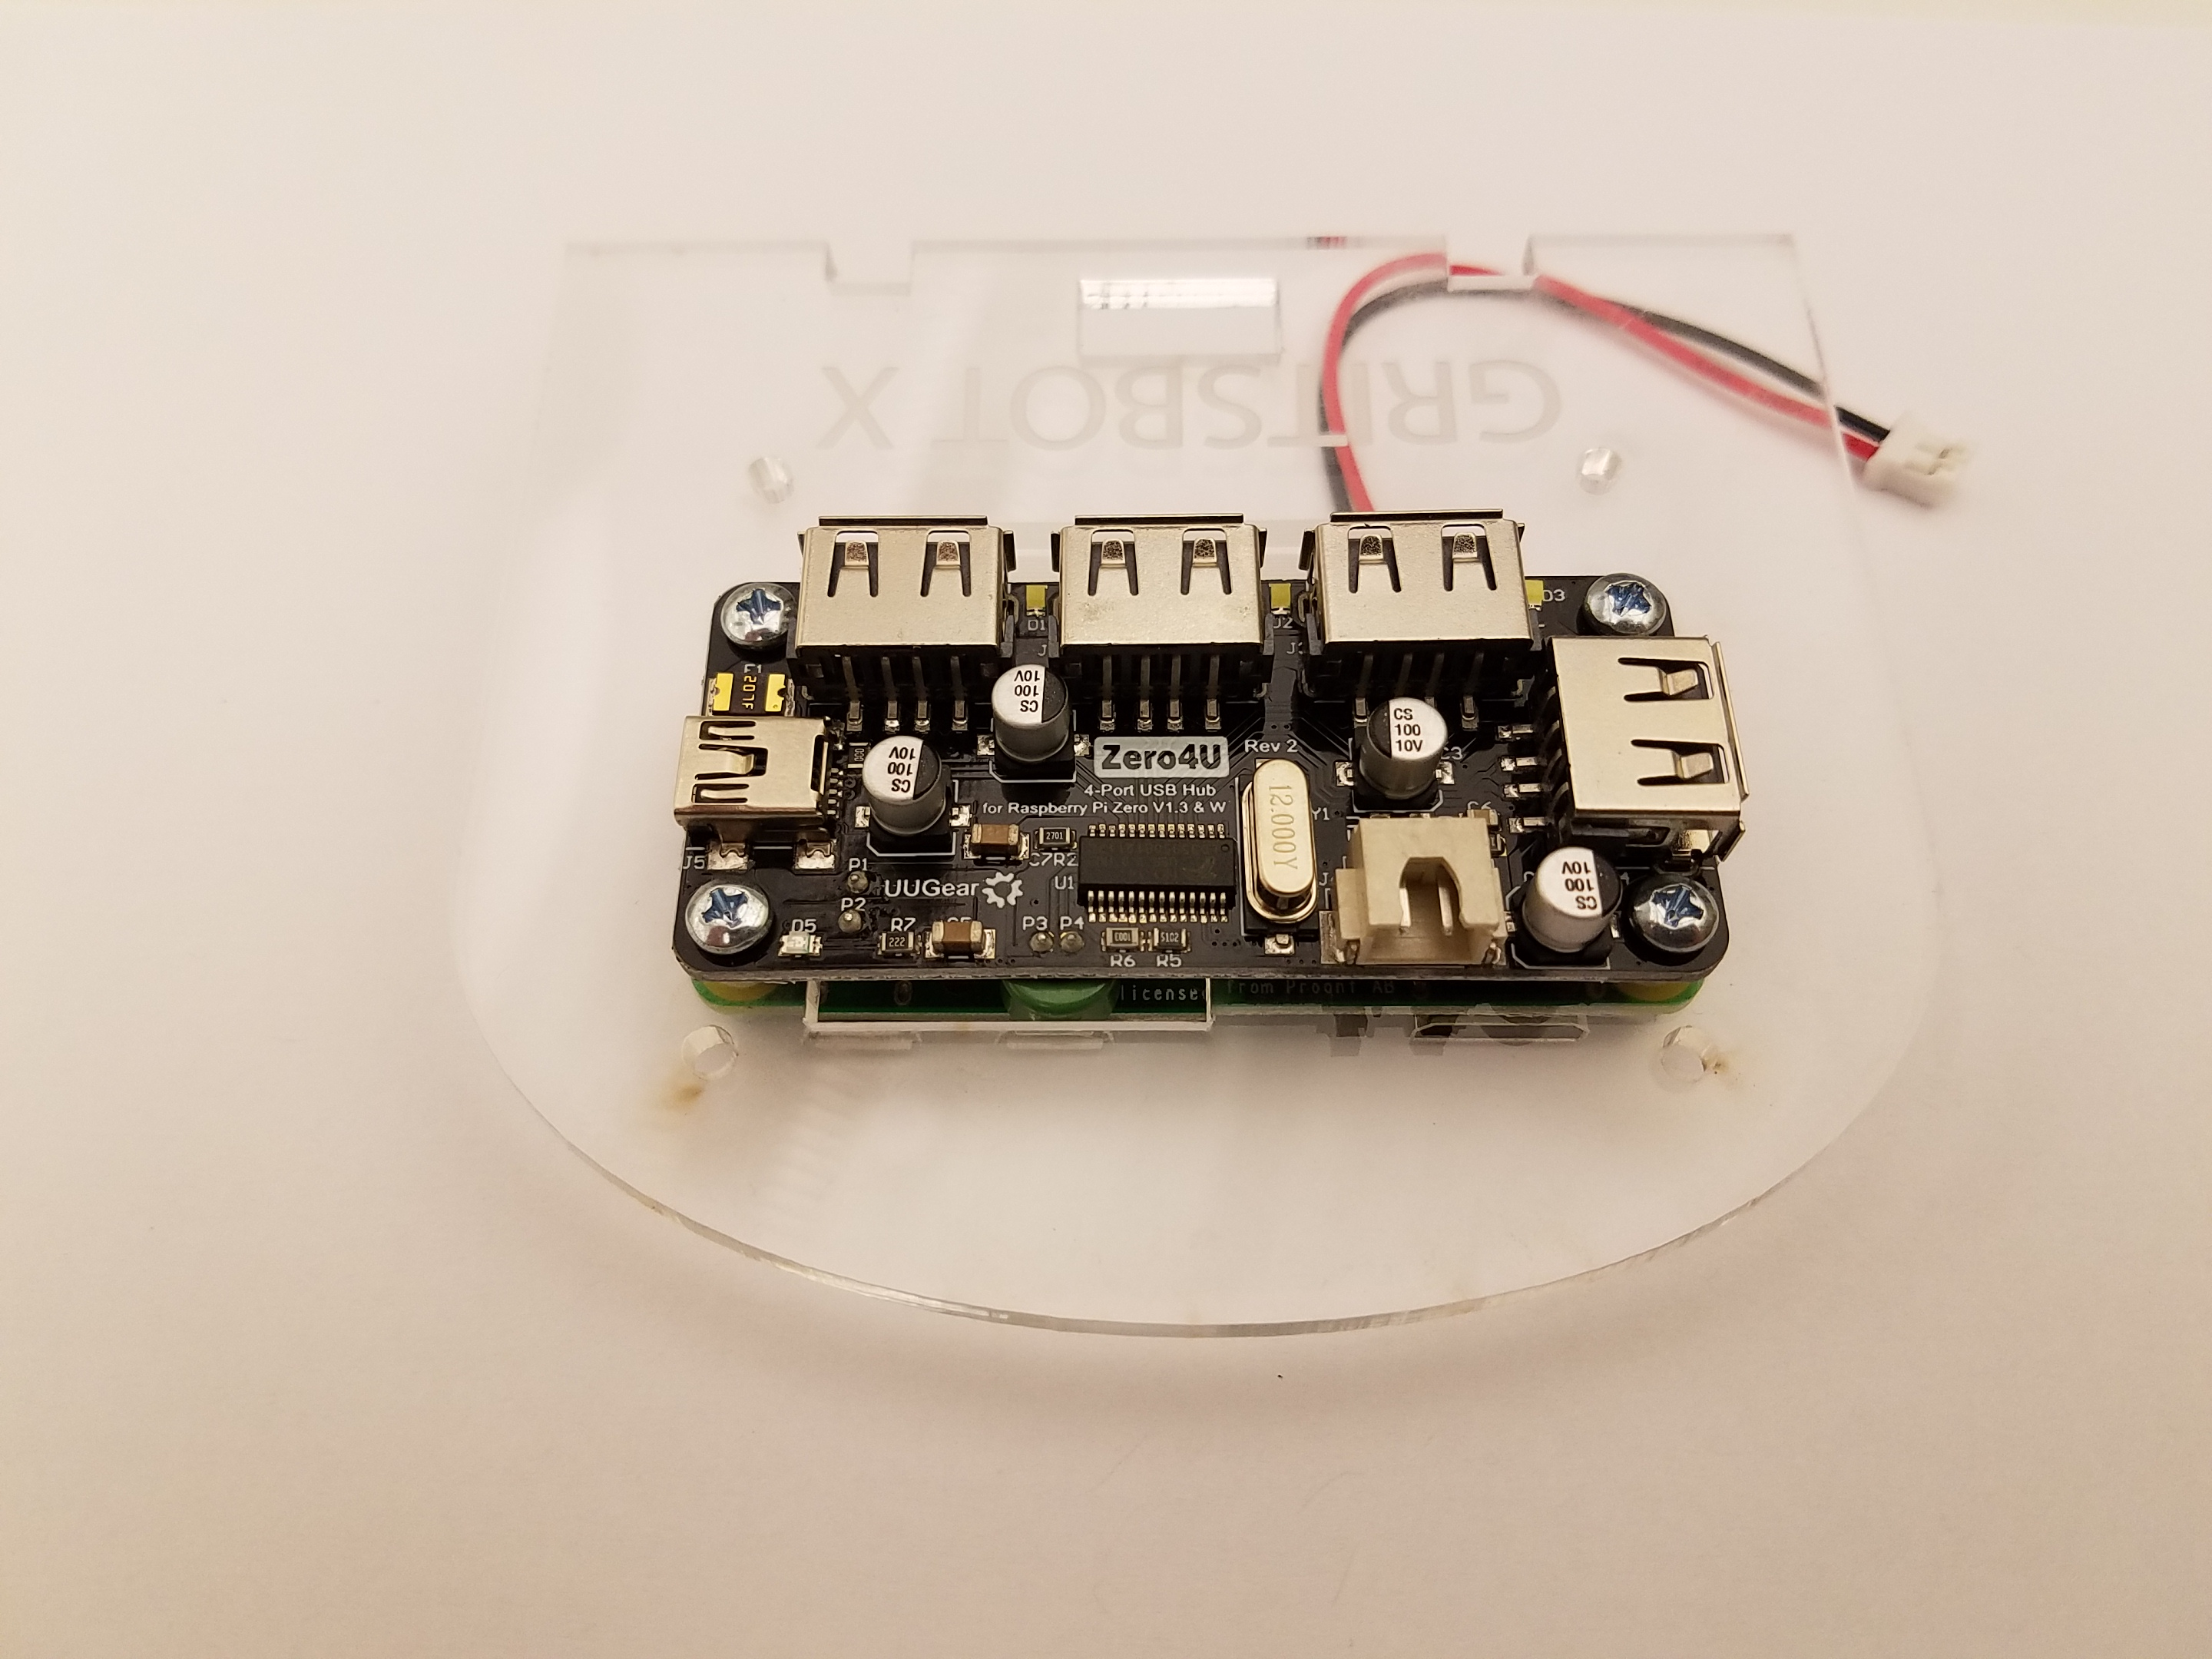
\includegraphics[width=0.45\columnwidth, keepaspectratio]{./figs/20190107_091939.jpg}}
\hfill
\subfloat[\label{fig:backAttachPCB} Bottom view of the chassis cover.]{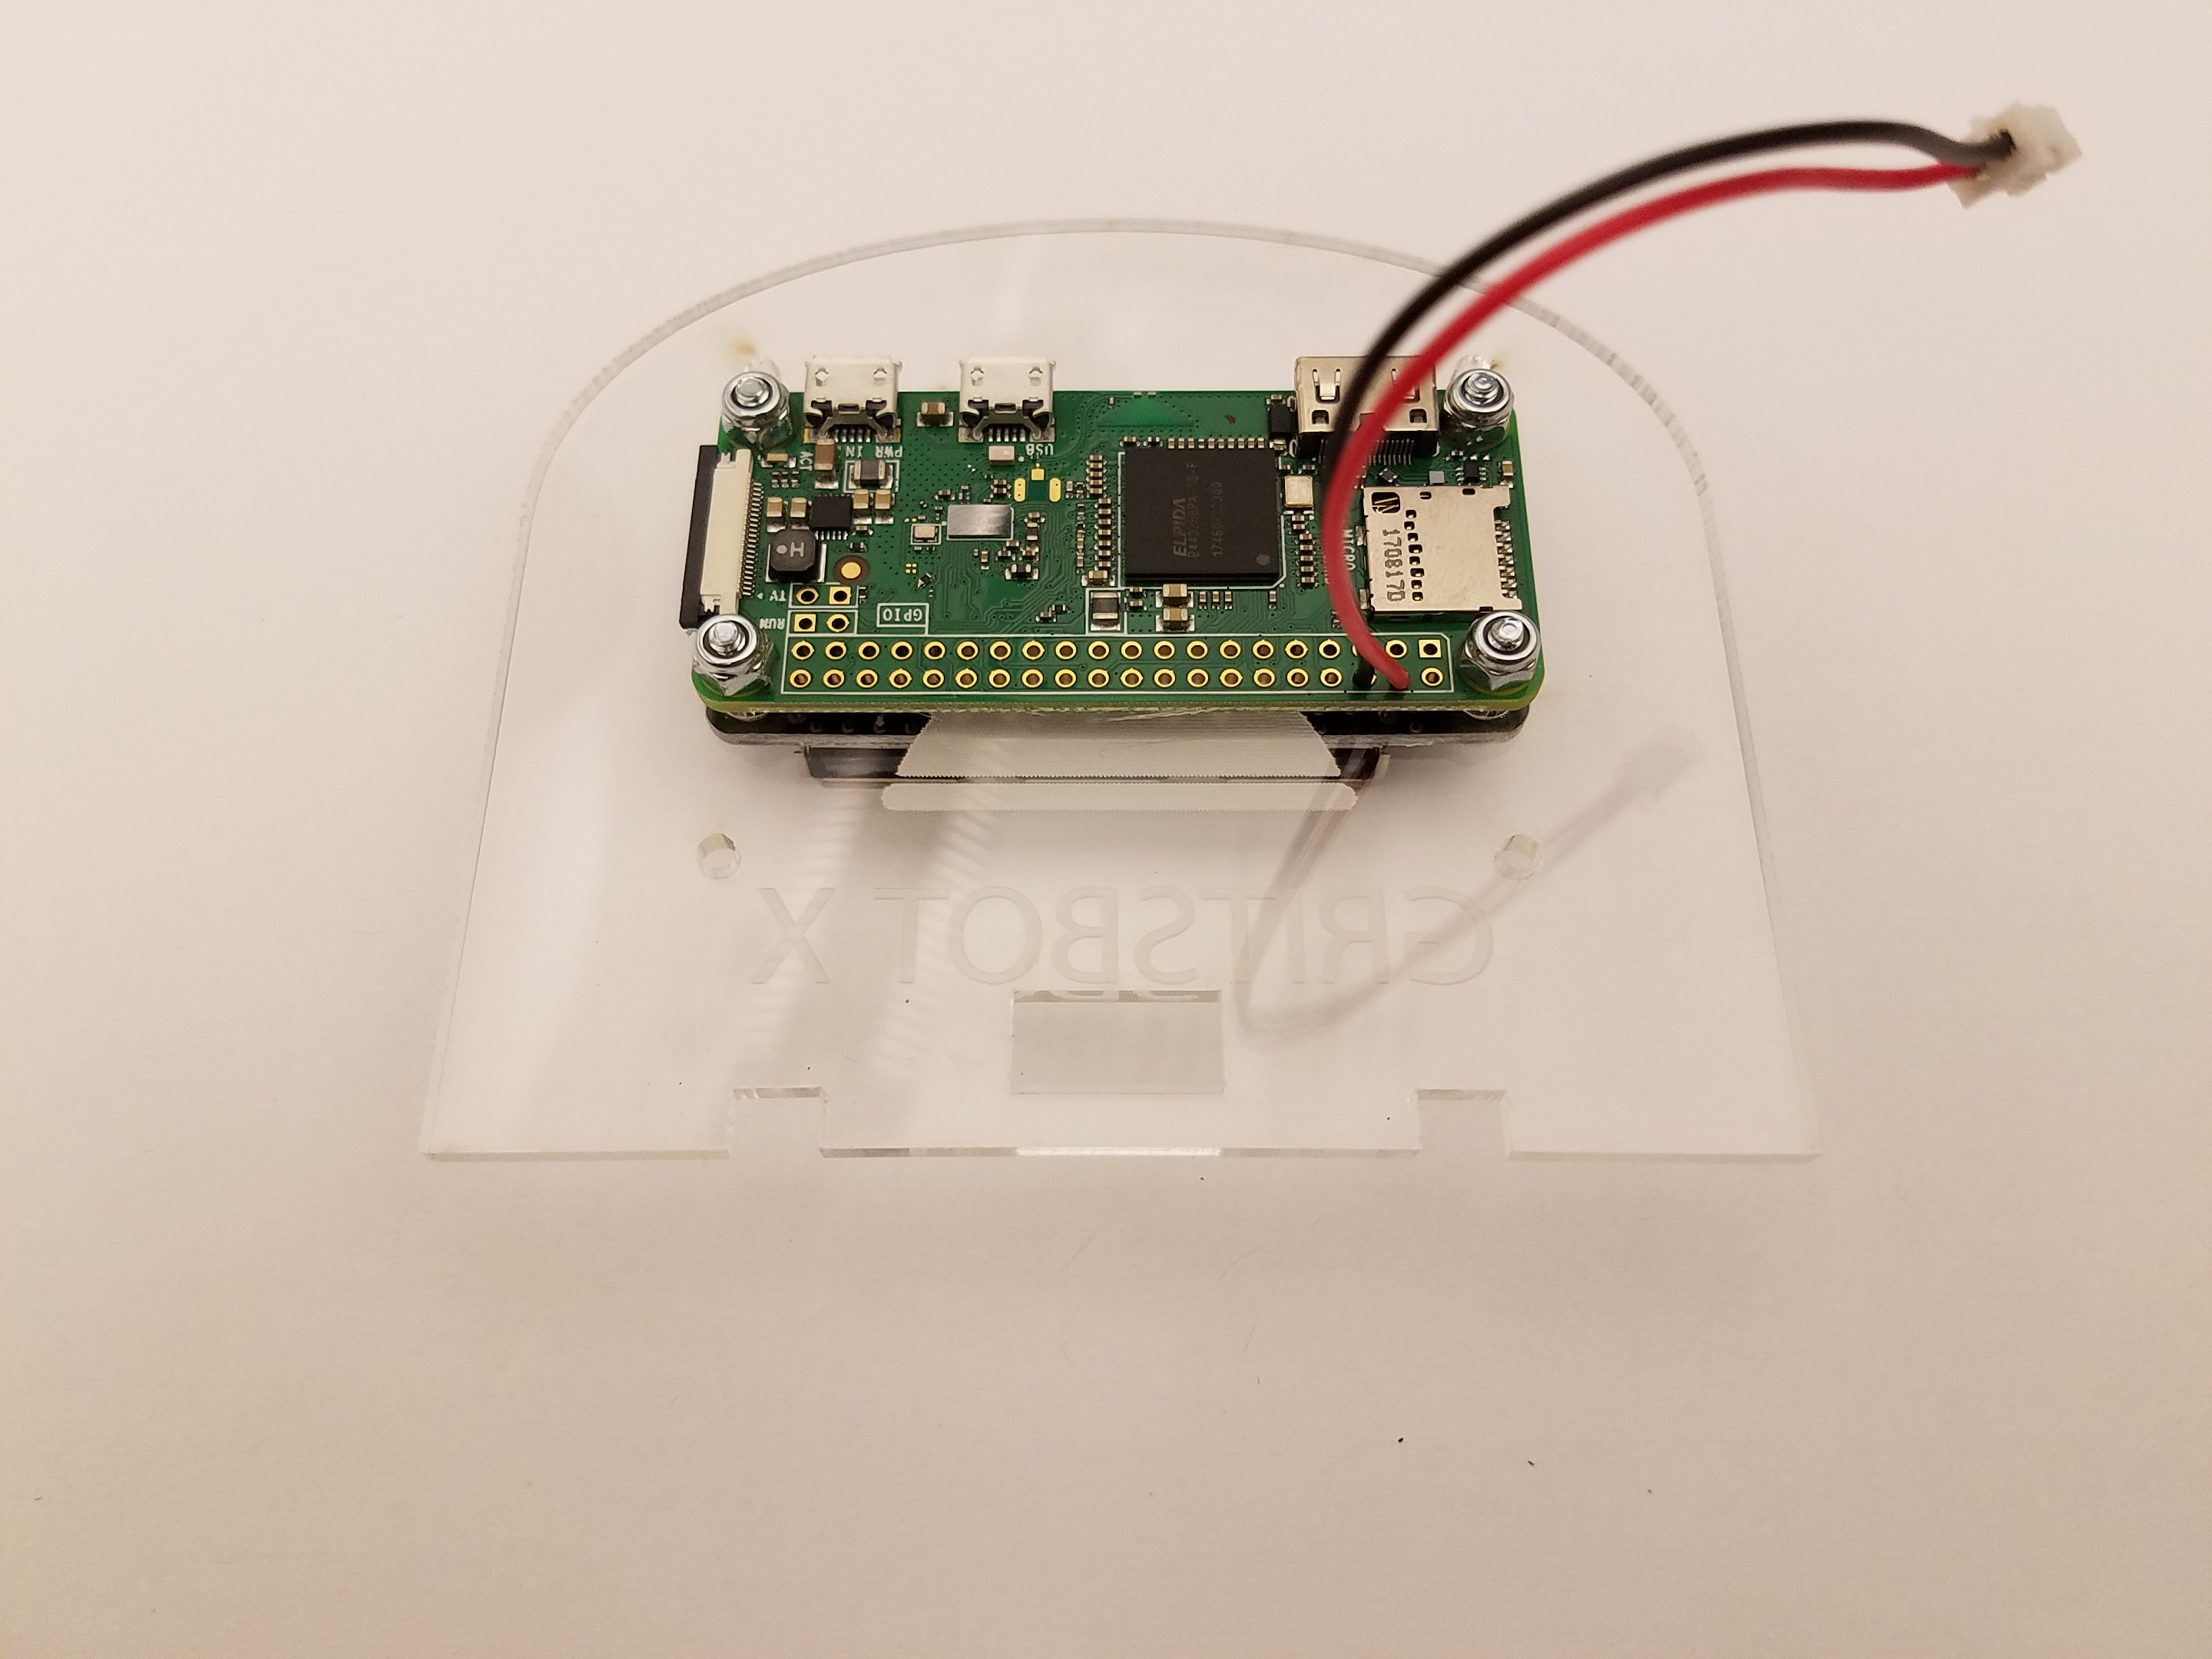
\includegraphics[width=0.45\columnwidth, keepaspectratio]{./figs/20190107_091929.jpg}}\\
\caption{The GRITSBot X chassis cover.}
\label{fig:topChassisAssembled}
\end{figure}
%End Chassis Top Assembly Picture

\subsubsection{Attaching the Chassis Cover to the Base Chassis}
\label{sec:attachChassisTop}

The final step is to attach this chassis cover to the base built in \cref{sec:finishBase}. The parts needed for this are pictured in \cref{fig:finalChassisMaterials}.

%Top Chassis Materials Picture
\begin{figure}[h!]
\centering
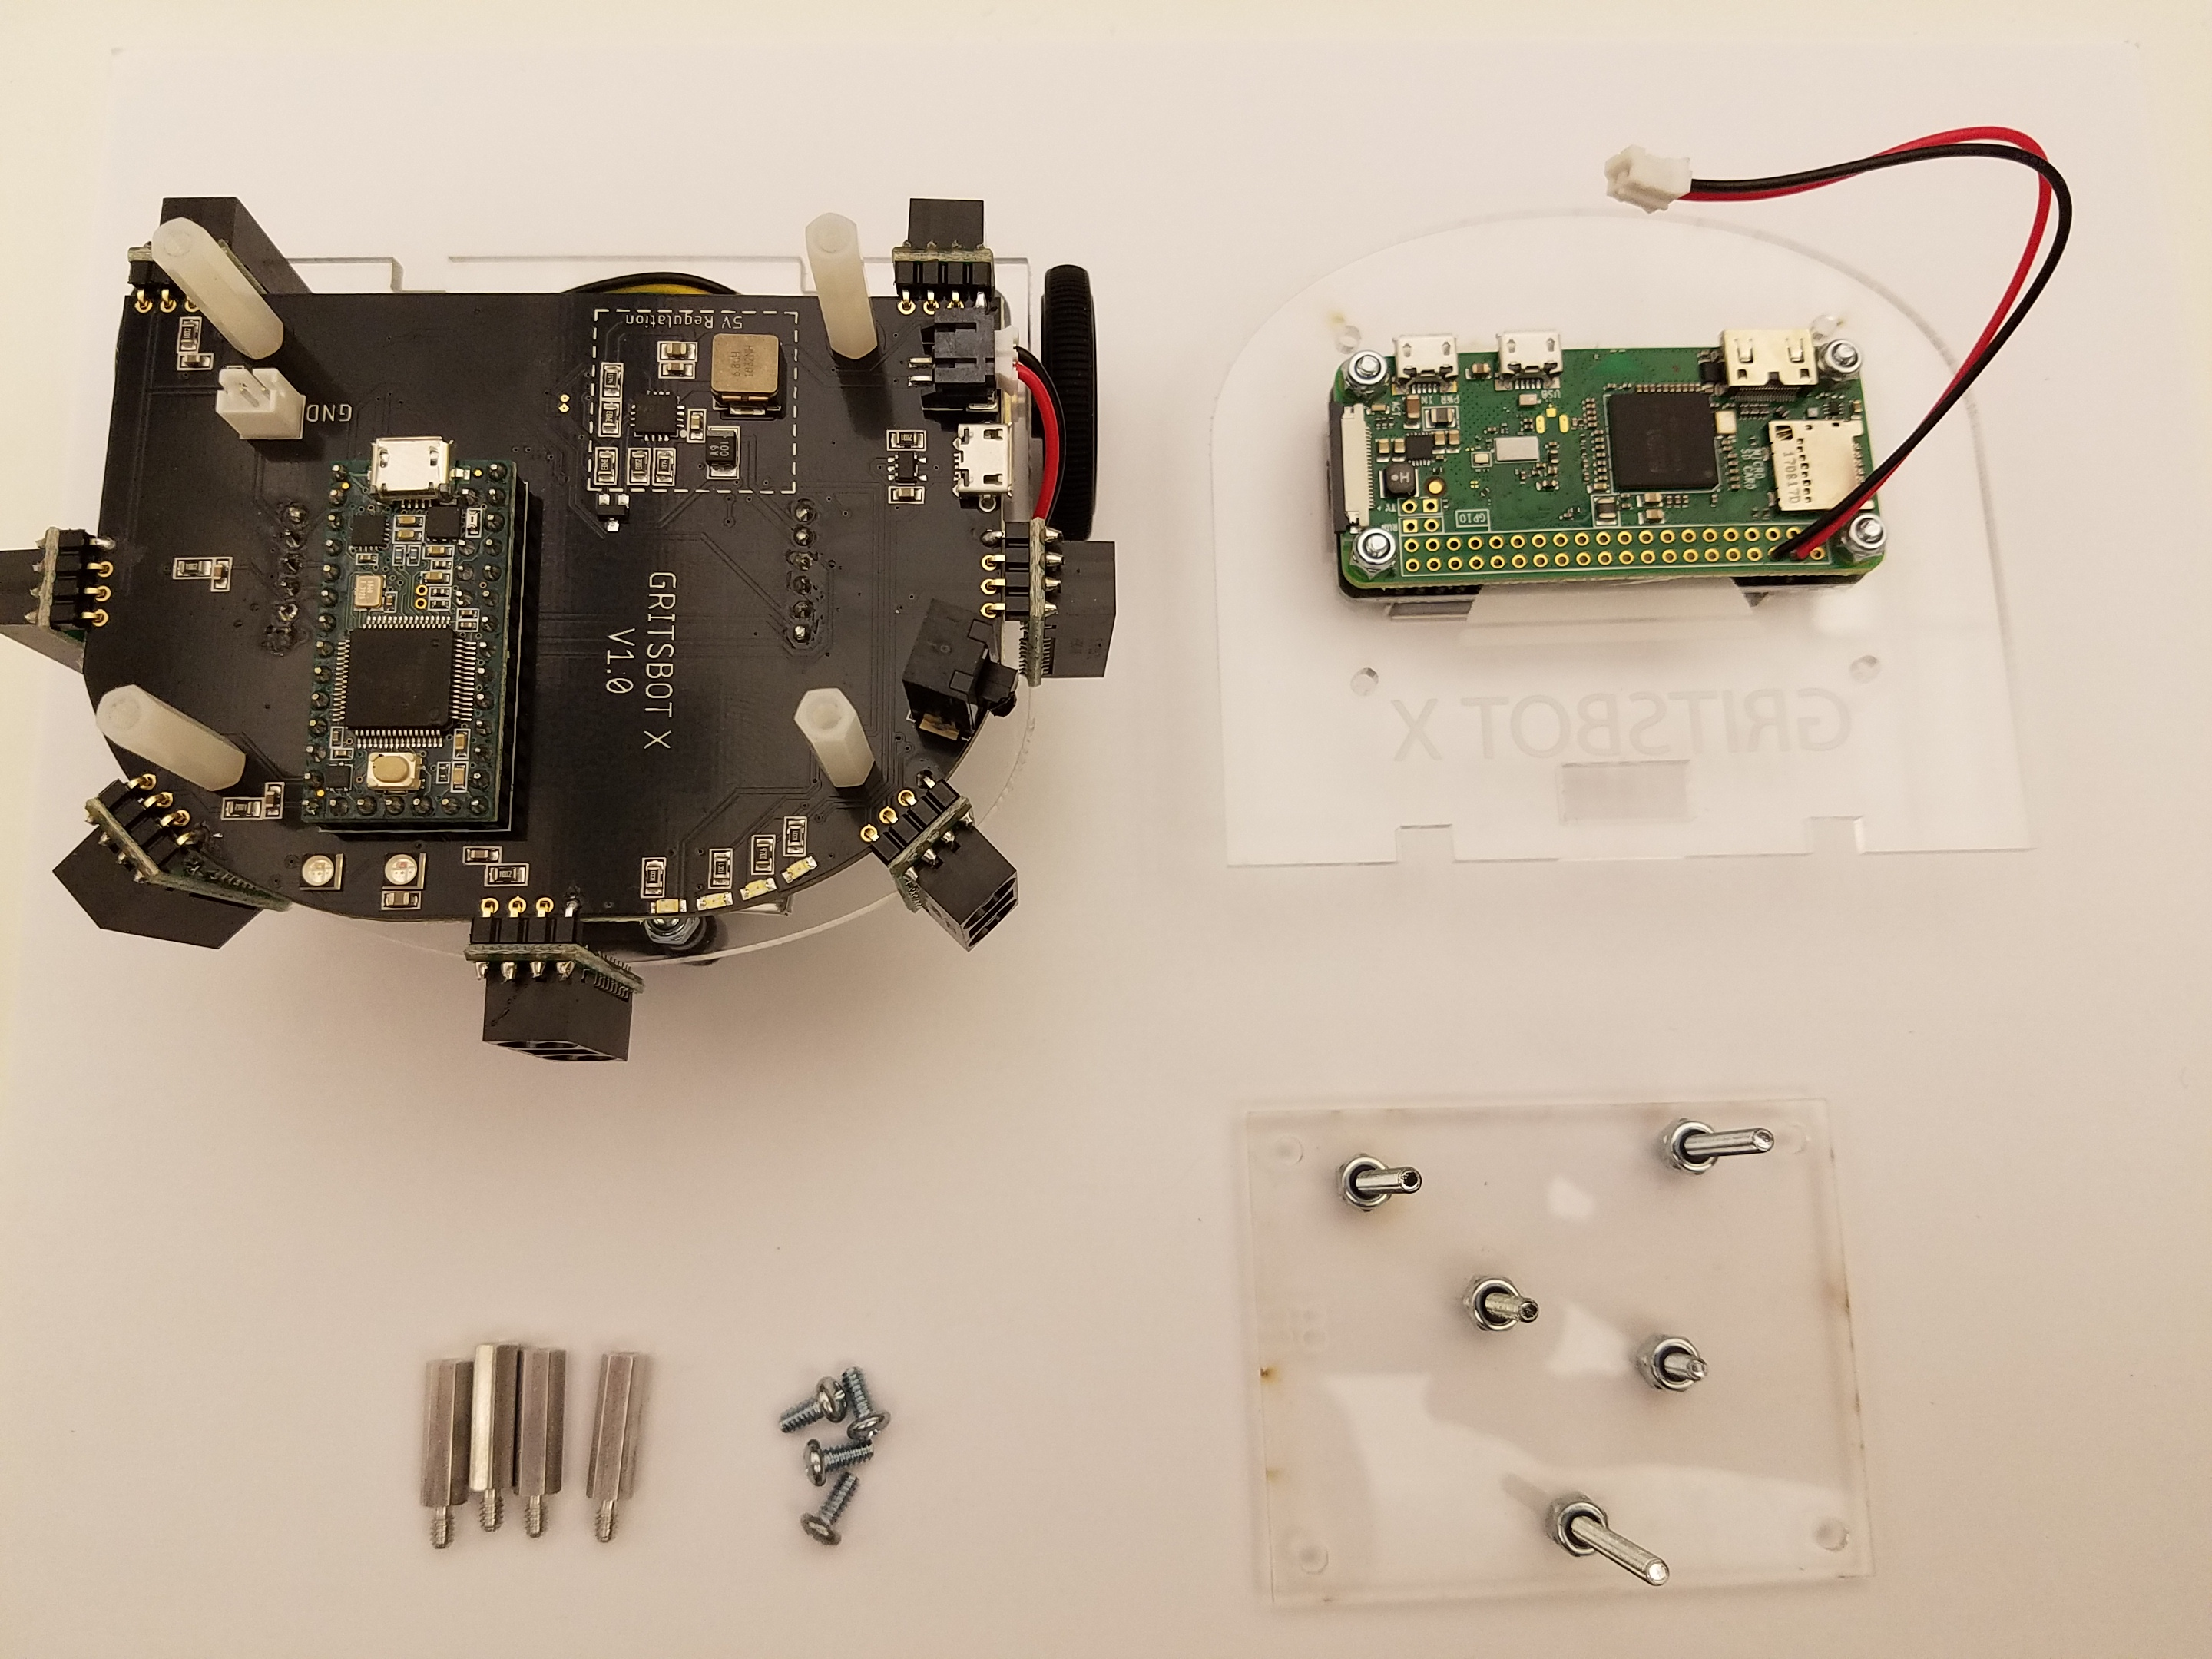
\includegraphics[width=0.65\columnwidth, keepaspectratio]{./figs/20190107_092608.jpg}
\caption{The parts required to the chassis cover to the base of the GRITSBot X.}
\label{fig:finalChassisMaterials}
\end{figure}
%End Top Chassis Materials  Picture

First, insert the power jumper from the Raspberry Pi Zero into the JST connector in the lower right of main PCB of the GRITSBot X. It should only fit one way but can be forced in the wrong way. {\color{red}{Note}}, if this wire is plugged in the wrong way with the robot powered on, the Raspberry Pi Zero W will probably be destroyed and other components on the PCB can also be destroyed. Make sure the plastic tab on the end of the jumper cable aligns with the hole on the PCB. \cref{fig:pluggedPi} pictures the jumper plugged into the PCB correctly.

%Plugged in Pi Picture
\begin{figure}[h!]
\centering
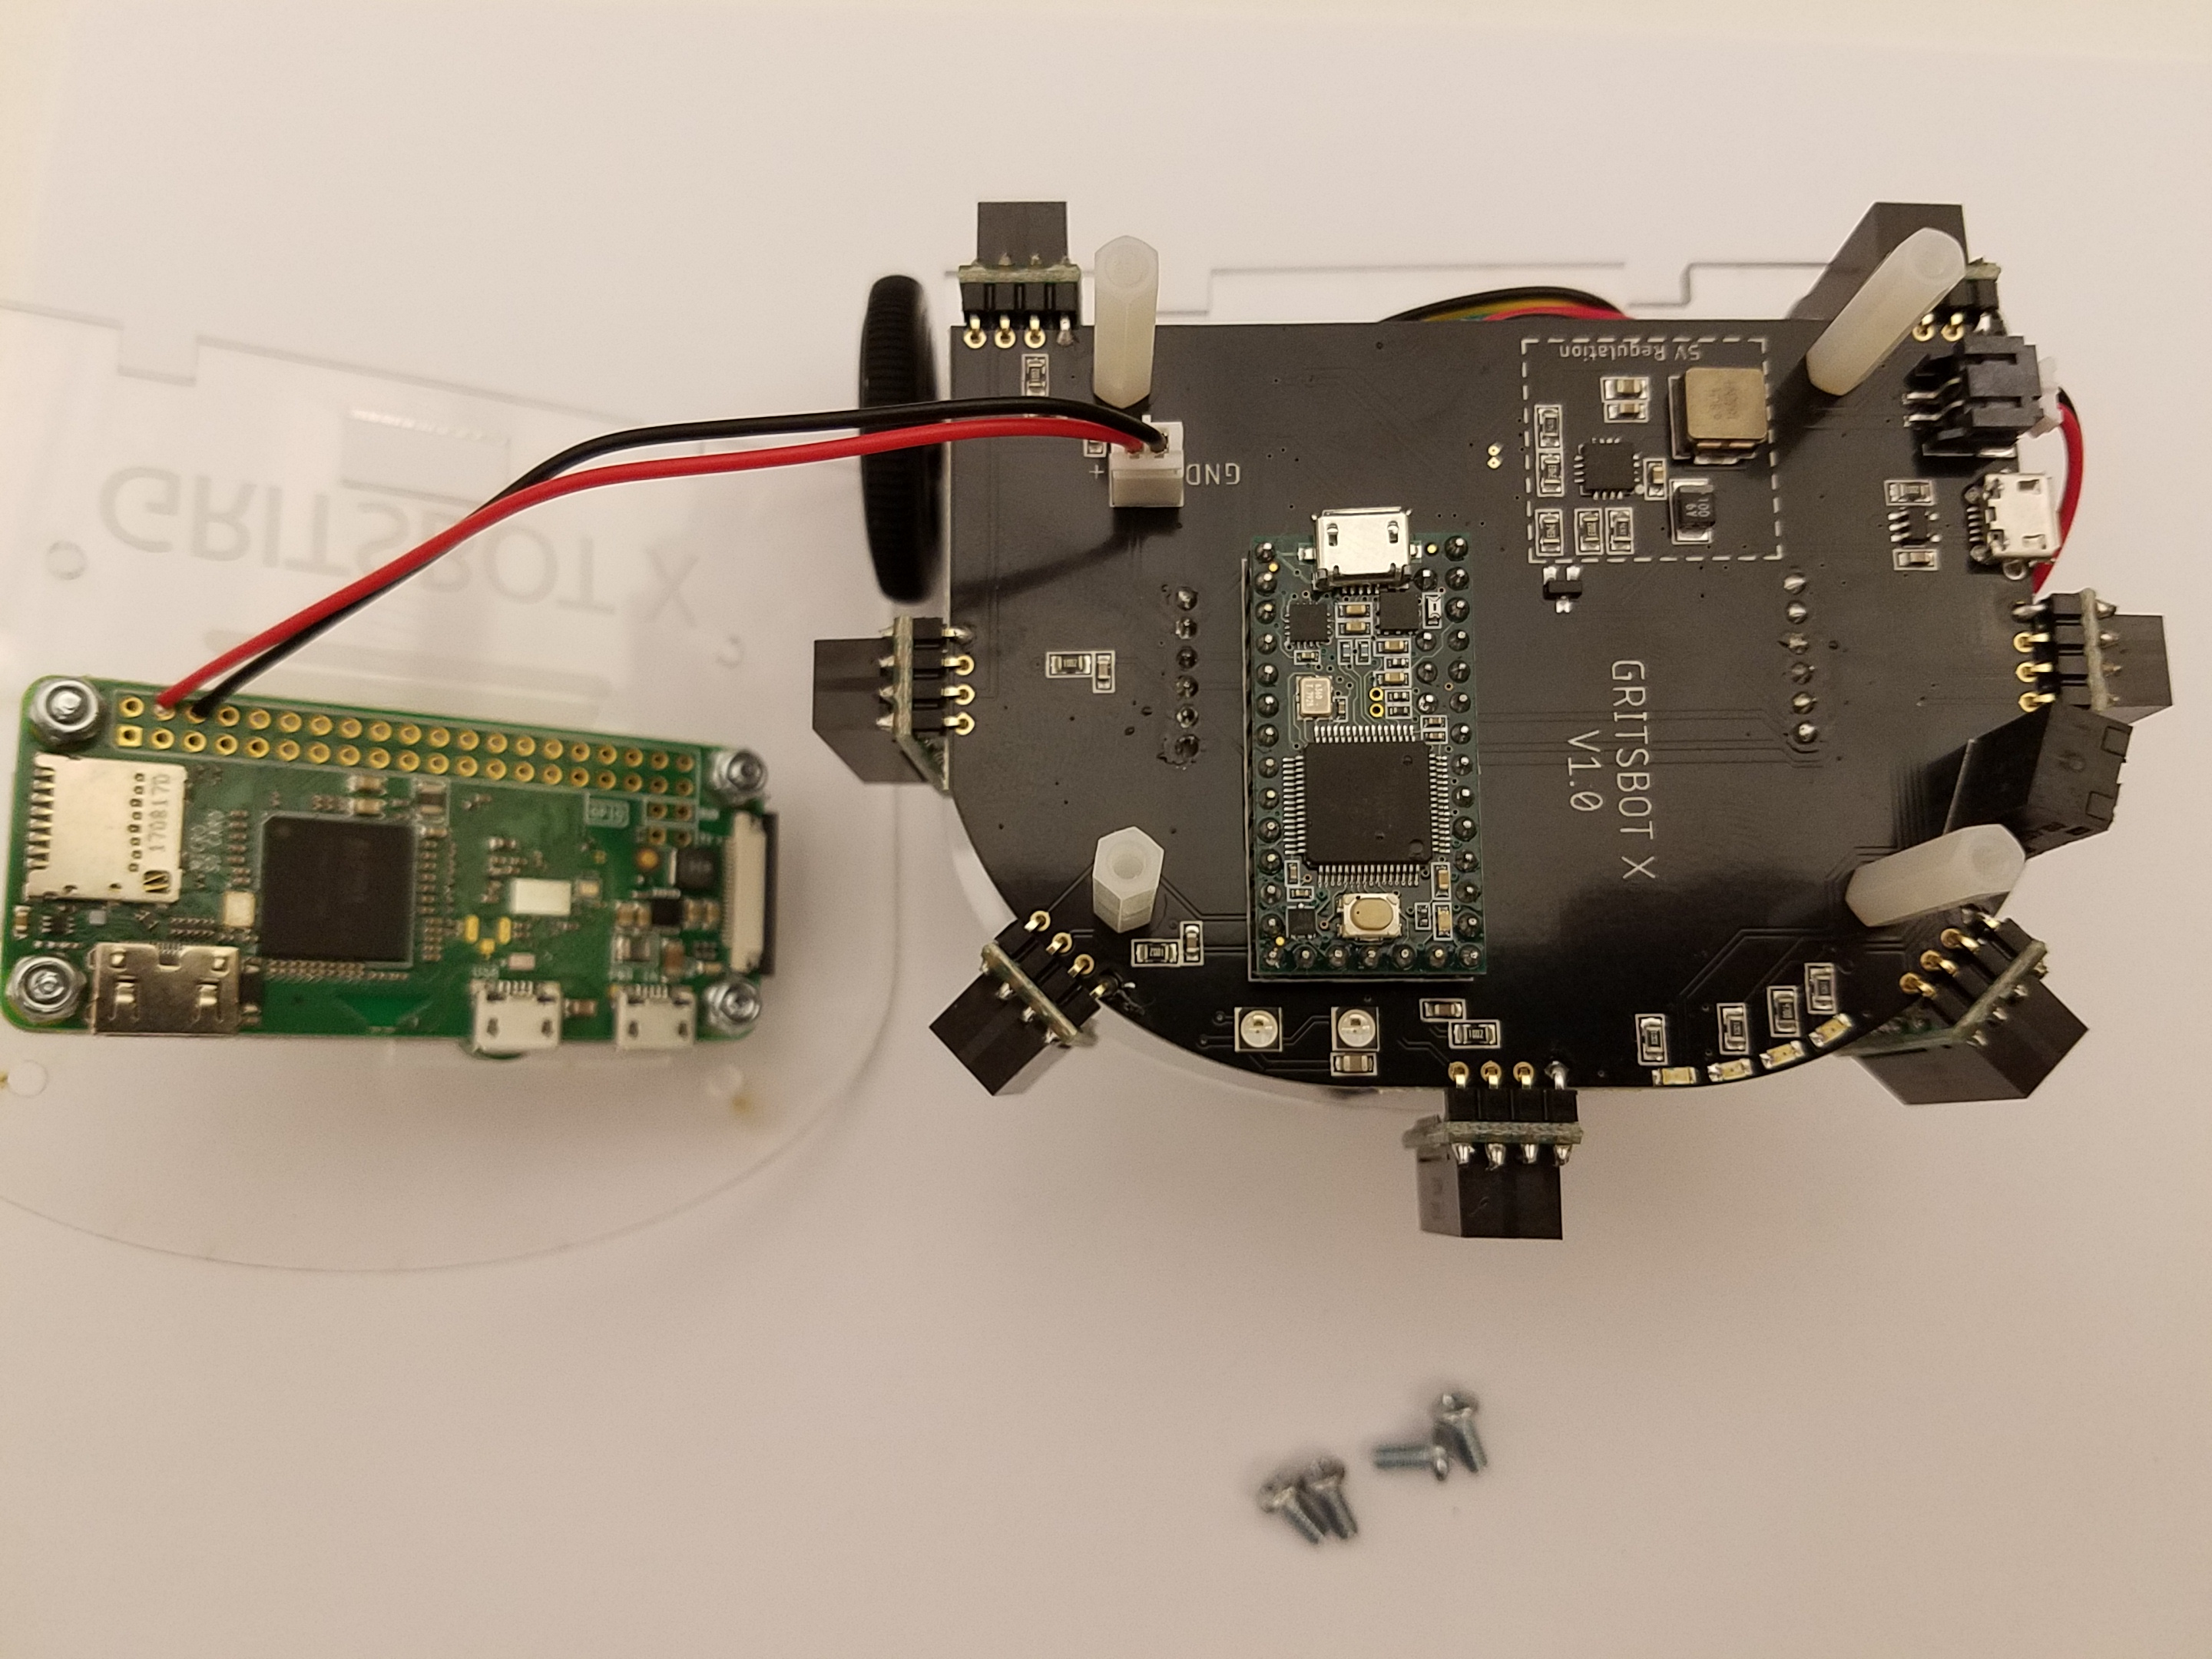
\includegraphics[width=0.65\columnwidth, keepaspectratio]{./figs/20190107_092139.jpg}
\caption{The Raspberry Pi Zero W correctly plugged into the main PCB of the GRITSBot X.}
\label{fig:pluggedPi}
\end{figure}
%End Plugged in Pi  Picture

After plugging in the Raspberry Pi Zero W place the top acrylic onto the standoffs and secure it with the four 4-40, $5/8$ inch male to female hexagonal standoff. The outer shape of the top plate should align with the bottom plate and the Raspberry Pi Zero W should be on the interior of the robot. If done correctly, the robot without its finishing touches should look like \cref{fig:nearFinalChassis}.

%Final Chassis Picture
\begin{figure}[h!]
\centering
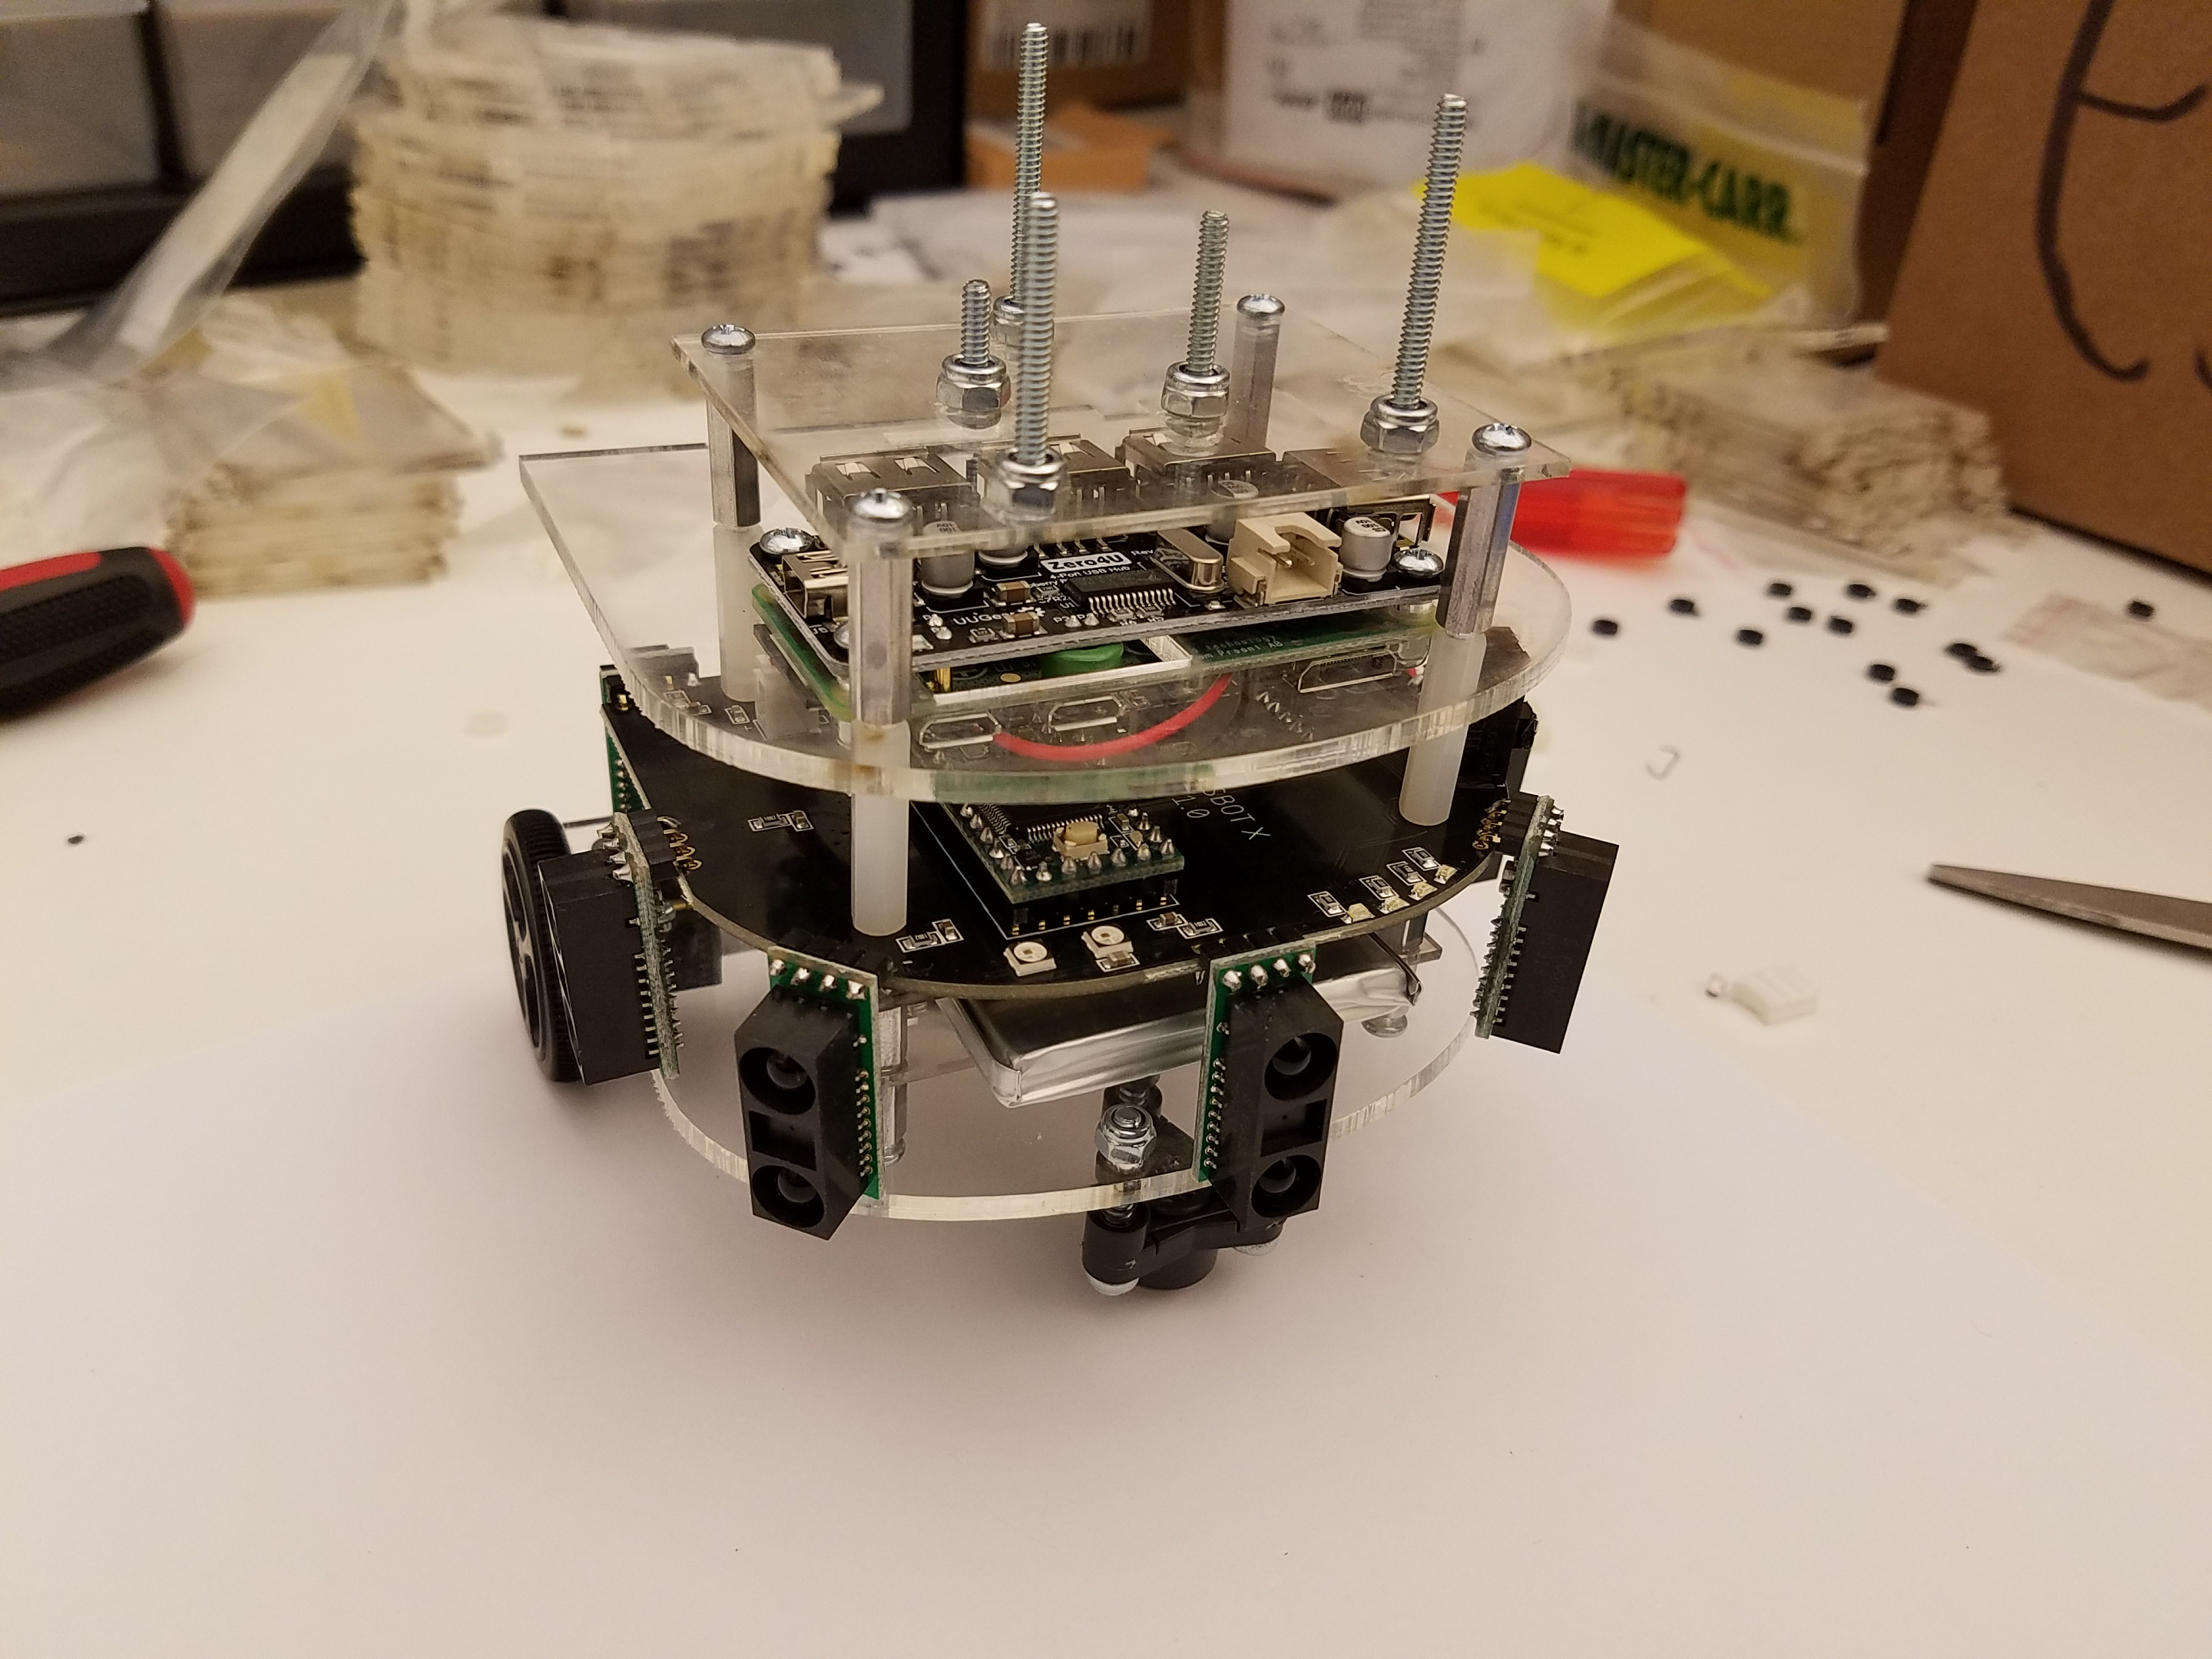
\includegraphics[width=0.65\columnwidth, keepaspectratio]{./figs/20190107_092811.jpg}
\caption{The chassis base with chassis cover attached.}
\label{fig:nearFinalChassis}
\end{figure}
%End Plugged in Pi  Picture

\subsection{The Final Touches}
\label{sec:finalTouch}

\subsubsection{Assembly Steps}
\label{sec:finalAssembly}

\begin{enumerate}
\item Gathe the required materials (\cref{sec:finalMaterials}).
\item Plug in the periferal electronics (\cref{sec:plugIn}).
\item Attach the charging plate (\cref{sec:chargingPlate}).
\item CELEBRATE FINISHING! (\cref{sec:CELEBRATE}).
\end{enumerate}

\subsubsection{Required Materials}
\label{sec:finalMaterials}

The final step is to connect the Teensy and Raspbeery Pi Zero W so they can communicate over serail, add a Wi-Fi antenna to boost signal reception, and attach the charging plate. A picture of the required materials is in \cref{fig:finalMaterials} with a table listing them in \cref{tab:finalMaterials}.

%Final Matrials Picture
\begin{figure}[h!]
\centering
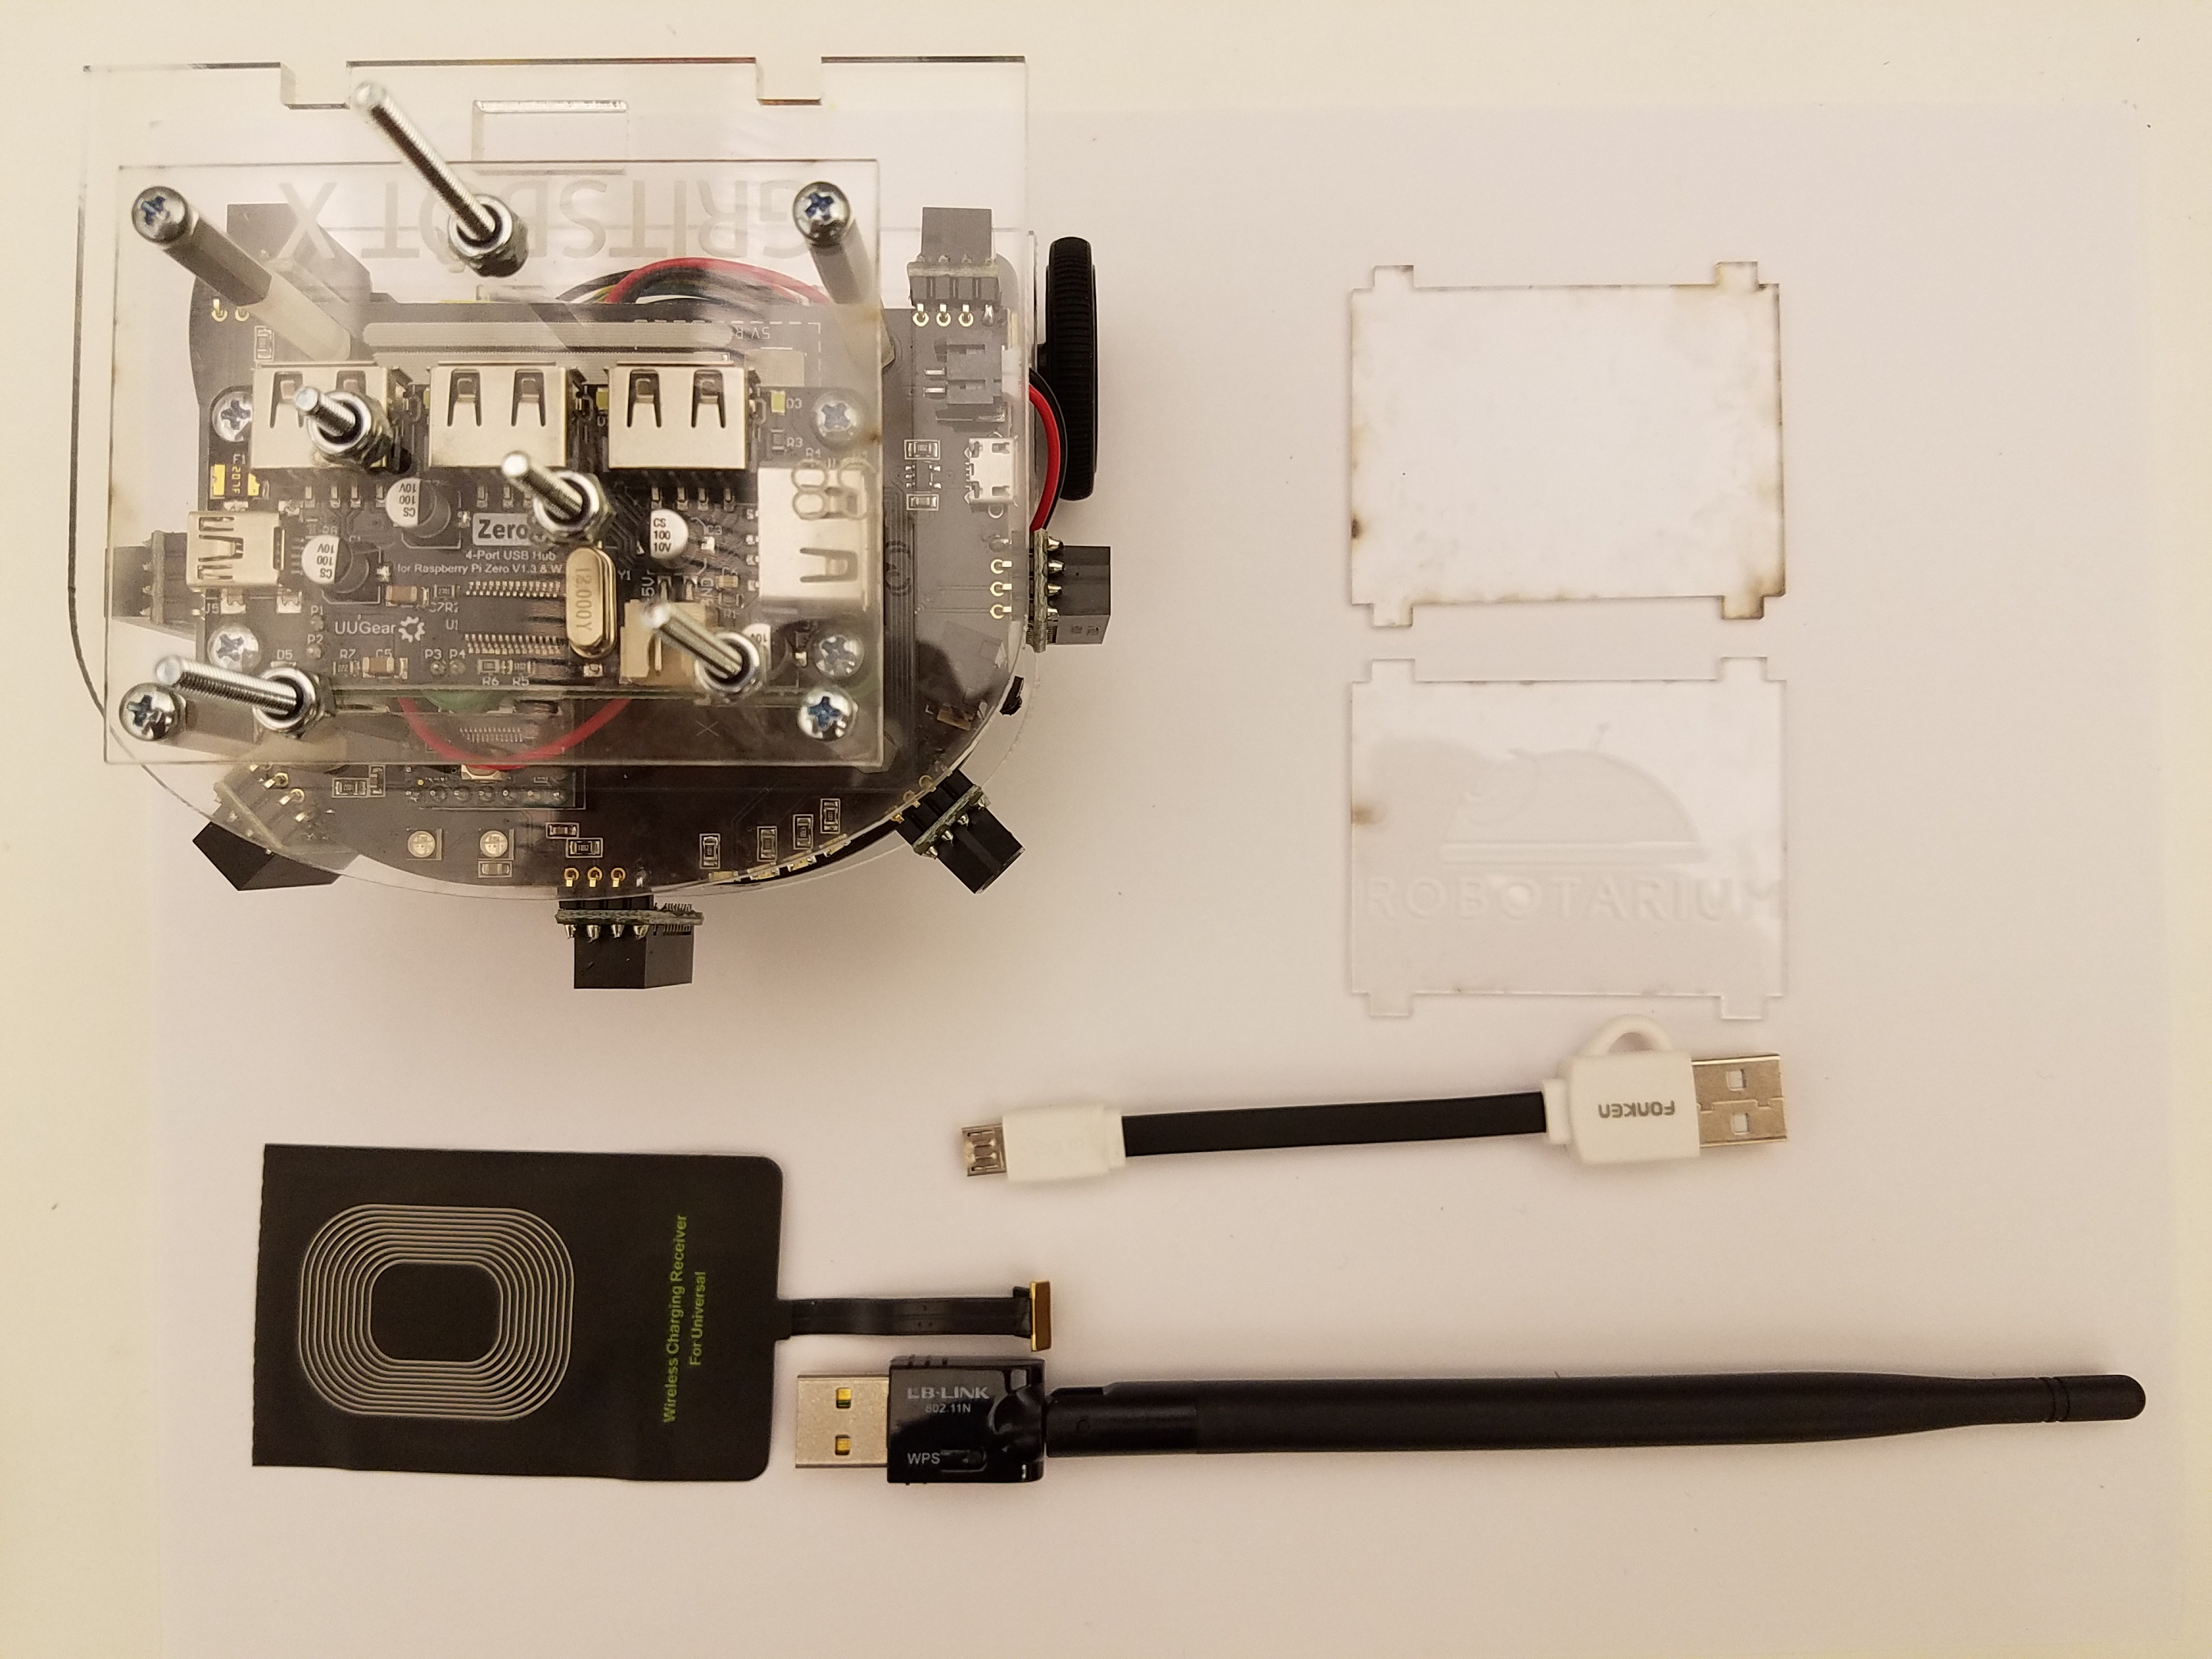
\includegraphics[width=0.65\columnwidth, keepaspectratio]{./figs/20190110_132826.jpg}
\caption{The materials needed to finish the assembly of the GRITSBot X.}
\label{fig:finalMaterials}
\end{figure}
%End Materials  Picture

 %Begin Final Part Table
 \begin{table}[h!]
 \centering
\begin{tabular}{p{3in}c}
\rowcolor[HTML]{C0C0C0} 
\textbf{Part}  & \textbf{Number Required} 		\\
Assembled GRITSBot X from \cref{sec:topPlate}		& 1	\\
\rowcolor[HTML]{C0C0C0} 
Acrylic Charging Back Plate			& 1	\\
Acrylic Charging Front Plate		& 1	\\
\rowcolor[HTML]{C0C0C0} 
Digiyes Qi Charging Reciever	& 1 \\
Short Micro USB Noodle Cable				& 1 \\
\rowcolor[HTML]{C0C0C0} 
LB-Link Wireless USB Adapter	& 1  \\
\end{tabular}
\caption{The parts required to finish the assmbly of the GRITSBot X. \label{tab:finalMaterials}}
\end{table}
 %End Final Part Table

\subsubsection{Attaching Periferal Electronics}
\label{sec:plugIn}

First connect the short micro USB noodle cable between the middle usb port on top of the robot and the micro USB port on the Teensy board inside the robot (\cref{fig:microUSB}). Next insert the micro usb connector of the Digiyes Qi charging receiver into the connector next to the battery connection on the PCB (\cref{fig:qiCharger}). You robot should resemble that in \cref{fig:attachedElectronics} at this point. You may now insert the LB-Link wireless USB adapter into one of the slots next to the micro USB noodle cable.

%Electronics Plugged in Picture
\begin{figure}[h!]
\centering
\subfloat[\label{fig:microUSB} The micro USB cable connecting the Rapsberry Pi (through the Zero4U) and Teensy.]{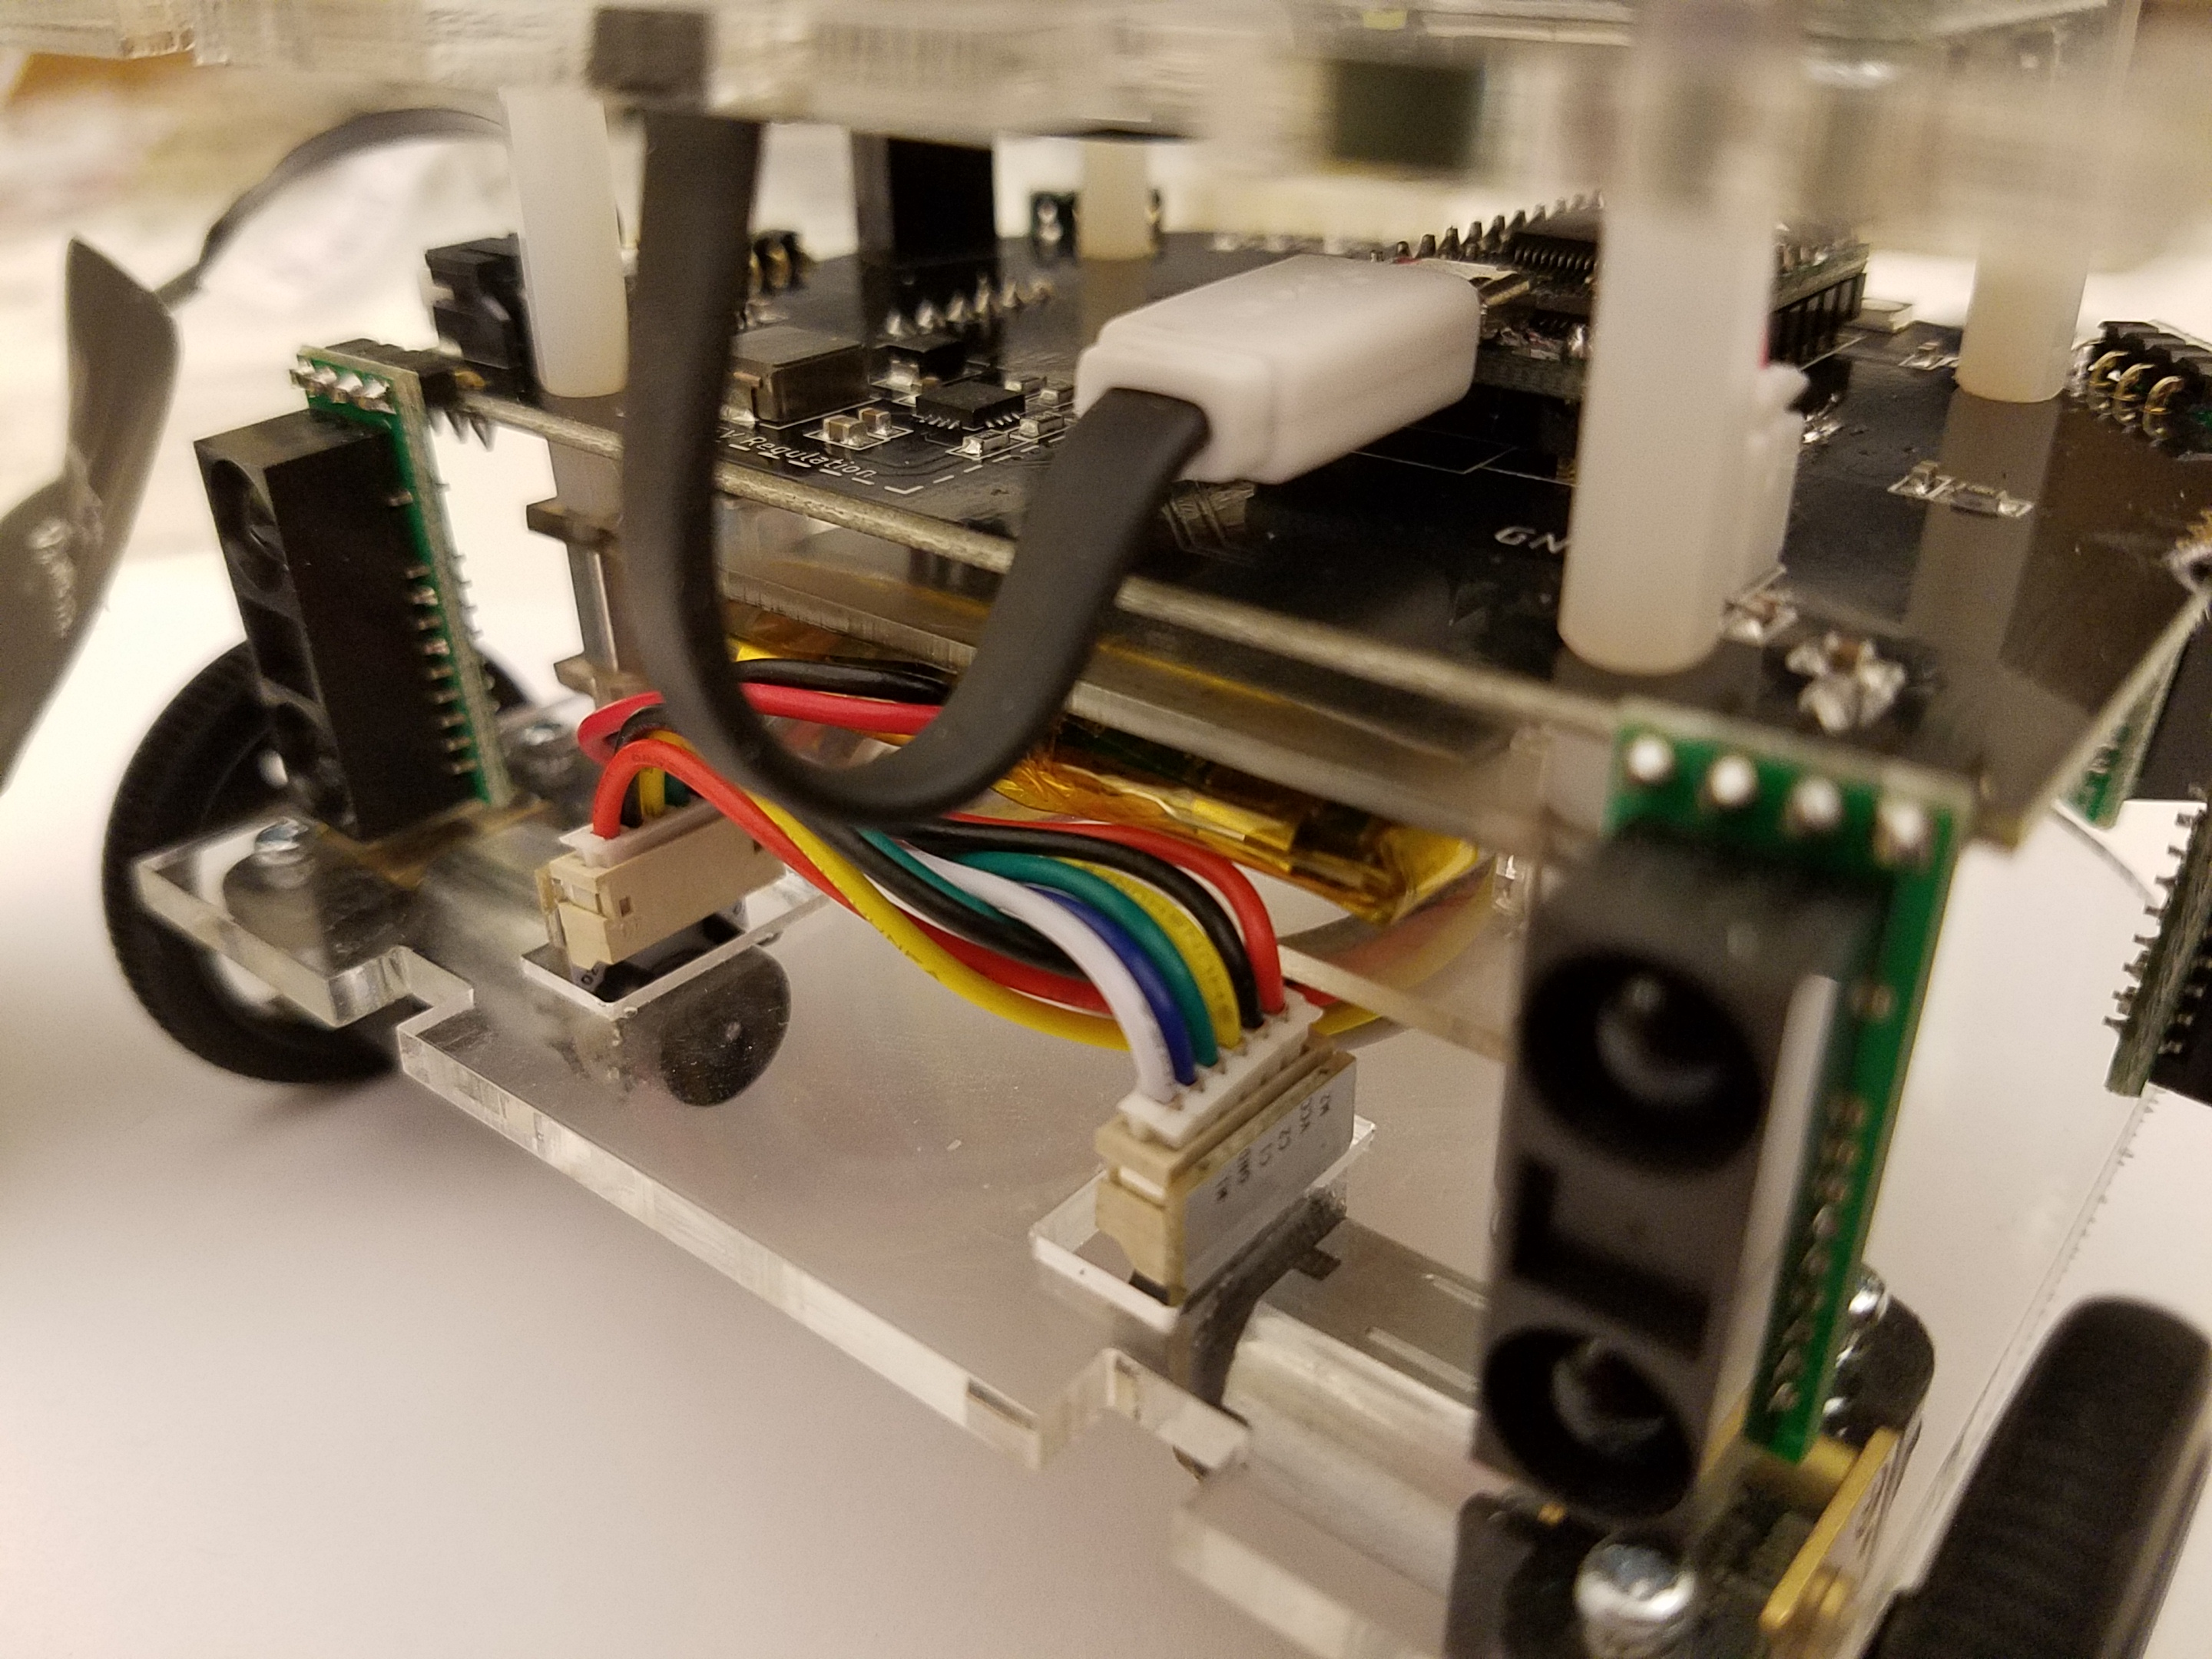
\includegraphics[width=0.45\columnwidth, keepaspectratio]{./figs/20190110_133153.jpg}}
\hfill
\subfloat[\label{fig:qiCharger} The Digiyes Qi charging reciever plugged in properly.]{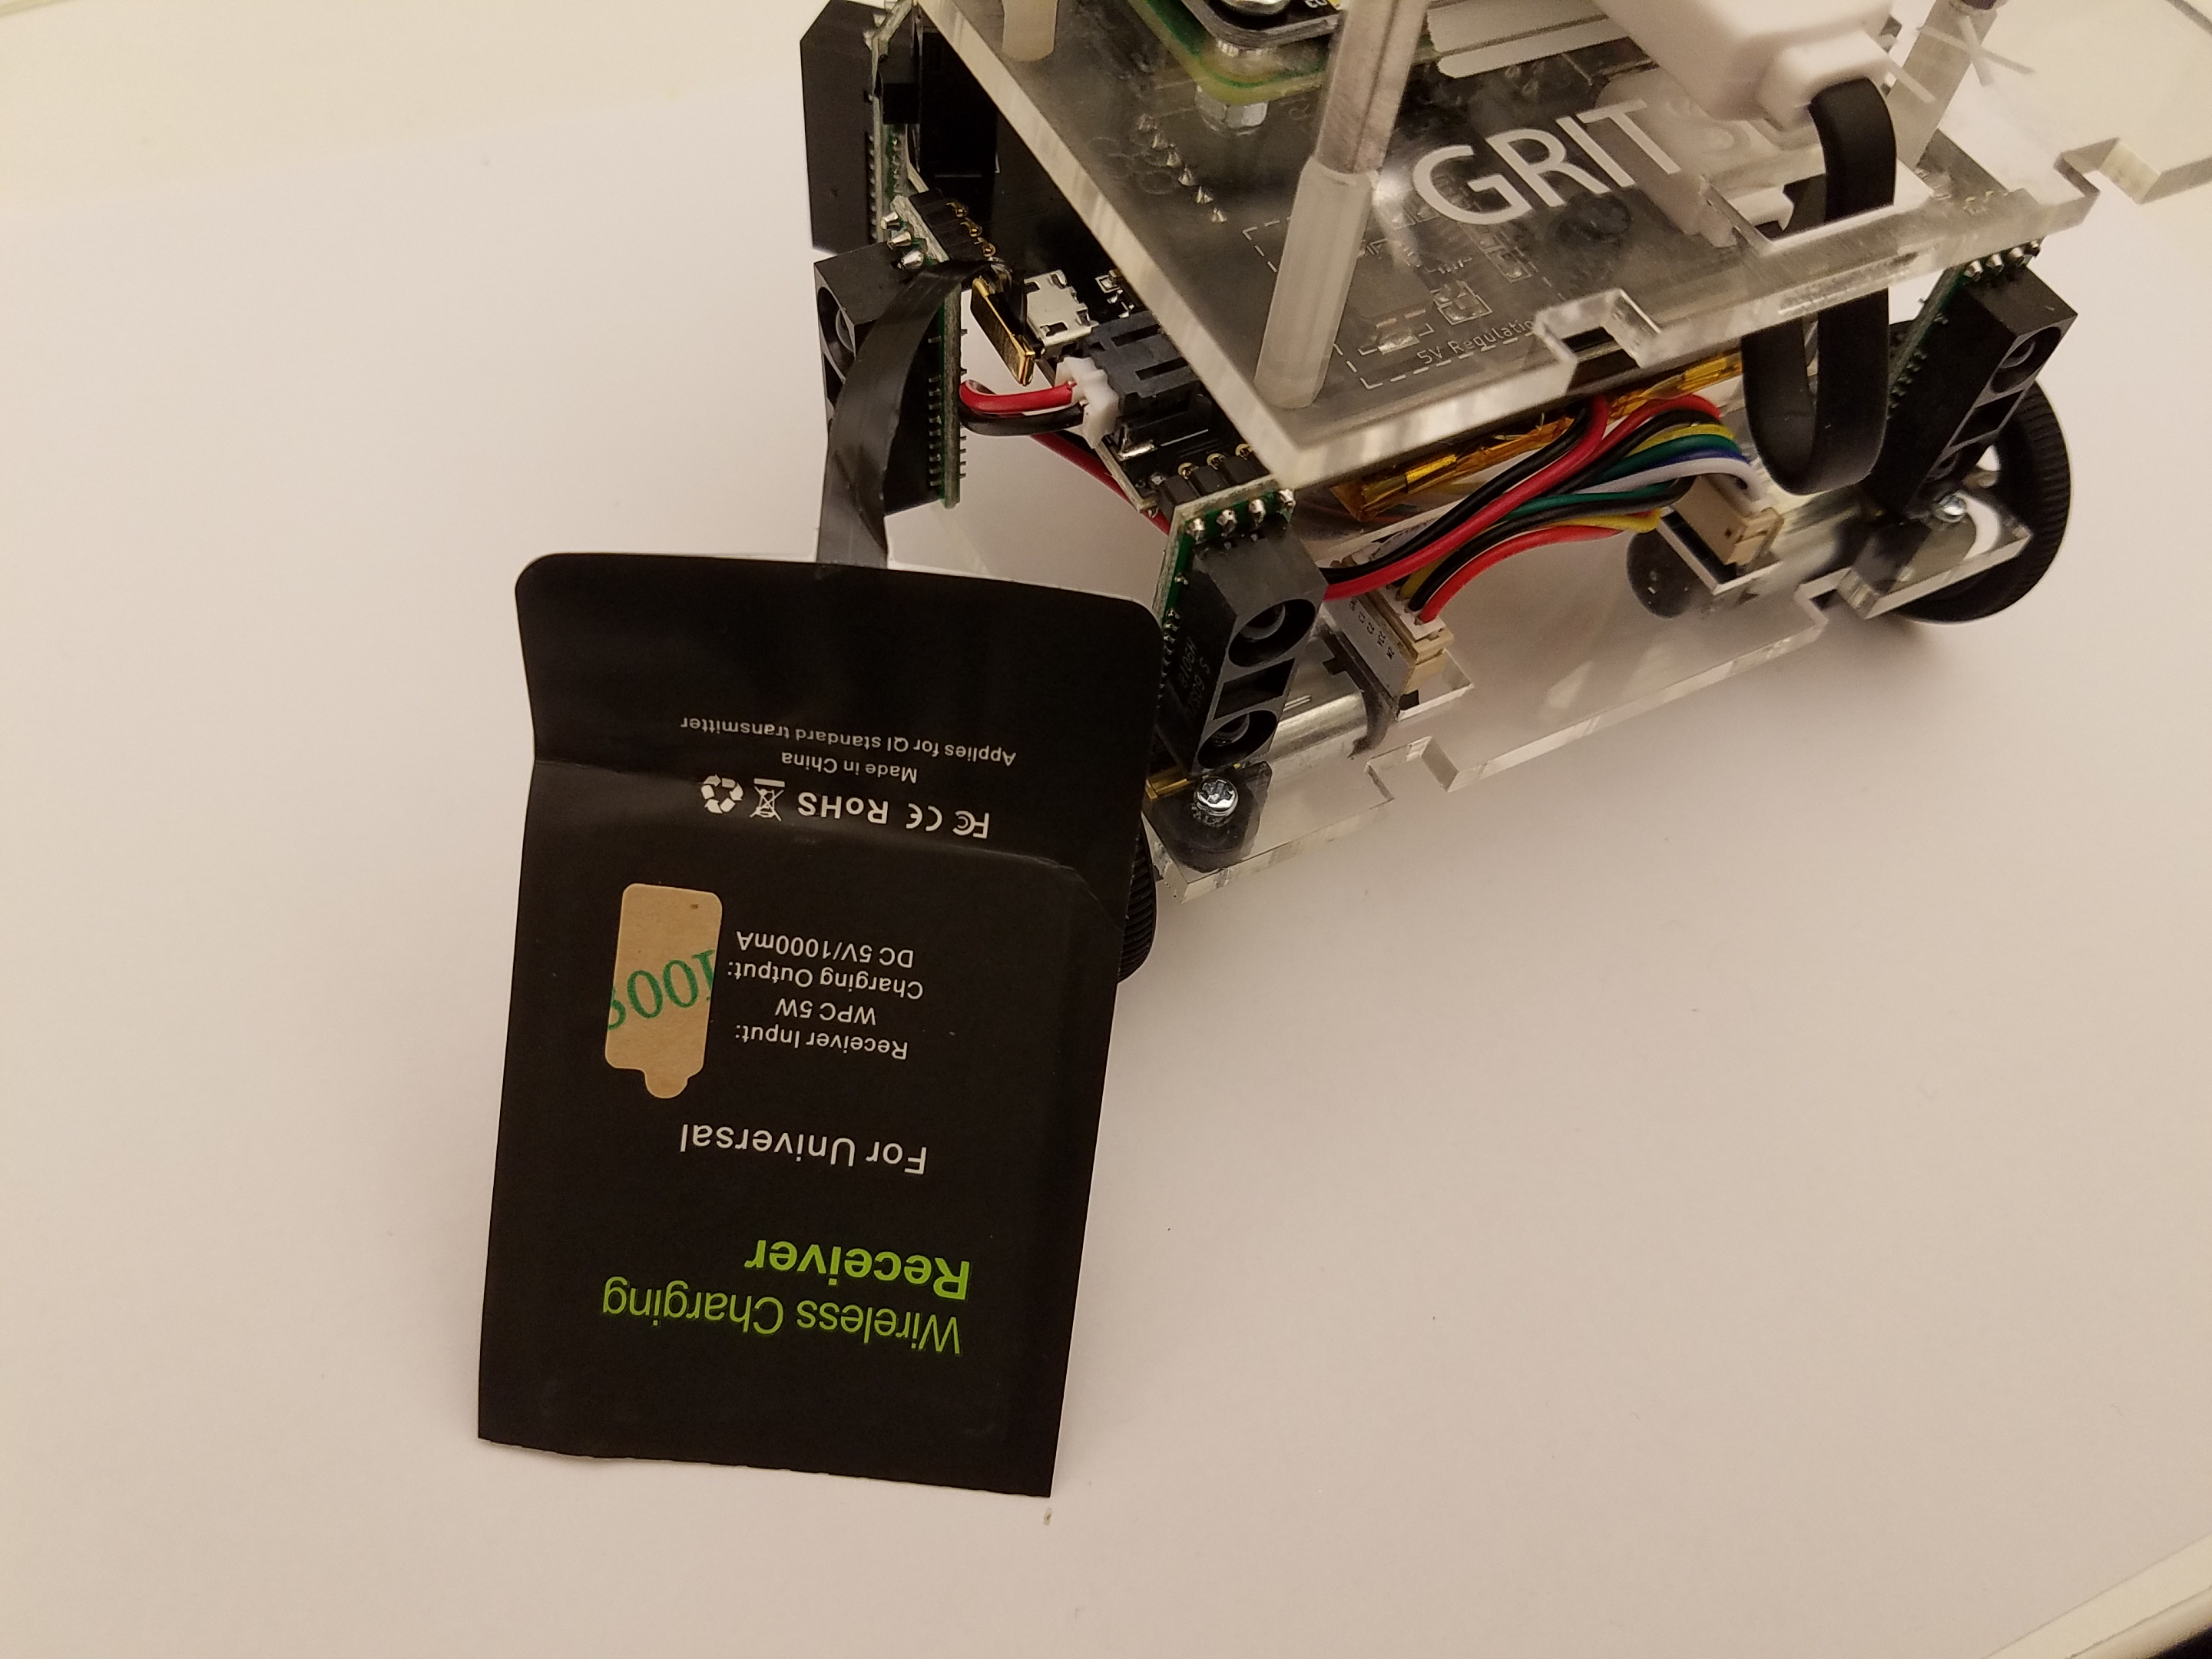
\includegraphics[width=0.45\columnwidth, keepaspectratio]{./figs/20190110_133139.jpg}}\\
\caption{The GRITSBot X with electronics properly attached.}
\label{fig:attachedElectronics}
\end{figure}
%End Electronics Plugged in Picture

\subsubsection{Attaching the Wireless Charger}
\label{sec:chargingPlate}

To finish the robot, the Qi wireless charger needs to be secured. Insert the acrylic back plate (the one without etching) of the charger into the slots in the top and bottom acylic plate of the chassis. It should slide in freely. Next, put the charging coil over this plate and fold the excess between the IR sensor and charging plate. It is best to route the connecting cable over the top of the PCB. {\color{red}{Do not}}, cover the IR sensor with the excess of the charging pad. Finally snap the front plate into the same four slots of the bottom and top of the chassis. Make sure the etching is facing out so the Robotarium logo is not reflected! If done correctly, the back of the robot should look like \cref{fig:finishedBack}.

%Final Back Picture
\begin{figure}[h!]
\centering
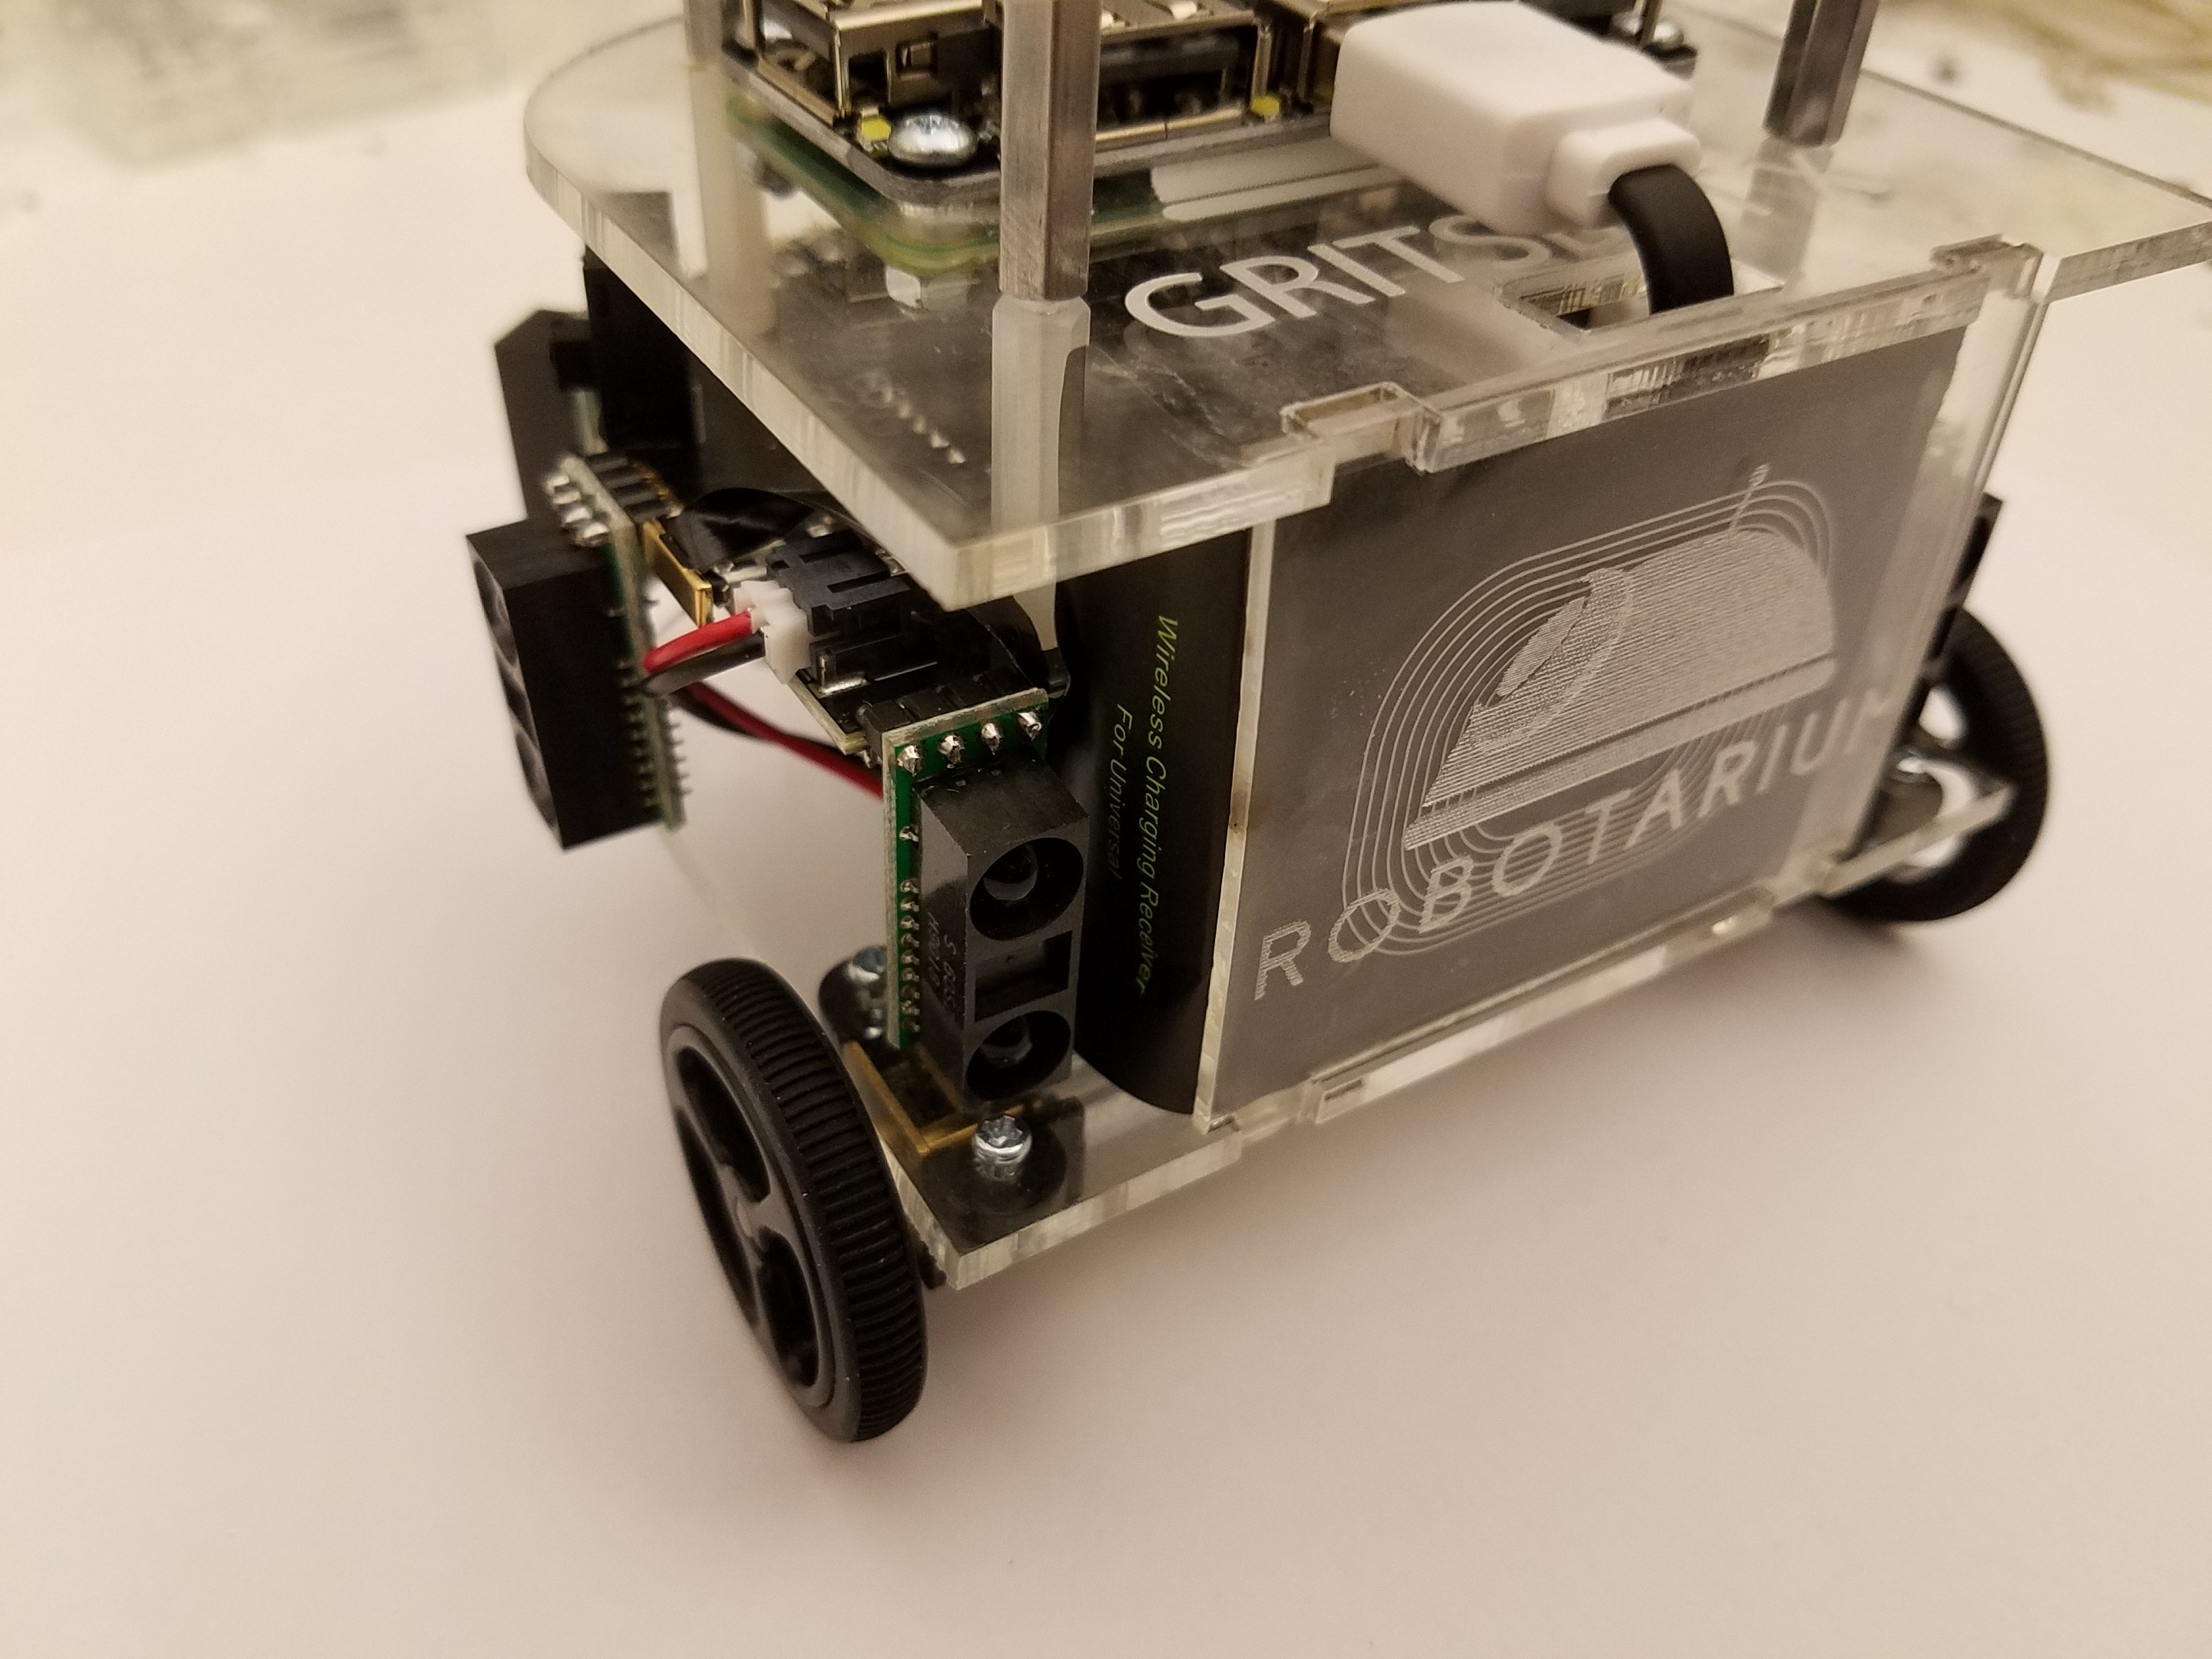
\includegraphics[width=0.65\columnwidth, keepaspectratio]{./figs/20190110_133256.jpg}
\caption{The charging plate of the GRITSBot X properly attached.}
\label{fig:finishedBack}
\end{figure}
%End Back  Picture


\subsubsection{CELEBRATE!}
\label{sec:CELEBRATE}

Congratulations! The GRITSBot X is completely assembled. You may move onto the next guide to get the software up and running and then begin programming your robot to do super cool tasks!